\documentclass[useAMS,usenatbib]{mn2e}                                  
%
%\def\del#1{{\bf  [deleted text] }} \def\new#1{{\bf #1}} \def\remark#1{{\bf  [remark: #1]}}
%\def\del#1{} \def\new#1{#1} \def\remark#1{}

\def\del#1{{}}
%\def\del#1{{\bf (DELETED TEXT)}}
\def\C#1{{\bf #1}}
%\def\C#1{#1}

%\newcommand{\rmn}{\mathrm}
\newcommand{\CR}{\mathrm{CR}}
\newcommand{\expval}[1]{\left\langle #1 \right\rangle}
\newcommand{\RA}[3]{#1$^{\mathrm{h}}$#2$^{\mathrm{m}}$#3$^{\mathrm{s}}$}
\newcommand{\Dec}[3]{#1$^{\circ}$#2\arcmin#3\arcsec}
\newcommand{\dps}{\displaystyle}
\newcommand{\eps}{\varepsilon}
\newcommand{\dd}{\mathrm{d}}
\newcommand{\vel}{\upsilon}
%
\usepackage{graphicx}
\usepackage{natbib}
%
\usepackage{txfonts}

%\voffset0.5in

%MNRAS
\title[On the Physics of Radio Halos in Galaxy Clusters]{On the Physics of Radio Halos in Galaxy Clusters: Scaling Relations and Luminosity Functions}
\author[F. Zandanel, C. Pfrommer and F. Prada]{
Fabio Zandanel$^{1 *}$, Christoph Pfrommer$^{2 \dagger}$ and Francisco Prada$^{3,4,1 \S}$\\
$^{1}$Instituto de Astrof\'{\i}sica de Andaluc\'{\i}a (CSIC), Glorieta de la Astronom\'{\i}a, E-18080 Granada, Spain\\
$^{2}$Heidelberg Institute for Theoretical Studies, Schloss-Wolfsbrunnenweg 35, D-69118 Heidelberg, Germany\\
$^{3}$Campus of International Excellence UAM+CSIC, Cantoblanco, E-28049 Madrid, Spain\\
$^{4}$Instituto de F\'{\i}sica Te\'orica, (UAM/CSIC), Universidad Aut\'onoma de Madrid, Cantoblanco, E-28049 Madrid, Spain}
\begin{document}

\date{Accepted XXX. Received XXX; in original from XXX}

\pagerange{\pageref{firstpage}--\pageref{lastpage}} \pubyear{2012}

\maketitle

\label{firstpage}

%%%%%%%%%%%%%%%%%%%%%%%%%%%%%%%%%%%%%%%
\begin{abstract}
  The underlying physics of giant radio halos and mini halos in galaxy clusters
  is still an open question, which becomes more pressing with the growing number
  of detections. We find that models where radio-emitting electrons are
  generated in hadronic cosmic ray (CR) proton interactions with protons of the
  intra-cluster medium provide nice matches to radio mini halos (Perseus,
  Ophiuchus). In contrast, the hadronic model either fails to explain the
  extended emission of giant radio halos (Coma at low frequencies) or would
  require a flat CR profile (A2163). Flat CR profiles can only be realized
  through CR streaming transport in {\em relaxed} clusters---in conflict with
  the observation that radio halos are hosted by merging {\em turbulent}
  clusters. This motivates us to propose a new hybrid model, where (i) mini
  halos are primarily of hadronic origin, (ii) giant halos experience a
  transition from central hadronic emission to peripheral leptonic emission due
  to Fermi I or II reacceleration of fossil or hadronically produced electrons,
  and (iii) steep spectrum radio sources are mainly of leptonic origin. We build
  a mock galaxy cluster catalog from the large MultiDark $N$-body $\Lambda$CDM
  simulation by adopting a phenomenological gas density model for each cluster
  based on X-ray measurements that matches Sunyaev-Zel'dovich and X-ray scaling
  relations and luminosity function. Because of the different scalings of the
  X-ray luminosity, $L_{\rmn{X}}$, and the Sunyaev-Zel'dovich flux, $Y$, with
  gas density and CR streaming transport, our model can simultaneously reproduce
  the observed bimodality of radio-loud and radio-quiet clusters at the same
  $L_{\rmn{X}}$ as well as the unimodal distribution of radio-halo luminosity
  versus $Y$; thereby suggesting a physical solution to this apparent
  contradiction. For a plausible fraction of 10\% radio-loud clusters, our model
  matches the NVSS radio-halo luminosity function. Constructing an analytical
  radio-halo luminosity function, we demonstrate the unique prospects for
  low-frequency radio surveys (such as the LOFAR Tier 1 survey) to detect
  $\sim3500$ radio halos back to redshift two and to probe the underlying
  physics of radio halos.  We will make our cosmologically complete
  multi-frequency mock catalogs for the (non-)thermal cluster emission at
  different redshifts publicly and freely available on-line through the
  MultiDark database.
\end{abstract}

\begin{keywords}
  Galaxies: clusters: intracluster medium - Radio continuum: galaxies - Gamma
  rays: galaxies: clusters - Astroparticle physics
\end{keywords}



%%%%%%%%%%%%%%%%%%%%%%%%%%%%%%%%%%%%%%%%%%%%%%%%%%%%%%%%%%%%%%%%%%%
%%%%%%%%%%%%%%%%%%%%%%%%%%%%%%%%%%%%%%%%%%%%%%%%%%%%%%%%%%%%%%%%%%%
\section{Introduction}
\label{sec:1}

\begingroup
\let\thefootnote\relax\footnotetext{* fabio@iaa.es}
\let\thefootnote\relax\footnotetext{$\dagger$ christoph.pfrommer@h-its.org}
\let\thefootnote\relax\footnotetext{$\S$ fprada@iaa.es}
\endgroup

The presence of large-scale diffuse radio synchrotron emission in clusters of
galaxies proves the existence of relativistic electrons and magnetic fields
permeating the intra-cluster medium (ICM) (see,
e.g, \citealp{2004NewAR..48.1137F}).  Diffuse cluster radio emission can be
separated in two classes: radio halos and radio relics (see,
e.g., \citealp{2004rcfg.procE..25K,2008SSRv..134...93F}).  Radio
\mbox{(mini-)}halos (RHs) are centered on clusters and characterized by a
regular and unpolarized morphology, resembling the morphology of the thermal
X-ray emission. On the contrary, radio relics typically lie at the cluster
outskirts, have an irregular morphology, and often show a high degree of
polarization. While relics seem to directly trace structure formation shocks
(e.g., \citealp{2011A&A...533A..35V}), the explanation for the RH phenomenon
is challenging and still an open question.
                                   
Two principal models have been proposed to explain RHs.  In the ``hadronic
model'' the radio emitting electrons are produced in hadronic cosmic ray (CR)
proton interactions with protons of the ambient thermal ICM, requiring only a
very modest fraction of (at most) a few percent of CR-to-thermal pressure
(\citealp{1980ApJ...239L..93D,1982AJ.....87.1266V, 1999APh....12..169B,
  2000A&A...362..151D, 2001ApJ...562..233M,2001ApJ...559...59M,
  2003MNRAS.342.1009M,2003A&A...407L..73P, 2004A&A...413...17P,
  2004MNRAS.352...76P, 2007IJMPA..22..681B, 2008MNRAS.385.1211P,
  2008MNRAS.385.1242P, 2009JCAP...09..024K, 2010MNRAS.401...47D,
  2010arXiv1003.0336D, 2010arXiv1003.1133K, 2010arXiv1011.0729K,
  2011A&A...527A..99E}).  CR protons and heavier nuclei, like electrons, can be
accelerated and injected into the ICM by structure formation shocks, active
galactic nuclei (AGN) and galactic winds.  Due to their higher masses with
respect to electrons, CR protons are accelerated more efficiently to
relativistic energies and are expected to show a ratio of the spectral energy
flux of CR protons to electrons above 1 GeV of about 100, similarly to what is
observed in our Galaxy \citep{2002cra..book.....S}. Additionally, CR protons
have a radiative cooling time larger than that of the electrons by the square of
the mass ratio and therefore can accumulate in clusters for cosmological times
\citep{1996SSRv...75..279V}. Indeed, CR electrons suffer more severe energy
losses via synchrotron and inverse Compton emission at particle energies $E
\gtrsim 100$~MeV, and Coulomb losses below that energy range.

In the ``re-acceleration model'', RHs are thought to be the result of
re-acceleration of electrons through interactions with plasma waves during
powerful states of ICM turbulence, as a consequence of a cluster merger
(\citealp{1987A&A...182...21S, 1993ApJ...406..399G, 2002A&A...386..456G,
  2004MNRAS.350.1174B, 2005MNRAS.363.1173B, 2007MNRAS.378..245B,
  2010arXiv1008.0184B, 2009A&A...507..661B, 2012arXiv1211.3337D}). This,
however, requires a sufficiently long-lived CR electron population at energies
around 100~MeV which has to be continuously maintained by re-acceleration at a
rate faster than the cooling processes.  We refer the reader to
\citet{2011A&A...527A..99E} for a discussion on the strengths and weaknesses of
these two models.

RHs can be divided in two classes. Giant radio halos are typically associated
with merging clusters and have large extensions, e.g., the Coma radio halo has
an extension of about 2~Mpc. Radio mini-halos are associated with relaxed
clusters that harbor a cool core and typically extend over a few hundred
kilo-parsecs, e.g., the Perseus radio mini-halo has an extension of about
0.2~Mpc.  The observed morphological similarities with the thermal X-ray
emission suggests that RHs may be of hadronic origin. In fact, cool-core
clusters (CCCs) are characterized by high thermal X-ray emissivities and ICM
densities that are more peaked in comparison to (merging) non cool-core clusters
(NCCCs) (e.g., \citealp{2008A&A...487..431C}). This distinct difference in the
ICM density structure of CCCs and NCCCs is reflected in the morphology of the
two observed classes of RHs.

The RH luminosity seems to be correlated to the thermal X-ray luminosity (e.g.,
\citealp{2009A&A...507..661B,2011A&A...527A..99E}).  However, a large fraction
of clusters does not exhibit significant diffuse synchrotron emission at current
sensitivity limits. Instead, stacking subsamples of luminous X-ray clusters
reveals a signal of extended diffuse radio emission that is about twice below
the radio upper limits on individual clusters \citep{2011ApJ...740L..28B};
suggesting that at least a subset of apparently ``radio-quiet'' clusters shows a
low-level diffuse emission. Galaxy clusters with the same thermal X-ray
luminosity show an apparent bimodality with respect to their radio
luminosity. Either they harbor a RH or they do not have any detectable diffuse
radio emission \citep{2009A&A...507..661B,2011A&A...527A..99E}. This suggests
the existence of a switch-on/switch-off mechanism that is able to change the
radio luminosity by more than one order of magnitude.  While such a mechanism
could be easily realized in the framework of the re-acceleration model
\citep{2009A&A...507..661B}, the \emph{classical} hadronic model predicts the
presence of RHs in all clusters. The failure to reproduce the observed cluster
radio-to-X-ray bimodality was one of the main criticisms against the hadronic
model.  Additionally, the \emph{classical} hadronic model cannot reproduce some
spectral features observed in clusters, such as the total spectral (convex)
curvature claimed in the Coma radio halo or the spectral steepening observed at
the boundary of some RHs. However, the recent report of spectral flattening with
frequency of the radio halo in A2256 \citep{2012A&A...543A..43V} could easily be
accommodated in the hadronic model, which naturally produces such a concave
spectrum \citep{2010MNRAS.409..449P}. This rises the interesting question
whether such a variability among different sources that are generally classified
as `radio halos' signals the presence of richer underlying physics---a question
that we will address in this paper.

In a recent work, \cite{2011A&A...527A..99E} assess these problems of the
\emph{classical} hadronic model by analyzing CR transport processes within a
cluster. While CR advection with turbulently driven flows results in centrally
enhanced CR profiles, the propagation in form of CR streaming and diffusion
produces a flattening of CR profiles. Hence, different CR transport phenomena
may also account for the observed bimodality of the radio luminosity in the
hadronic model and may also explain the spectral features observed in some
clusters \citep{2011A&A...527A..99E}. Note that these CR transport phenomena
were not considered in earlier analytical works (e.g.,
\citealp{2004A&A...413...17P}) as well as in previous hydrodynamic simulations
(e.g., \citealp{2001ApJ...562..233M, 2008MNRAS.385.1211P,
  2010MNRAS.409..449P}).

More recently, \cite{2012MNRAS.421L.112B} presented the first scaling relations
between RH luminosity and Sunyaev-Zel'dovich (SZ) flux measurements, using the
\emph{Planck} cluster catalogue. While the correlation agrees with previous
scaling measurements based on X-ray data, there is no indication for a bimodal
cluster population dividing clusters into radio-loud and radio-quiet objects at
fixed SZ flux. While the SZ flux correlates tightly with cluster mass, the X-ray
luminosity, $L_\rmn{X}$, exhibits a larger scatter. The CCCs predominantly
populate the high-$L_\rmn{X}$ tail (at any cluster temperature) and make up
approximately half of the radio-quiet objects \citep{2011A&A...527A..99E}. This
suggests that the switch-on/switch-off mechanism may not operate at fixed
$L_\rmn{X}$ but also causes an evolution of that quantity. As the cluster
relaxes after a merger, it cools and forms a denser core. Simultaneously,
$L_\rmn{X}$ is expected to {\em increase} which may simultaneously {\em
  decrease} the radio luminosity owing to the decaying turbulence that is
responsible in maintaining the radio emission in either model (that accounts for
microscopic CR transport).
 
An observational test that is able to disentangle between the hadronic and
re-acceleration models is the gamma-ray emission resulting from neutral pion
decays, a secondary product of the hadronic CR interaction with protons of the
ICM, which is not predicted by the re-acceleration model. Such observational
efforts have been undertaken in the last few years (for space-based cluster
observations in the GeV-band, see \citealt{2003ApJ...588..155R,
  2010JCAP...05..025A,2010ApJ...717L..71A,2012AAS...21920701Z,2012arXiv1207.6749H}; for ground-based
observations in the energy band $\gtrsim100$~GeV, see
\citealt{2006ApJ...644..148P, 2008AIPC.1085..569P,
  2009arXiv0907.0727T,2009A&A...495...27A, 2009arXiv0907.3001D,
  2009arXiv0907.5000G, cangaroo_clusters, 2009ApJ...706L.275A,
  2010ApJ...710..634A, 2011arXiv1111.5544M,2012...VERITAS,2012A&A...545A.103H})
without being able to detect cluster gamma-ray emission.  Gamma-ray limits
enable us to put significant constraints on the relative CR pressure
contributions. The long observational campaign of the Perseus galaxy cluster
performed by the Major Atmospheric Gamma-ray Cherenkov (MAGIC) telescopes
constrains the cluster average CR-to-thermal pressure to be less than a few
percent \citep{2010ApJ...710..634A,2011arXiv1111.5544M}. Comparing the
corresponding upper limits to predictions of simulations by
\cite{2010MNRAS.409..449P} constrains the maximum CR acceleration efficiency at
structure formation shocks to be $<50\%$.  Alternatively, this may indeed
suggest the presence of non-negligible CR transport processes into the outer
cluster regions as suggested by \cite{2011A&A...527A..99E}.  Constraints at the
same level are confirmed by the \emph{Fermi}-Large Area Telescope (LAT) data on
the Coma cluster \citep{2011arXiv1105.3240P,2012AAS...21920701Z,
  2012...VERITAS,2012arXiv1207.6749H}. To summarize, gamma-ray observations are not yet sensitive
enough to severely challenge hadronic models of RHs.

An important step towards understanding the generating mechanism of RHs could
come from detailed RH population analyses. To date, we know of 53 clusters that
harbor RHs (\citealp{2012A&ARv..20...54F}, for an almost up-to-date list). Only
two X-ray flux-limited studies have been conducted that assess the important
question of the RH frequency in clusters \citep{1999NewA....4..141G,
  VenturiGMRT_2}. Since the number of RHs in such X-ray flux-limited samples is
small with typically a few RHs, the conclusions on the underlying physical
mechanisms of RHs are not very robust. Fortunately, this is expected to change
thanks to the next-generation of low-frequency radio observatories such as the
Low Frequency Array (LOFAR).\footnote{www.lofar.org} In fact, a deep cluster
survey is part of the LOFAR science key projects and expected to provide a large
number of radio-emitting galaxy clusters up to redshift $z\approx1$ (e.g.,
\citealp{2010A&A...509A..68C,2012JApA..tmp...34R}). This will hopefully permit
to clearly determine the RH phenomenology with respect to cluster properties
such as the fractions of radio-loud/quiet, non cool-core/cool-core, and
non-merging/merging clusters, and to explore the role of different parameters
like the magnetic field, the CR acceleration efficiency, and CR transport
properties.

The outline is as follows. In Section~\ref{sec:2}, we explain the methodology of
assigning gas density profiles to dark matter (DM) halos and demonstrate that
the model reproduces the observed SZ and X-ray scaling relations and luminosity
function.  We then construct a model for the CR proton distribution in clusters
that merges results of hydrodynamic cluster simulations and an analytical model
for microscopic CR transport processes. In Section~\ref{sec:3}, we model
observed surface brightness profiles of individual RHs within the hadronic
scenario, explore the allowable parameter space for CRs and magnetic fields, and
discuss possible biases of our modeling approach.  Motivated by immanent
challenges to explain the extend of giant radio halos at low frequencies within
the hadronic model, we propose a new hybrid leptonic/hadronic scenario meant to
unify the apparently distinct classes of giant radio halos, mini halos, and
steep spectrum radio sources in Section~\ref{sec:discussion_hadronic}.  In
Section~\ref{sec:4}, we compare the modeled radio-to-X-ray and radio-to-SZ
scaling relations to current observations and show how they vary for different
choices of our CR and magnetic parametrizations. In Section~\ref{sec:5}, we show
the radio luminosity functions, compare them to current observational
constraints and provide predictions for the LOFAR cluster survey. Finally, in
Section~\ref{sec:6}, we present our conclusions. In this work, the cluster mass
$M_{\Delta}$ and radius $R_{\Delta}$ are defined with respect to a density that
is $\Delta=200$ or $\Delta=500$ times the \emph{critical} density of the
Universe. We adopt density parameters of $\Omega_{\rmn{m}}=0.3$,
$\Omega_{\Lambda}=0.7$ and today's Hubble constant of $H_0 = 100 \times
h_{70}$~km~s$^{-1}$~Mpc$^{-1}$ where $h_{70} = 0.7$.


%%%%%%%%%%%%%%%%%%%%%%%%%%%%%%%%%%%%%%%%%%%%%%%%%%%%%%%%%%%%%%%%%%%
%%%%%%%%%%%%%%%%%%%%%%%%%%%%%%%%%%%%%%%%%%%%%%%%%%%%%%%%%%%%%%%%%%%
\section{Methodology}
\label{sec:2}
The two basic ingredients of this work are an $N$-body, \emph{DM-only}
cosmological simulation that we use in constructing our complete cluster sample,
and the (non-)thermal emission model. Here, we use the MultiDark simulation that
will be described in Section~\ref{sec:2.1}, along with our final cluster
sample. As we will see, for any given cluster, the necessary ingredients for the
emission model are mass, temperature, and gas density distribution. We assign to
each cluster in that simulation a gas density profile that is phenomenologically
constructed from state-of-art X-ray observations, as will be shown in
Section~\ref{sec:2.2}. We will show that this approach can successfully
reproduce the known X-ray cluster characteristics, such as the X-ray luminosity
function (XLF), the luminosity-mass relation, $L_{\rmn{X}}- M$, and the
$Y_{\rmn{X}}-M$ relation, where $Y_{\rmn{X}}=M_\rmn{gas}k_{\rmn{B}}T$ with an
X-ray-derived gas mass $M_{\rmn{gas}}$ and temperature $T$
\citep{2006ApJ...650..128K}. Moreover, we compare our $Y_{\rmn{SZ}}-M$ relation
with SZ-derived measurements.  Only if our model matches available cluster data
on the gas properties, we can start to explore different parametrizations of CR
physics and its implications for the radio and gamma-ray emission, as will be
explained in Section~\ref{sec:2.3}.

%%%%%%%%%%%%%%%%%%%%%%
\subsection{MultiDark simulation and final cluster sample}
\label{sec:2.1}
The MultiDark simulation used in this work is described in detail in \cite{2011arXiv1104.5130P}.  
It is an $N$-body cosmological simulation done with
the Adaptive-Refinement-Tree (ART) code \citep{1997ApJS..111...73K} of
$2048^3$ particles within a ($1000$~Mpc~$h^{-1}$)$^3$ cube. The latest WMAP5 and
WMAP7 cosmological parameters were used. This simulation is particularly well
suited for our purpose because of its large number of clusters.
 
We use the MultiDark halo catalog from its on-line database,\footnote{www.multidark.org.} 
constructed with the Bound Density Maxima algorithm \citep{1997astro.ph.12217K}.  
We will mainly use $M_{500}$ and $R_{500}$ for comparison with existing observational works.  
We use the technique described in \cite{2003ApJ...584..702H} to convert $M_{200}$ and
$R_{200}$ provided by the MultiDark halo catalog to $M_{500}$ and $R_{500}$.  In
creating our cluster sample we only select distinct halos, i.e., those halos that
are not sub-halos of any other halo, which by definition are not galaxy clusters.

Additionally, we assume that the main emission mechanism in the ICM is thermal
bremsstrahlung, which is true only above a particle energy of approximately
$2.6$~keV \citep{1988xrec.book.....S}. Below this
energy, there could be other important contributions to the emission,
e.g., from atomic lines. Therefore, we impose a mass cut of
$M_{200}\geq1\times10^{14}$~$h^{-1}$~M$_{\odot}\approx1.4\times10^{14}$~$h_{70}^{-1}$~M$_{\odot}$
which ensures $k_{\rmn{B}}T \gtrsim 2.6$~keV, assuming the $M_{500} - T_{\rmn{ci}}$ relation
of \cite{2010MNRAS.406.1773M}.

The LOFAR radio observatory is expected to detect RHs up to redshift $z \approx
1$. Thus, we make use of different simulation snapshots up to $z=1$. In
Table~\ref{tab:z}, we show the total cluster number in our final cluster sample
at different redshifts.

\begin{table} 
\begin{center}
\caption{Number of halos in the final cluster sample}
\medskip
\begin{tabular}{cc}
\hline
\phantom{\Big|}
redshift $z$ & number of halos \\
\hline\\[-0.5em]
 0.0~~ &  13763\\
 0.1~~ &  12398\\
 0.2~~ &  10783\\ 
 0.4~~ &   ~~7789\\ 
 0.61  &  ~~5187\\ 
 0.78  &  ~~3372\\ 
 1.0~~ &  ~~1803\\[0.5em]
\hline
\end{tabular}
\label{tab:z}
\end{center}
\footnotesize{Note. We show the number of halos in our MultiDark snapshots at redshift $z$ for $M_{200}\geq1\times10^{14}$~$h^{-1}$~M$_{\odot}\approx1.4\times10^{14}$~$h_{70}^{-1}$~M$_{\odot}$. }
\end{table}


%%%%%%%%%%%%%%%%%%%%%%%%%%%%%%%%%%%%%%%%%%%%%%%%%%%%%%%%%%%%%%%%%%%
\subsection{Gas density modeling}
\label{sec:2.2}

We decided to use a \emph{phenomenological} approach and to construct the gas
density profiles directly from X-ray observations. A suitable X-ray sample that
provides the needed information is the \emph{Representative XMM-Newton Cluster
  Structure Survey} (REXCESS) sample \citep{2008A&A...487..431C,
  2009A&A...498..361P}. It is a sample of 31 galaxy clusters of different
dynamical states at redshifts $0.06<z<0.18$ with detailed information on the
de-projected electron density profiles \citep{2008A&A...487..431C}. In
Fig.~\ref{fig:gas_profiles}, we show the 31 electron density profiles of the
REXCESS sample color-coded by CCCs and NCCCs.

In order to obtain an electron density profile that we will attach to our
simulated clusters, we use a generalized Navarro-Frank-White (GNFW) profile,
\begin{equation}
n_{\rmn{e}}(x) = \frac{n_{0}}{x^{\beta}\left[1+x^{\alpha}\right]^{\frac{\delta-\beta}{\alpha}}},
\label{eq:gnfw}
\end{equation}
where $x=R/R_{\rmn{c}}$ and $R_{\rmn{c}}$ is the cluster core radius. To reduce
the dimensionality of our fit, we fix representative values of $R_{\rmn{c}} =
0.2\, R_{500}$, $\alpha = 1$ and $\delta = 2.5$. We fit the radial density
profiles of the REXCESS sample in log-log space, separating them in the two
categories of NCCCs and CCCs as shown in Fig.~\ref{fig:gas_profiles}.  We
obtain $n_{\rmn{0,NCCC}} = 1.02\times10^{-2}$~$h_{70}^{1/2}$~cm$^{-3}$,
$n_{\rmn{0,CCC}} = 8.32\times10^{-3}$~$h_{70}^{1/2}$~cm$^{-3}$,
$\beta_{\rmn{NCCC}} = -0.093$, and $\beta_{\rmn{CCC}} = 0.592$. The resulting
fits are shown in blue and red for the NCCC and CCC population, respectively.

The next step is to introduce a mass-scaling in order to apply our GNFW profiles
to all our clusters. We adopt the gas mass fraction-mass scaling,
$f_{\rmn{gas},500}-M_{500}$ of \cite{2009ApJ...693.1142S} (and adopt their equation~(8)). We can
express $f_{\rmn{gas},500}$ in the following way:
\begin{equation}
f_{\rmn{gas},500} = \frac{M_{\rmn{gas},500}}{M_{500}}  = \frac{\int_{0}^{R_{500}} \rho_{\rmn{gas}} \rmn{d}V}{M_{500}}
\label{eq:m500}
\end{equation}
with $\rho_{\rmn{gas}}(R) = \rho_{\rmn{gas}} = n_{\rmn{e}} m_{\rmn{p}} / ( X_{\rmn{H}}X_{\rmn{e}} )$ where
$m_{\rmn{p}}$ is the proton mass, $X_{\rmn{H}} = 0.76$ is the primordial hydrogen
mass fraction and $X_{\rmn{e}} = 1.157$ the ratio of electron-to-hydrogen number
densities in the fully ionized ICM \citep{1988xrec.book.....S}. For each cluster
$i$ of our sample, we then define a \emph{mass-scaled} gas profile as
$\rho_{\rmn{gas},i}=C_{i} \,\rho_{\rmn{gas}}$ with:
\begin{eqnarray}
%C_{i}  =  (0.0616\pm(0.0060g_{1}))  h_{73}^{-1.5}  \left(\frac{M_{500,i}}{10^{13} h_{73}^{-1} \rmn{M_{\odot}}}\right)^{0.135\pm(0.030g_{2})} \nonumber \\
C_{i}  & = &  (0.0656\pm(0.0064g_{1})) \, h_{70}^{-1.5}  \nonumber \\
 & \times & \left(\frac{M_{500,i}}{1.04 \times 10^{13} h_{70}^{-1} \rmn{M_{\odot}}}\right)^{0.135\pm(0.030g_{2})} \frac{M_{500,i}}{\int_{0}^{R_{500,i}} \rho_{\rmn{gas}} \rmn{d}V}
\label{eq:gas_scaling}
\end{eqnarray}
where $g_{1}$ and $g_{2}$ are random Gaussian number which we use in order to
simulate the natural scatter of the gas profiles.\footnote{The values
  $0.0064$ and $0.03$ quoted in equation~(\ref{eq:gas_scaling}) do not represent
  the proper scatter of the $f_{\rmn{gas},500}-M_{500}$ relation but reflect the
  parameter errors and we rescaled the numerical values to a Hubble constant of
  $h_{70}$ used in this work.}

\begin{figure} 
\centering
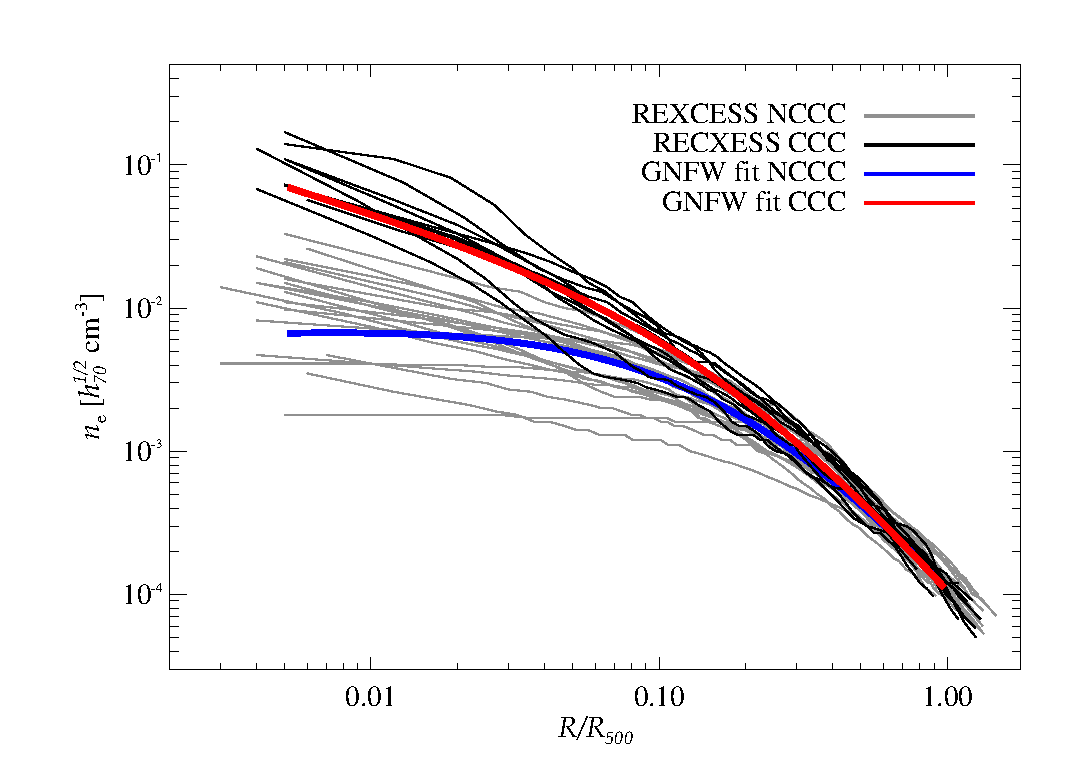
\includegraphics[width=0.5\textwidth]{figures/gas_profiles.eps}
\caption{Electron density profiles of the 31 clusters in the REXCESS sample. Grey and black lines represent NCCCs and CCCs, respectively. The blue and red lines represent our GNFW mean profile for the NCCCs and CCCs, respectively.}
\label{fig:gas_profiles}
\end{figure}

Hence, for each cluster in our sample we obtain a gas density profile
$\rho_{\rmn{gas},i}$ that obeys the observed $f_{gas,500}-M_{500}$ relation and
is uniquely determined by its DM mass $M_{500,i}$ and by the property of being a
NCCC or CCC. We assign the latter property to every halo depending on its
merging history. In particular, we make use of the offset parameter
$X_{\rmn{off}}$ computed for the MultiDark halo catalog. This is defined as the
distance from the halo center to the center of mass in units of the virial
radius. This parameter assesses the dynamical state of the cluster and whether
the halo experienced a recent merger or not. Current observations reveal a ratio
of NCCCs and CCCs of about $50\%$ (e.g., \citealp{2007A&A...466..805C,
  2009MNRAS.395..764S}). Since there is a correlation between merging clusters
and NCCCs, we use the median of the $X_{\rmn{off}}$ distribution to separate our
sample into CCCs and NCCCs (with NCCCs defined to be those halos with the larger
dynamical offsets). Clearly, this is an over-simplification, and future X-ray
surveys will have to determine this property also as a function of redshift.

We also account for redshift evolution of the gas profiles. While our NCCC and
CCC gas profiles as derived from the REXCESS cluster sample are merely used to
define a profile shape, the normalization of the gas profiles is set by the
observational $f_{\rmn{gas},500}-M_{500}$ relation \citep{2009ApJ...693.1142S}.
The 43 clusters used in \cite{2009ApJ...693.1142S} have redshifts $0.012 < z <
0.12$ with a \emph{median} of $z \approx 0.04$. Thus, our phenomenological gas
profile is representative of the cluster population at $z\approx0$. To extend this
profile to high-$z$, we include a \emph{self-similar} scaling of the gas density
as $\rho_{\rmn{gas}}(z) = E(z)^{2} \rho_{\rmn{gas}}(z=0)$, where $E(z)^{2} =
\Omega_{\rmn{m}} (1+z)^{3} + \Omega_{{\Lambda}}$.


\subsection{X-ray and SZ scaling relations}
\label{sec:X-SZ-scaling}

In order to check whether our phenomenologically derived gas profiles reproduce
the observations, we calculate the bolometric thermal bremsstrahlung
luminosity $L_{\rmn{bol}}$ as in \cite{1988xrec.book.....S}\footnote{We check
  our procedure by fitting each of the 31 REXCESS clusters with
  equation~(\ref{eq:gnfw}) and calculating $L_{\rmn{bol}}$ with the measured gas
  temperature of each cluster. As a result, we fall short of the observed
  luminosity by a mean (median) of about $21\%$ ($20\%$). This is reasonable
  considering that we do not permit the parameters $R_{\rmn{c}}$, $\alpha$ and
  $\delta$ to vary between different objects. Additionally, we neglect atomic
  line emission which may give a noticeable contribution, in particularly for
  low-mass clusters and in the cluster outskirts of larger systems.}  and
compare our sample result with the observed $L_{\rmn{bol}} - M_{500}$ relation
and XLF.\footnote{The mean (median) difference at $z=0$ between
  $L_{\rmn{bol}}$ within $R_{200}$ or within $R_{500}$ is $\approx 5\%$ ($\approx
  7\%$). While $L_{\rmn{bol}}$ refers to the quantity calculated within
  $R_{500}$, we note that the XLF for luminosities calculated within $R_{200}$
  will be barely changed.}

To assign a temperature to our model clusters (that is needed for calculating
$L_{\rmn{bol}}$ and $Y_{\rmn{X}}$), we adopt the $T-M_{500}$ relation by
\cite{2010MNRAS.406.1773M},
\begin{equation}
\log_{10} \left( \frac{k_{\rmn{B}}T_{\rmn{ci}}}{\rmn{keV}} \right) = 
A + B~\log_{10} \left( \frac{E(z) M_{500}}{10^{15} h_{70}^{-1} \rmn{M_{\odot}}} \right)
\label{eq:temp}
\end{equation}
where $A=0.91$, $B=0.46$, and $T_{\rmn{ci}}$ is the cluster temperature
\emph{not} centrally excised
(\citealp{2010MNRAS.406.1773M}). \cite{2010MNRAS.406.1773M} report a scatter of
$\sigma_{\rmn{yx}} = 0.06,$\footnote{Scatter is calculated as $\sigma_{\rmn{yx}}
  = \sqrt{ \left\{ \Sigma_{i=1}^{N} [Y_{i}-(A+B~X_{i})]^{2}\right\} / N-1}$
  where the sum extends over the data points $X_{i}, Y_{i}$, and $A$ and $B$ are
  the fit parameters.} which we apply to our sample using Gaussian deviates.

\begin{figure*} 
\centering
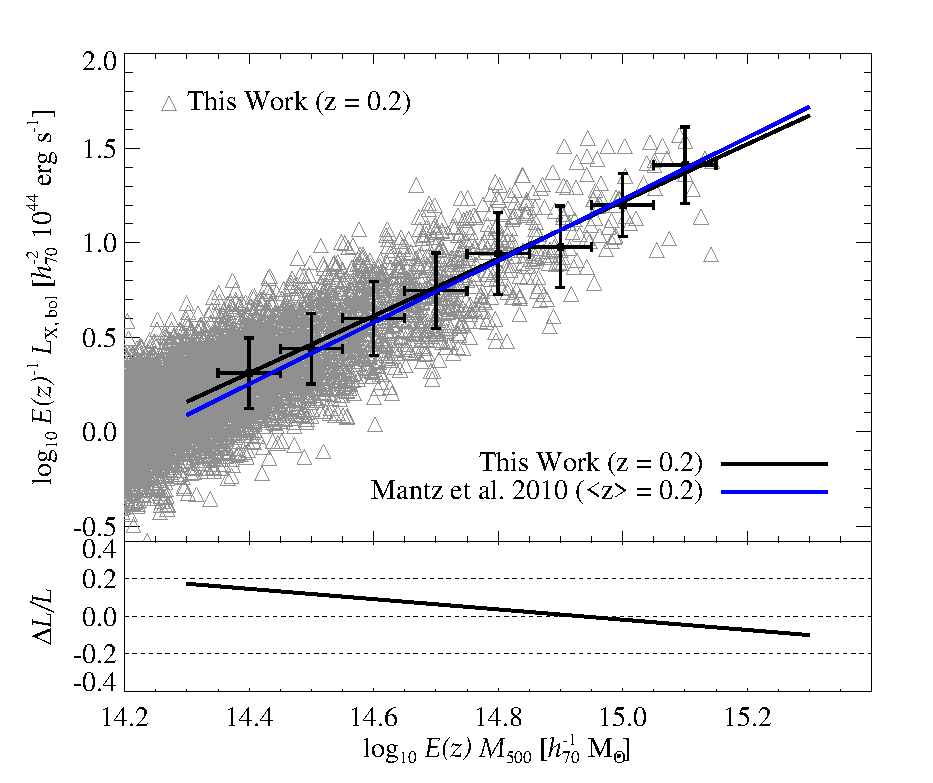
\includegraphics[width=0.33\textwidth]{figures/lx_m.eps}
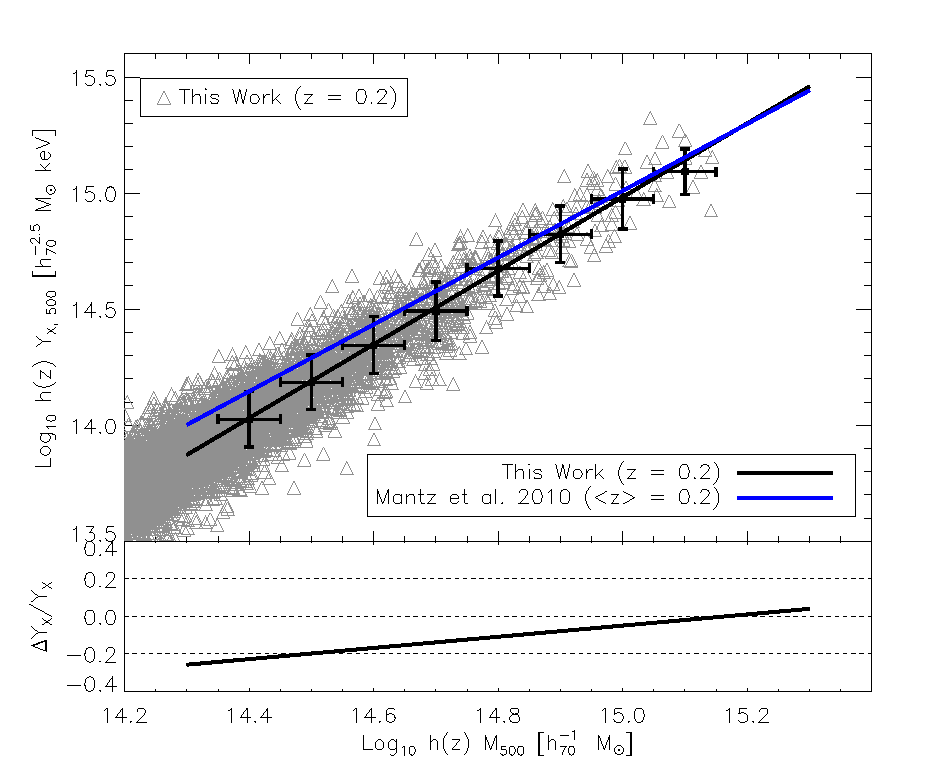
\includegraphics[width=0.33\textwidth]{figures/yx_m.eps}
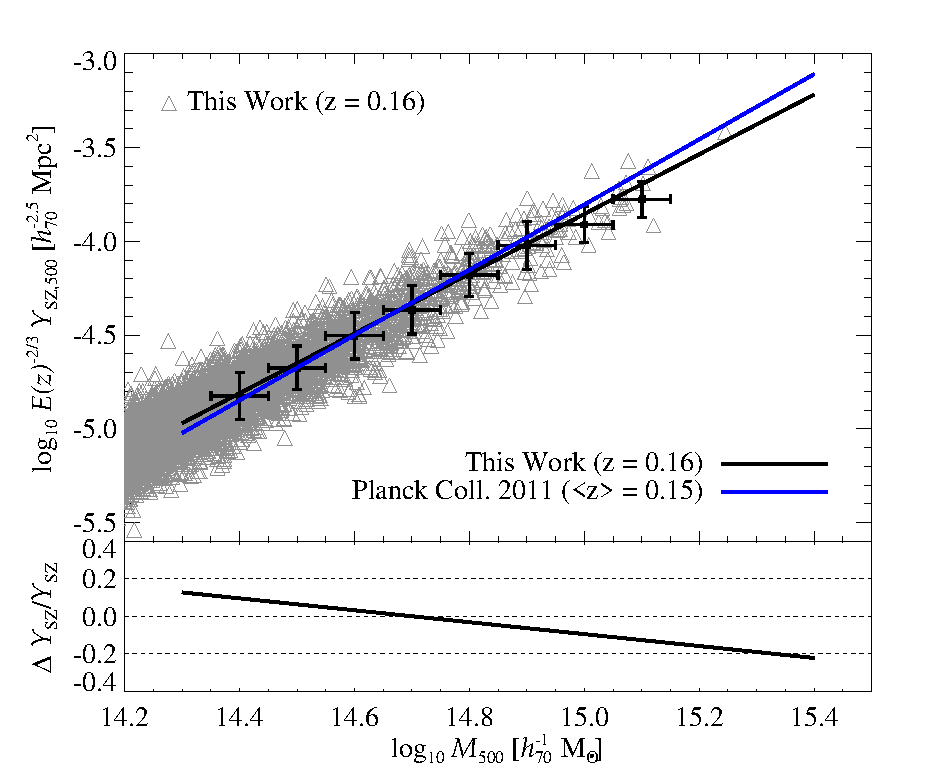
\includegraphics[width=0.33\textwidth]{figures/sz_m.eps}
\caption{X-ray and SZ scaling relations. Grey triangles show the MultiDark
  sample (limited to the mass range covered by observations), the black line is
  the corresponding scaling relation, and the blue line is the
  observational result. The black crosses represent the median values of the
  quantity in question for a given mass bin (indicated by horizontal error
  bars), and the vertical error bars represent the standard deviation within a
  bin.  \emph{Left.} We compare the bolometric X-ray luminosity-to-mass
  relation, $L_{\rmn{bol}}-M_{500}$, at $z=0.2$ to the observational sample by
  \protect\cite{2010MNRAS.406.1773M} with a median of $z \approx 0.2$. \emph{Center.}
  $Y_{\rmn{X}}-M_{500}$ scaling relation of our model in comparison to the
  observational sample by \protect\cite{2010MNRAS.406.1773M}. \emph{Right.}
  $Y_{\rmn{SZ}}-M_{500}$ scaling relation at $z=0.16$ in comparison
  to the observational sample by the \protect\cite{2011A&A...536A..11P} with a median
  redshift of about $0.15$. The bottom panels show the relative difference to
  the observational scaling relations.}
\label{fig:X_LM}
\end{figure*}

In the left panel of Fig.~\ref{fig:X_LM}, we show how our model
$L_{\rmn{bol}}-M_{500}$ relation compares with observations by
\cite{2010MNRAS.406.1773M} (\emph{all} data, see their Table~7). Their sample is
composed of 238 clusters at $0.02<z<0.46$ with a median of $z \approx 0.2$ and
self-consistently takes into account all selection effects, covariances,
systematic uncertainties and the cluster mass function
\citep{2010MNRAS.406.1759M}.  For this reason, we compare the
\cite{2010MNRAS.406.1773M} data to our model at $z=0.2$, and limit the
comparison to the mass range covered by the observations. Overall, there is
reassuring agreement between our phenomenological model and the data, which
probe our model most closely on scales around the cluster core radii (which is
where the contribution to $L_{\rmn{X}}$ per logarithmic interval in radius, $\dd
L_{\rmn{X}}/\dd\log r \propto r^3 n_{\rm{gas}}^2(r) \sqrt{k_{\rmn{B}}T}$,
approximately attains its maximum).  In Table~\ref{tab:LMfits}, we show our
model $L_{\rmn{bol}}-M_{500}$ scaling relation and its scatter for different
redshifts. We find that the scatter of our samples at all redshifts are Gaussian
distributed with a standard deviation of $\sigma_{yx} \approx 0.18$ that matches
the observational results of \cite{2010MNRAS.406.1773M}, which report a scatter
of $\sigma_{yx} = 0.185$.

In the middle panel of Fig.~\ref{fig:X_LM}, we compare the
$Y_{\rmn{X}}-M_{500}$ relation of our sample to observational data
\citep{2010MNRAS.406.1773M}. The model agrees nicely at the high-mass end, but
underpredicts the observed scaling at low masses by about $20\%$ (at the
1-$\sigma$ level). This is the same level of deviation from the data as in the
case of $L_{\rmn{X}}$, which is more significant due to the smaller scatter in
the $Y_{\rmn{X}}$ relation. The differential contribution to the thermal energy
per logarithmic interval in radius (and hence to the integrated Compton-$y$
parameter) is given by $\dd Y /\dd\log r \propto r^3 P_{\rmn{th}}(r)$, with the
thermal gas pressure $P_{\rmn{th}}=n_{\rmn{gas}}k_{\rmn{B}}T$. It peaks at
scales slightly smaller than $R_{500}$ with 1-$\sigma$ contributions extending
out to $3\,R_{500}$ \citep{2010ApJ...725...91B}. Hence, the observational
scaling constrains our model on those large scales, quite complementary to the
X-ray luminosity. The deviations at small masses either indicates different
assumptions about $f_{\rmn{gas}}$, the gas temperature, or different selection
effects of either observational sample that we use for model calibration and
comparison.  \cite{2010MNRAS.406.1773M} determine their masses by adopting a
constant value for $f_{\rmn{gas}}$, in contrast to our approach which adopts the
observed $f_{\rmn{gas},500}-M_{500}$ relation given by
\cite{2009ApJ...693.1142S}. Additionally, we adopt the
\cite{2010MNRAS.406.1773M} \emph{centrally included} temperature throughout all
our work, while \cite{2010MNRAS.406.1773M} use the \emph{centrally excised}
temperature to calculate $Y_{\rmn{X}}$. This assumption also impacts the scatter
of the $Y_{\rmn{X}}-M$ relation. In fact, using the \emph{centrally included}
temperature, we found a scatter of $\sigma_{yx} \approx 0.11$ (see
Table~\ref{tab:YXfits} where our $Y_{\rmn{X}}$ scaling relations are reported),
significantly higher than the value of $\sigma_{yx} = 0.052$ found by
\cite{2010MNRAS.406.1773M}.

In the right panel of Fig.~\ref{fig:X_LM}, we compare the
$Y_{\rmn{SZ}}-M_{500}$ relation in our model (calculated as in equation~(3) of
\citealp{2011arXiv1109.3709B}) with the observed scaling relation by the
\cite{2011A&A...536A..11P}. Their sample contains clusters up to $z \approx
0.45$ and has a median of $z \approx 0.15$; hence, we compare the data to our
relation at the MultiDark snapshot $z=0.16$ (that contains 11419 clusters above
our mass cut) which however is not used throughout the rest of the work. Our
model reproduces the data remarkably well, except for the high-mass end where
our simulations have a weaker constraining power due to the smaller box size in
comparison to the survey volume of {\em Planck}.  We find a scatter of
$\sigma_{yx} \approx 0.11$ which compares well with the \emph{Planck} result of
$\sigma_{yx} \approx 0.1$. In Table~\ref{tab:YSZfits}, we report our SZ scaling
relations for different redshifts.
 
\begin{table} 
\begin{center}
\caption{$L_{\rmn{bol}}-M_{500}$ scaling relations.}
\medskip
\begin{tabular}{cccc}
\hline
\phantom{\Big|}
redshift $z$ & $A$ & $B$ & $\sigma_{yx}$ \\
\hline \\[-0.5em]
 0      & $-21.41\pm0.11$ & $1.50\pm0.01$ & 0.179\\
 0.1   & $-21.30\pm0.12$ & $1.50\pm0.01$ & 0.179\\
 0.2   & $-21.50\pm0.13$ & $1.51\pm0.01$ & 0.178\\ 
 0.4   & $-21.13\pm0.17$ & $1.49\pm0.01$ & 0.178\\ 
 0.61 & $-21.59\pm0.22$ & $1.53\pm0.01$ & 0.177\\ 
 0.78 & $-20.73\pm0.29$ & $1.48\pm0.02$ & 0.177\\ 
 1      & $-20.45\pm0.42$ & $1.46\pm0.03$ & 0.177\\[0.5em]
\hline
\end{tabular}
\label{tab:LMfits}
\end{center}
\footnotesize{Note. Scaling relations are reported in the form of $\log_{10}~(L_{\rmn{bol}}~/~E(z)~h_{70}^{-2}~10^{44}~\rmn{erg~s}^{-1})=A+B~\log_{10}~(E(z)~M_{500}~/~h_{70}^{-1}~\rmn{M_{\odot}})$. The relation scatter $\sigma_{yx}$ is also shown.}
\end{table}
 
\begin{table} 
\begin{center}
\caption{$Y_{\rmn{X}, 500}-M_{500}$ scaling relations.}
\medskip
\begin{tabular}{cccc}
\hline
\phantom{\Big|}
redshift $z$ & $A$ & $B$ & $\sigma_{yx}$ \\
\hline\\[-0.5em]
 0      & $-9.18\pm0.07$ & $1.61\pm0.01$ & 0.109\\
 0.1   & $-8.85\pm0.07$ & $1.59\pm0.01$ & 0.109\\
 0.2   & $-8.82\pm0.08$ & $1.59\pm0.01$ & 0.109\\ 
 0.4   & $-8.79\pm0.10$ & $1.59\pm0.01$ & 0.108\\ 
 0.61 & $-8.65\pm0.14$ & $1.59\pm0.01$ & 0.109\\ 
 0.78 & $-8.36\pm0.18$ & $1.57\pm0.01$ & 0.109\\ 
 1      & $-8.28\pm0.26$ & $1.57\pm0.02$ & 0.109\\[0.5em]  
\hline
\end{tabular}
\label{tab:YXfits}
\end{center}
\footnotesize{Note. Scaling relations are reported in the form of $\log_{10}~(E(z)~Y_{\rmn{X},500}~/~h_{70}^{-2.5}~\rmn{M_{\odot}}~\rmn{keV})=A+B~\log_{10}~(E(z)~M_{500}~/~h_{70}^{-1}~\rmn{M_{\odot}})$. The relation scatter $\sigma_{yx}$ is also shown.}
\end{table}

\begin{table} 
\begin{center}
\caption{$Y_{\rmn{SZ}, 500}-M_{500}$ scaling relations.}
\medskip
\begin{tabular}{cccc}
\hline
\phantom{\Big|}
redshift $z$ & $A$ & $B$ & $\sigma_{yx}$ \\
\hline\\[-0.5em]
 0      & $-27.93\pm0.07$ & $1.60\pm0.01$ & 0.109\\
 0.1   & $-27.74\pm0.07$ & $1.59\pm0.01$ & 0.109\\
 0.16 & $-27.76\pm0.08$ & $1.59\pm0.01$ & 0.109\\
 0.2   & $-27.65\pm0.08$ & $1.59\pm0.01$ & 0.109\\ 
 0.4   & $-27.57\pm0.10$ & $1.59\pm0.01$ & 0.108\\ 
 0.61 & $-27.50\pm0.13$ & $1.59\pm0.01$ & 0.109\\ 
 0.78 & $-27.15\pm0.18$ & $1.58\pm0.01$ & 0.109\\ 
 1      & $-27.01\pm0.26$ & $1.58\pm0.02$ & 0.109\\[0.5em] 
\hline
\end{tabular}
\label{tab:YSZfits}
\end{center}
\footnotesize{Note. Scaling relations are reported in the form of $\log_{10}~(E(z)^{-2/3}~Y_{\rmn{SZ},500}~/~h_{70}^{-2.5}~\rmn{Mpc}^{2})=A+B~\log_{10}~(M_{500}~/~h_{70}^{-1}~\rmn{M_{\odot}})$. The relation scatter $\sigma_{yx}$ is also shown.}
\end{table}



\subsection{X-ray luminosity function}

Studies of the XLF got out of fashion during the last years due to the
difficulties of using the X-ray luminosity for cosmological purposes. The X-ray
emissivity scales with the square of the gas density, which makes it subject to
density variations and clumping. This implies large scatter that causes a large
Malmquist bias and underlines the necessity of careful mock surveys that need to
address all systematics.

Nevertheless, it provides a complementary check for our model. To this end, we
use the \emph{ROSAT} brightest cluster sample (BCS) XLF
\citep{1997ApJ...479L.101E}, which is in good agreement with results from the
\emph{ROSAT} ESO Flux-Limited X-ray (REFLEX; \citealp{2002ApJ...566...93B}) and
HIFLUGCS \citep{2002ApJ...567..716R}.  Note that the XLF is fully determined by
the mass function and the $L_{\rmn{X}}-M_{500}$ relation after taking into
account the observational biases. This means that applying the Malmquist and
Eddington-bias-corrected $L_{\rmn{X}}-M_{500}$ relation by
\cite{2010MNRAS.406.1773M} directly to the MultiDark mass function and
accounting for the observational scatter in $L_{\rmn{X}}-M_{500}$ should yield
an unbiased XLF. We show the resulting bolometric and soft-band ($0.1-2.4$~keV)
XLF in Fig.~\ref{fig:XLF} and compare those to the corresponding BCS XLFs and
to our model predictions. Note that there is only the Schechter fit available
for the BCS bolometric XLF.  While the soft-band XLF by
\cite{2010MNRAS.406.1773M} agrees well with the BCS data points, it deviates
from the corresponding Schechter fit at low luminosities. This is also true in
the bolometric band, where the XLFs of \cite{2010MNRAS.406.1773M} and our model
agree well, but deviate from the BCS Schechter fit at low luminosities. This may
be an artifact due to the use of Schechter fit instead of the data points or may
point to incompleteness of the BCS sample. Note that the Poissonian errors of
the XLF obtained from the MultiDark simulation are a lower limit as we are
neglecting the uncertainty due to cosmic variance.  Studies of the XLF will
become again an important topic with the upcoming launch of the \emph{e}ROSITA
satellite (e.g., \citealp{2011MSAIS..17..159C}) and further studies in this
direction are desirable. For these reasons, we do not show XLF predictions at
other redshifts, leaving this for a future study.

\begin{figure} 
\centering
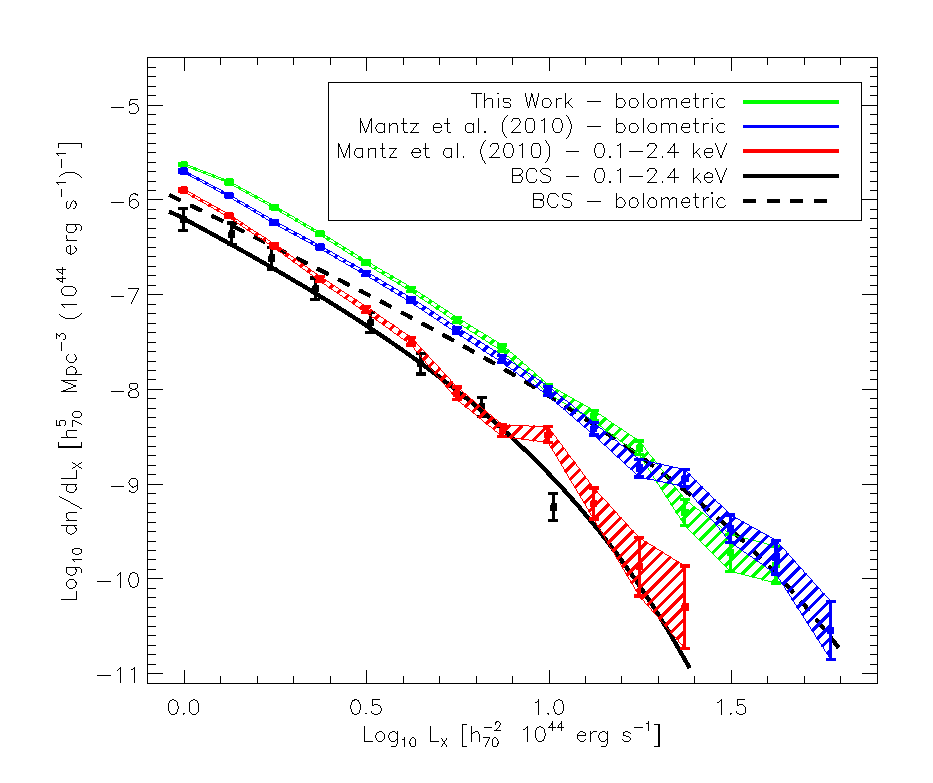
\includegraphics[width=0.48\textwidth]{figures/xlf.eps}
\caption{Bolometric and soft-band ($0.1-2.4$~keV) XLFs. Shown are the soft-band
  data points, the soft-band and bolometric Schechter fits of the BCS sample of
  \protect\cite{1997ApJ...479L.101E}, which has a median of $z \approx 0.08$.  While the
  soft-band XLF, which was obtained applying the \protect\cite{2010MNRAS.406.1773M}
  $L_{\rmn{X}}-M_{500}$ relation to the MultiDark $z = 0.1$ snapshot, compares
  well with the BCS data points, it deviates from the corresponding Schechter
  fit. We also show the bolometric XLF of \protect\cite{2010MNRAS.406.1773M} and
  bolometric XLF of our model at $z=0.1$. The XLFs are calculated in equally
  log-spaced mass bins; the error bars represent the Poissonian errors. Note
  that we limit the comparison to the luminosity range covered by our sample,
  where we cut the lowest part because in that range the XLF rapidly drops due
  to the imposed mass cut.}
\label{fig:XLF}
\end{figure}

Summarizing, our phenomenological approach provides viable gas densities that
reproduce the observed scaling relations of the ICM as well as the XLF. Thus, we
will apply it in the following to model the CR population in galaxy clusters and
to predict the hadronically induced radio and gamma-ray emission of our sample.


%%%%%%%%%%%%%%%%%%%%%%%%%%%%%%%%%%%%%%%%%%%%%%%%%%%%%%%%%%%%%%%%%%%
\subsection{Cosmic ray modeling}
\label{sec:2.3}
We assume a power-law for the spectral distribution of CR protons, $f(R,p) \dd
p=C(R) p^{-\alpha} \dd p$, which is the effective one-dimensional momentum
distribution (assuming isotropy in momentum space). We are interested in
calculating the radio synchrotron (and gamma-ray) emission resulting from
secondaries of hadronic CR interactions with protons of the ICM. To start, we
provide the synchrotron emissivity $j_{\nu}$, at frequency $\nu$ and per
steradian, of a steady-state electron population where radiative cooling
balances injection from hadronic interactions (adapted from
\citealp{2008MNRAS.385.1211P} and \citealp{2011A&A...527A..99E}),
\begin{equation}
j_{\nu}  =  A_\nu C(R) \rho_{\rmn{gas}}(R) 
\frac{\epsilon_{\rmn{B}}(R)}{\epsilon_{\rmn{B}}(R)+\epsilon_{\rmn{CMB}}} 
\left( \frac{\epsilon_{\rmn{B}}(R)}{\epsilon_{B_{\rmn{c}}}} \right)^{(\alpha-2)/4},
\label{eq:jnu}
\end{equation}
where the abbreviations $A_\nu$ and $\epsilon_{B_{\rmn{c}}}$ are defined in
Appendix~\ref{app:A}. $\epsilon_{\rmn{CMB}}$ is the energy density of the cosmic
microwave background (CMB), and $\epsilon_B=B^{2}/(8\pi)$ denotes the magnetic
energy density. We assume a scaling of the magnetic field with gas density that
is given by
\begin{equation}
B(R) = B_0\,\left(\frac{\rho_{\rmn{gas}}(R)}{\rho_{\rmn{gas},0}}\right)^{ \alpha_{\rmn{B}}},
\label{eq:B}
\end{equation}
where $B_0$ is the central magnetic field and $\alpha_{\rmn{B}}$ describes the
declining rate of the magnetic field strength toward the cluster outskirts. Such
a parametrization is suggested by cosmological simulations
\citep{2008A&A...482L..13D} as well as Faraday rotation measurements \citep[][and
references therein]{2010A&A...513A..30B, 2011A&A...529A..13K}.  The radio
surface brightness $S_{\nu}(R_{\perp})$ (in the small-angle approximation) and
luminosity $L_{\nu}$, at a given frequency $\nu$, are given by
\begin{eqnarray}
S_\nu(R_{\perp}) &=& 2 \int_{R_{\perp}}^{\infty} j_{\nu}(R) \frac{R}{\sqrt{R^{2}-R_{\perp}^{2}}} \rmn{d}R, \label{eq:surf} \\
L_{\nu}  &=&  4 \pi \int \dd V j_\nu(R).
\label{eq:lum}
\end{eqnarray}
The flux is given by $F_{\nu}=L_{\nu}/(4\pi D^{2})$ where $D$ is the luminosity
distance to the object. Note that we do not convolve $S_\nu$ with the instrumental
point spread function unless specified.

The spatial CR distribution within a galaxy cluster is governed by an interplay
of CR advection, streaming, and diffusion. The advection of CRs by turbulent gas
motions is dominated by the largest eddy turnover time $\tau_{\rmn{tu}}\sim
L_{\rmn{tu}}/ \vel_{\rmn{tu}}$. Here, $L_{\rmn{tu}}$ denotes the turbulent
injection scale (typically of order the core radius) and $\vel_{\rmn{tu}}$ is
the associated turbulent velocity that approaches the sound speed
$\vel_{\rmn{s}}$ for transsonic turbulence after a cluster merger and relaxes to
small velocities afterwards. As a result of advection into the dense cluster
atmosphere, CRs are adiabatically compressed and experience a stratified
distribution in the cluster potential. The gradient of the CR number density
leads to a net CR streaming motion towards the cluster outskirts. Streaming CRs
excite Alfv{\'e}n waves on which they resonantly scatter
\citep{1969ApJ...156..445K}. This isotropizes the CRs' pitch angles, and thereby
reduces the CR bulk speed. Balancing the growth rate of the CR Alfv{\'e}n wave
instability with the wave damping rate due to non-linear Landau damping yields a
CR streaming speed of order the Alfv{\'e}n speed \citep{2001ApJ...553..198F}.
This increases considerably when balancing it with the turbulent damping rate,
which implies an inverse scaling with the CR number density (Wiener, Oh \& Guo,
in prep). Once CR streaming depletes the CR number density, this causes a
run-away process with a rapidly increasing streaming speed that even surpasses
the sound speed because the smaller CR number density drives the CR Alfv{\'e}n
wave instability less efficiently. Hence, the crossing time of streaming CRs
over $L_{\rmn{tu}}$ is $\tau_{\rmn{st}}\sim \chi_B\,L_{\rmn{tu}}/
\vel_{\rmn{st}}$ with the streaming velocity given by $\vel_{\rmn{st}}\sim
\vel_{\rmn{s}}$ and $\chi_B\lesssim 1$ parametrizes the magnetic bending scale.
Magnetic bottlenecks for the macroscopic, diffusive CR transport, are critical
in lowering the microscopic streaming velocity of CR by some finite
factor. Therefore, we can define a turbulent propagation parameter
\begin{equation}
  \label{eq:gamma_tu}
  \gamma_{\rmn{tu}}\equiv\frac{\tau_{\rmn{st}}}{\tau_{\rmn{tu}}}=
  \frac{\chi_B\,\vel_{\rmn{tu}}}{\vel_{\rmn{st}}}
\end{equation}
that indicates the relative importance of advection versus CR streaming as the
dominant CR transport mechanism. After a merger, turbulent advective transport
dominates yielding $\gamma_{\rmn{tu}}\gg 1$, which results in centrally enhanced
CR profiles. In contrast, in a relaxed cluster, CR streaming should be the
dominant transport mechanism implying $\gamma_{\rmn{tu}}\sim1$ and producing
flat CR profiles (for a detailed discussion of these processes, see
\citealp{2011A&A...527A..99E}).

We propose here to take the spectral shape of the CR distribution function from
cosmological hydrodynamical simulation of clusters \citep{2010MNRAS.409..449P},
which however did not account for CR streaming. Hence the spatial CR
distribution has to be modified to include the effects of CR streaming. For this
reason we adopt the analytical result from \citet{2011A&A...527A..99E}. This
yields a model that includes the necessary CR transport physics and is able to
predict the radio and gamma-ray emission while reproducing the observed RH
properties. Note that this approach is not fully self-consistent and points to
the necessity of future hydrodynamical simulations to include the effect of CR
streaming and diffusion on the CR spectrum.

\begin{figure*} 
\centering
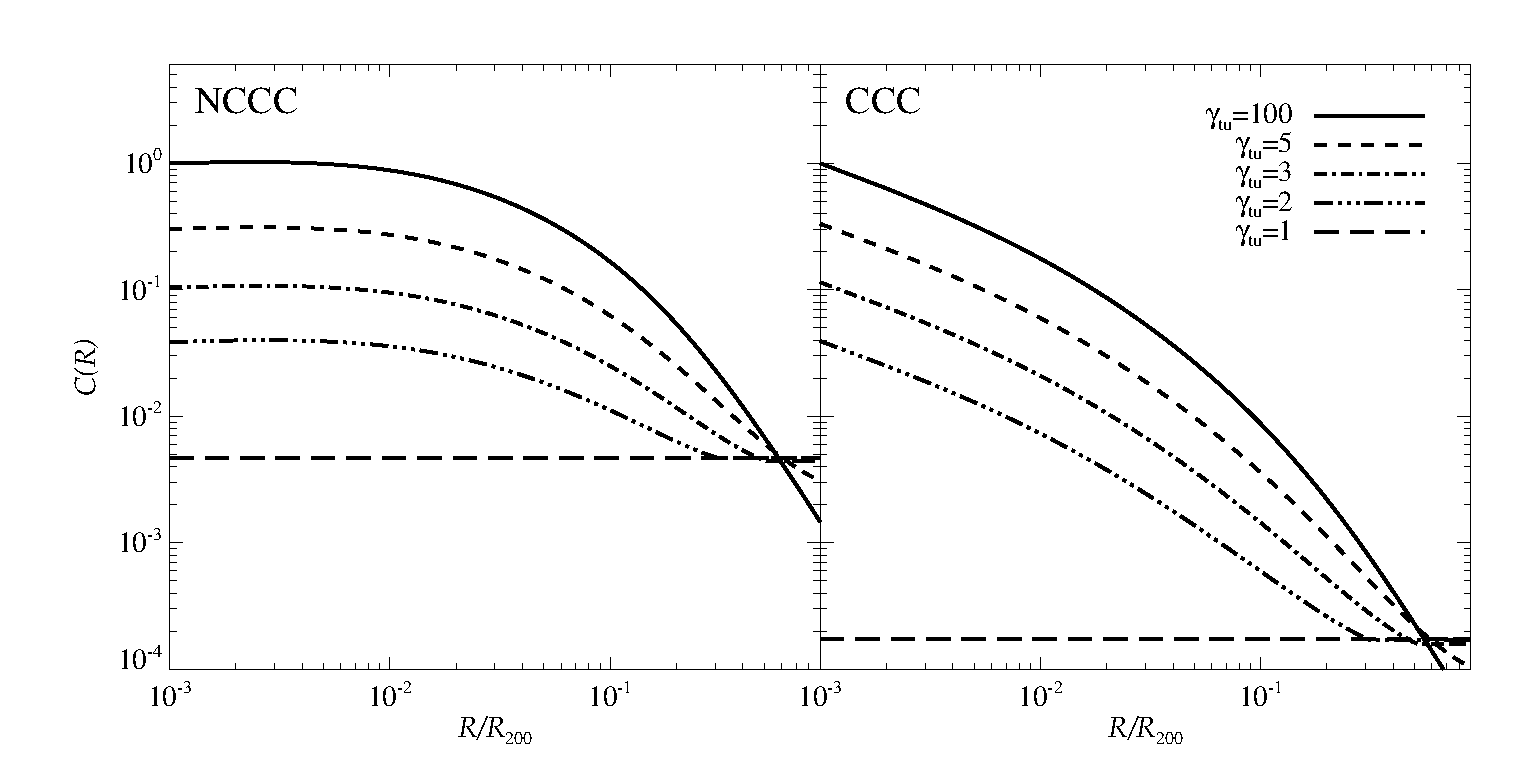
\includegraphics[width=0.62\textwidth]{figures/CR_profiles_FinalModel.eps}
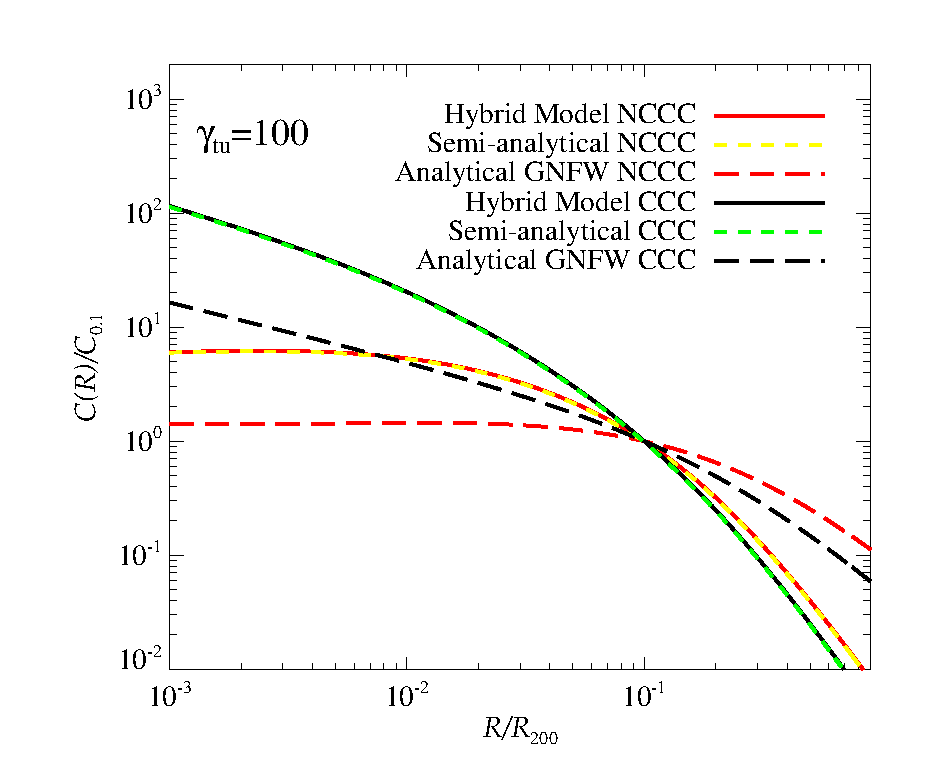
\includegraphics[width=0.37\textwidth]{figures/CR_profiles_FinalModelvsREX_norm0.1.eps}
\caption{\emph{Left panel.} We show our extended model profiles for the
  normalization of the CR distribution for the NCCC and CCC cases and for
  different values of $\gamma_{\rmn{tu}}$. We fix the CR number for the case of
  $\gamma_{\rmn{tu}}=100$ using equation~(36) of \protect\cite{2011A&A...527A..99E},
  while integrating the cluster volume within $R_{200}$, and require CR number
  conservation during CR streaming. \emph{Right panel.} We compare the
  extended model (adopting $\gamma_{\rmn{tu}}=100$) with the semi-analytical
  advection-only case (adopting our GNFW gas profiles and the outer temperature
  decrease to the simulation-derived model proposed by
  \protect\citealp{2010MNRAS.409..449P}) and with the exact analytical solution as in
  \protect\citet{2011A&A...527A..99E}, but for our GNFW profiles (adopting $\alpha=2.3$
  and $\gamma_{\rmn{tu}}=100$). Here, the CR profiles are normalized at
  $C_{0.1}=C(0.1R_{200})$.}
\label{fig:CRFinalModel}
\end{figure*}

To construct such a model, we have to generalize the approach proposed by
\citet{2011A&A...527A..99E} in order to account for GNFW gas profiles
(Section~\ref{sec:2.2}). We also have to include the cluster mass-scaling of the
CR normalization obtained from simulations \citep{2010MNRAS.409..449P}. While
details are given in Appendix~\ref{app:B}, we show below the main steps. When
turbulent advection completely dominates the CR transport, the CR normalization
can be written as \citep{2011A&A...527A..99E}
\begin{equation}
C_{\rmn{adv}}(R)=C_{0} \left( \frac{P_{\rmn{th}}(R)}{P_{\rmn{th},0}} \right)^{\frac{\beta_{\rmn{CR}}}{\gamma}} = 
C_{0} \eta(R)^{\beta_{\rmn{CR}}},
\label{eq:Csimple_1}
\end{equation} 
where $\beta_{\rmn{CR}}=(\alpha+2)/3$, $\gamma=5/3$, and we introduced the
advective CR profile $\eta(R)=(P(R)/P_0)^{1/\gamma}$. Solving the continuity
equation for CRs, \citet{2011A&A...527A..99E} derive the CR density profile,
\begin{equation}
\rho_{\rmn{CR}}(R) = \rho_{\rmn{CR},0} \eta(R) \rmn{exp} \left( \frac{R}{R_{*}} \right) \, ,
\label{eg:rhoCR_1}
\end{equation} 
where $R_{*}=\gamma_{\rmn{\rmn{tu}}}R_{\rmn{c}}$ and $R_{\rmn{c}}$ is the characteristic 
radius, of order the core radius, at which the turbulence is supposed to be injected.
Now, we introduce the \emph{semi-analytical} mass-dependent normalization of the
CR profile of \cite{2010MNRAS.409..449P} such that
\begin{equation}
\eta(R) = \left( \frac{C_{\rmn{adv}}(R)}{C_0} \right)^{1/\beta_{\rmn{CR}}} \to
\left( \frac{C_{\rmn{extended}}(R)}{C_0} \right)^{1/\beta_{\rmn{CR}}} \, ,
\label{eq:eta}
\end{equation} 
which effectively redefines $C_{\rmn{adv}}(R)$ by that of our extended model, i.e.,
\begin{equation}
C_{\rmn{extended}}(R) =  \tilde{C}(R)\, \frac{\rho_{\rmn{gas}}(R)}{m_\rmn{p}} \frac{T(R)}{T_0}.
\label{eq:Cf}
\end{equation} 
Here, $\tilde{C}(R)$ is the normalization CR profile of equation~(22) of
\cite{2010MNRAS.409..449P}. We additionally account for the temperature
decline toward the cluster periphery, $T(R)$, given by the fit to the universal
temperature profile obtained from cosmological hydrodynamical simulations
\citep{2007MNRAS.378..385P,2010MNRAS.409..449P} and deep {\em Chandra} X-ray
observations \citep{2005ApJ...628..655V}. Eventually, the CR profile in our
extended model is $C(R)=C_{0}(\rho_{\rmn{CR}}(R) /
\rho_{\rmn{CR},0})^{\beta_{\rmn{CR}}}$ within $R_{\pm}$ of
equation~(\ref{eq:Rpm}), with $\rho_{\rmn{CR}}$ defined by
equation~(\ref{eg:rhoCR_1}) where $C_{\rmn{extended}}$ enters through our
redefinition of $\eta$, and $C(R) = C(R_{\pm})$ for $R > R_{+}$ and $R < R_{-}$,
respectively.

The last step is to generalize the case of one CR population with a single
spectral index $\alpha$ to include the spectral curvature as suggested by
\cite{2010MNRAS.409..449P}. They model the CR spectrum with three different
power-law CR populations with spectral indices of
$\alpha_{i}=(2.15,2.3,2.55)$. Our formalism can be easily extended to account
for multiple CR populations by extending the terms with a single $\alpha$ to
sums over the three spectral indices (\citealp{2010MNRAS.409..449P}). This
extension has to be applied to $A_{\nu}$, to the factor $(\epsilon_{\rmn{B}}(R)/
\epsilon_{B_{\rmn{c}}})^{(\alpha-2)/4}$ of equation~(\ref{eq:jnu}), and to
equation~(\ref{eq:Csimple_1}). While the modifications are straight forward in
the first two cases (and are adopted for our extended model,
Appendix~\ref{app:A}), introducing a sum over $\alpha_{i}$ in
equation~(\ref{eq:Csimple_1}) would make impossible to solve analytically for
$\eta(R)$ in equation~(\ref{eq:eta}). For simplicity, we decided to only use
$\alpha = 2.3$ in this last case.\footnote{We checked that the choice of
  $\alpha$ in equation~(\ref{eq:Csimple_1}) has only a minor effect on the
  results. Varying $\alpha$ within $2.15-2.55$ leaves the radial shape and the
  normalization unchanged within $0.5\%$.} For the highly turbulent cases, i.e.,
for $\gamma_{\rmn{tu}}=100$ (1000), we recover the radial shape and
normalization of the semi-analytical model of \cite{2010MNRAS.409..449P} within
$1\%$ ($0.1\%$).

Summarizing, our \emph{extended} model for the CR distribution function, has the
following properties: it accounts for (i) the X-ray-inferred (CCC and NCCC) gas
profiles and cluster-mass scaling of the gas fraction, in addition to the
universal temperature drop in the outskirts of clusters, (ii) a cluster-mass
dependent CR normalization and universal CR spectrum as derived from
cosmological hydrodynamical simulations, (iii) an effective parametrization of
active CR transport processes, including CR streaming and diffusion, which
allows us to explore different turbulent states of the clusters in our MultiDark
sample.

In the left two panels of Fig.~\ref{fig:CRFinalModel}, we show our extended CR 
normalization for the NCCC and CCC cases and for different values of
$\gamma_{\rmn{tu}}$.  As expected, when CR streaming is the dominant CR
transport mechanism, i.e., for negligible advective turbulent transport or
equivalently, $\gamma_{\rmn{tu}}\sim1$, the spatial CR profiles are flattened
irrespective of the cluster state. While turbulence in NCCCs could be
injected by a merging (sub-)cluster, in the case of CCCs, the interaction of the
AGN jet or radio lobe with the ambient ICM could be the source of turbulence.

In the right panel of Fig.~\ref{fig:CRFinalModel}, we compare our extended model
profile with the semi-analytical advection-only case (adopting our GNFW gas
profiles and the outer temperature decrease to the model proposed by
\citealp{2010MNRAS.409..449P}) and with the exact analytical solution as in
\citet{2011A&A...527A..99E}, but for our GNFW profiles (Appendix~\ref{app:B}
for details).  The profiles are normalized at $0.1 R_{200}$. In that case of
dominant advective CR transport, our extended model compares nicely with the
semi-analytical model derived from cosmological cluster simulations
\citep{2010MNRAS.409..449P}.  The main differences between our extended model (and
the semi-analytical model) on the one side and the analytical solution on the
other side is the inclusion of the simulation-based ``reference'' profile
$\tilde{C}$ for the advection-only case and the universally observed temperature
drop towards the outskirts of clusters. Note that the profiles in our extended
model are generally more centrally peaked in comparison to the analytical GNFW
case, which is due to the enhanced radiative cooling in the
\citet{2010MNRAS.409..449P} simulations that did not account for AGN
feedback. Thanks to the flexible parametrization in our model, this can be
easily counteracted by changing $\gamma_{\rmn{tu}}$ and $ \alpha_{\rmn{B}}$, however, at
the expense that these parameters are now degenerate with our assumptions on the
CR profile in the advection-dominated regime and other possible effects that we
are not considering such as cluster asphericity (see also next
Section~\ref{sec:3}).


%%%%%%%%%%%%%%%%%%%%%%%%%%%%%%%%%%%%%%%%%%%%%%%%%%%%%%%%%%%%%%%%%%%
%%%%%%%%%%%%%%%%%%%%%%%%%%%%%%%%%%%%%%%%%%%%%%%%%%%%%%%%%%%%%%%%%%%
\section{Radio Surface Brightness Modeling}
\label{sec:3}

In this Section, we apply our model to reproduce the emission characteristics of
four well-observed RHs. Hence for the purpose of this section, we adopt the
measured gas and temperature profiles derived from X-ray observations of each cluster.  
Our extended model includes an overall normalization $g_{\rmn{CR}}$ of the CR
distribution function and the hadronically-induced non-thermal emission 
(Appendix~\ref{app:A}). Note that
this parameter can be interpreted as a functional that depends on the
\emph{maximum CR acceleration efficiency}, $g(\zeta_{\rmn{p,max}})$,
\citep{2010MNRAS.409..449P} but \emph{only} for
$\gamma_{\rmn{tu}}\gtrsim100$. We will additionally study the CR-to-thermal
pressure $X_{\rmn{CR}}=P_{\rmn{CR}}/P_{\rmn{th}}$, where the CR pressure is
given by
\begin{equation}
  \label{eq:PCR}
  P_{\rmn{CR}}=\frac{g_{\rmn{CR}} C m_{\rmn{p}} c^{2}}{6}
  \sum_{i=1}^{3} \Delta_{i} \mathcal{B}_{1/(1+q^2)} \left(
    \frac{\alpha_{i}-1}{2},\frac{3-\alpha_{i}}{2} \right).
\end{equation}
Here, $c$ is the speed of light, $q=0.8$ is the low-momentum cutoff of the CR
distribution, and the normalization factors of the individual CR populations are
given by $\Delta_{i} = (0.767, 0.143, 0.0975)$ \citep[][see also
Appendix~\ref{app:A}]{2010MNRAS.409..449P}.

For our study, we choose the giant radio halos of Coma
\citep{1997A&A...321...55D} and Abell~2163 \citep{2001A&A...373..106F,
  2009A&A...499..679M}, both in merging NCCCs, and the radio mini-halos of
Perseus \citep{1990MNRAS.246..477P} and Ophiuchus \citep{2009A&A...499..371G,
  2009A&A...499..679M}, both in relaxed CCCs. The radio emission of these
clusters is representative of a wide class of RHs.  Additionally, Perseus,
Ophiuchus and Coma are among the most promising clusters for gamma-ray
observations \citep{2010MNRAS.409..449P,2011arXiv1105.3240P}. 
We use X-ray-inferred gas densities $\rho_{\rmn{gas}}$ and temperatures 
for Coma \citep{1992A&A...259L..31B}, for A2163 and Ophiuchus 
\citep{2002ApJ...567..716R}, and for Perseus \citep{2003ApJ...590..225C}. 
In Table~\ref{tab:RadioHalos}, we summarize the main characteristics of these RHs.

To assess the ability of our extended hadronic model to fit the observed surface
brightness profiles, we scan our physically motivated parameter
space. Generally, the normalization of the magnetic profile, $B_0$, and the CR
acceleration efficiency function, $g_{\rmn{CR}}$, determine the overall
normalization of the radio emission. The radial decline of the magnetic field,
$ \alpha_{\rmn{B}}$, and the turbulent CR propagation parameter, $\gamma_{\rmn{tu}}$, both
determine the shape of the radio profile and, hence, are also degenerate. By
scanning the allowed parameter space and asserting Bayesian priors that rely on
observational constraints and theoretical considerations about likely parameter
combinations for certain classes (mini halos versus giant halos), we will draw
conclusions on the applicability of the hadronic model for RHs.  In
Fig.~\ref{fig:SBmodeling}, we show the surface brightness and CR-to-thermal
pressure profiles of each cluster together with the allowed
$\gamma_{\rmn{tu}}-\alpha_{B}$ parameter space. All these clusters are
modeled at 1.4~GHz and within $R_{200}$, unless differently specified.

\begin{table} 
\begin{center}
\caption{Radio-halo and mini-halo characteristics.}
\medskip
%\begin{tabular}{cccccccc}
%\hline
%\phantom{\Big|}
%name & $z$ & $D$ & $\Delta d$ & $L_{1.4~\rmn{GHz},~\rmn{obs}}$ & model parameters & $L_{1.4~\rmn{GHz},~\rmn{model}}$ & references \\
%\phantom{\Big|}
%           &   & [$h_{70}^{-1}$~Mpc] & [$h_{70}^{-1}$~Mpc] & $10^{31}$ [$h_{70}^{-2}$~erg~s$^{-1}$~Hz$^{-1}$] & $\gamma_{\rmn{tu}}$, $\alpha_{\rmn{B}}$ & $10^{31}$ [$h_{70}^{-2}$~erg~s$^{-1}$~Hz$^{-1}$] & \\
%\hline \\[-0.5em]
%Coma           & $0.023$ & $101$ & $2.15$ & $0.72$  & 1, 0.6  & 0.86 &  [1, 2, 3]   \\
%               &         &       &        &                        & 4, 0.3  & 0.90  &  \\
%A2163         & $0.203$ & $962$ & $2.07$ & $15.36$     & 1, 0.3  & 13.43  &  [3, 4]  \\
%\hline \\[-0.5em]
%Perseus        & $0.018$ & $78$   & $0.15$ & $4.40$ & 3, 0.4   & 4.80 &  [3, 5, 6]  \\
%               &         &        &        &                       & 100, 0.3 & 3.97 &  \\
%Ophiuchucs     & $0.028$ & $121$  & $0.41$ & $0.19$       & 5, 0.7   & 0.19  &  [3, 4] \\
%               &         &        &        &                       & 100, 0.3 & 0.23 &   \\[0.5em]
\begin{tabular}{lcrrc}
\hline
\phantom{\Big|}
 cluster & $z$ & $D$~~ & $L_{1.4~\rmn{GHz}}$ & references \\
\hline \\[-0.5em]
Coma           & $0.023$ & $101$ & $0.72$  &  [1]   \\
A2163         & $0.203$ & $962$ & $15.36$  &  [2]  \\
\hline \\[-0.5em]
Perseus        & $0.018$ & $78$   & $4.40$ &  [3]  \\
Ophiuchucs     & $0.028$ & $121$  & $0.19$  &  [2] \\[0.5em]
\hline
\end{tabular}
\label{tab:RadioHalos}
\end{center}
\footnotesize{Note. Top two rows correspond to giant radio halos, while the
  bottom two rows are radio mini-halos.  $D$ is the luminosity distance in units
  of $h_{70}^{-1}$~Mpc and $L_{1.4~\rmn{GHz}}$ is the observed radio luminosity
  at 1.4~GHz in units of $10^{31}$~$h_{70}^{-2}$~erg~s$^{-1}$~Hz$^{-1}$.
  References: [1] \cite{1997A&A...321...55D} [2] \cite{2009A&A...499..679M} [3]
  \cite{1990MNRAS.246..477P}.}
\end{table}

\del{$M_{200}$ and $R_{200}$ are taken from \cite{2002ApJ...567..716R}. }

\begin{figure*}
\centering
%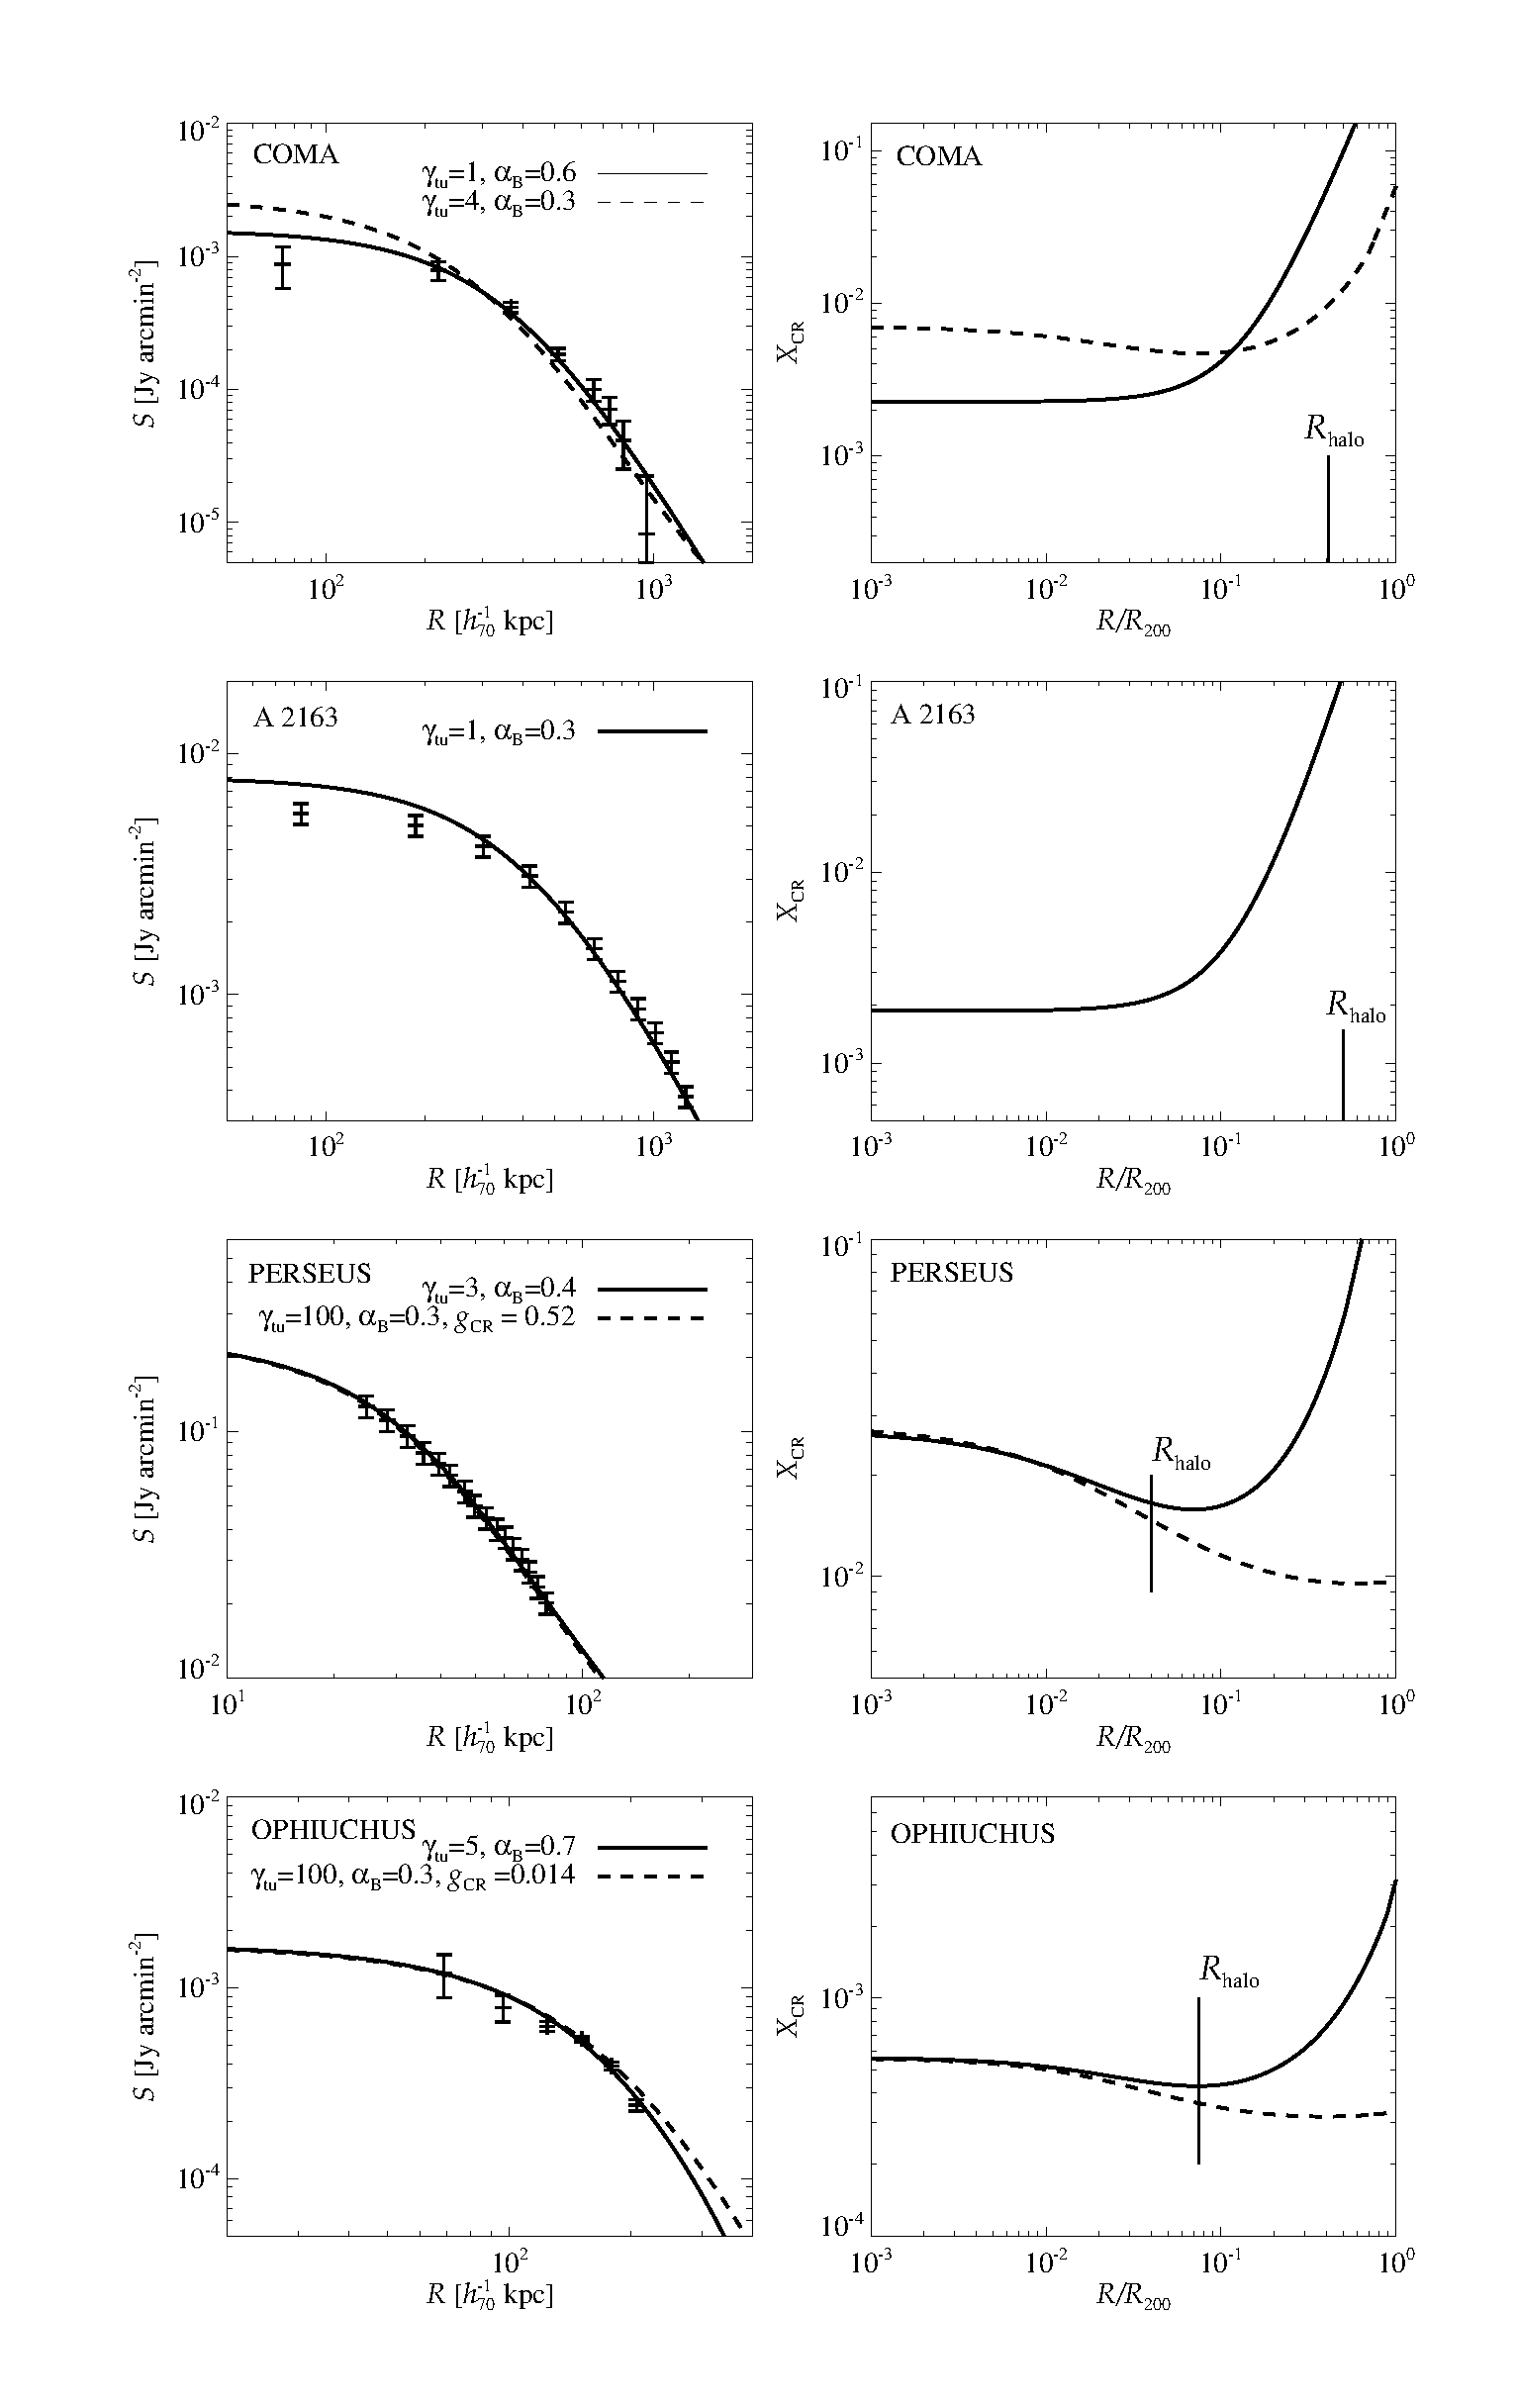
\includegraphics[width=0.75\textwidth]{figures/SB_profiles_ALL.eps}
%
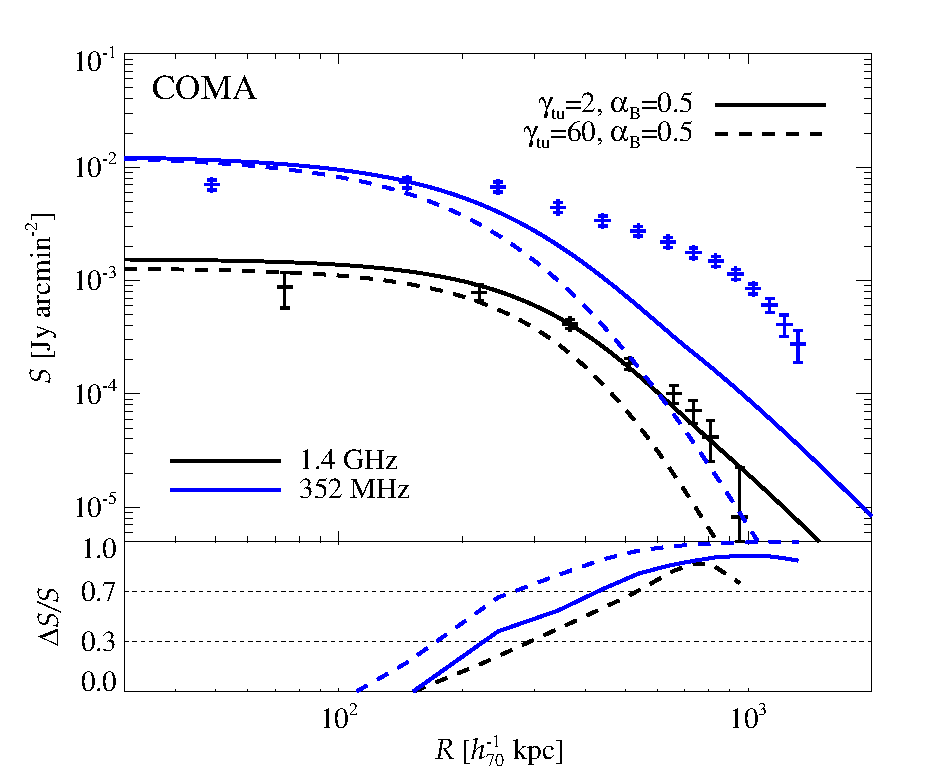
\includegraphics[width=5.5cm,height=5.5cm,keepaspectratio]{figures/SB_Coma.eps}
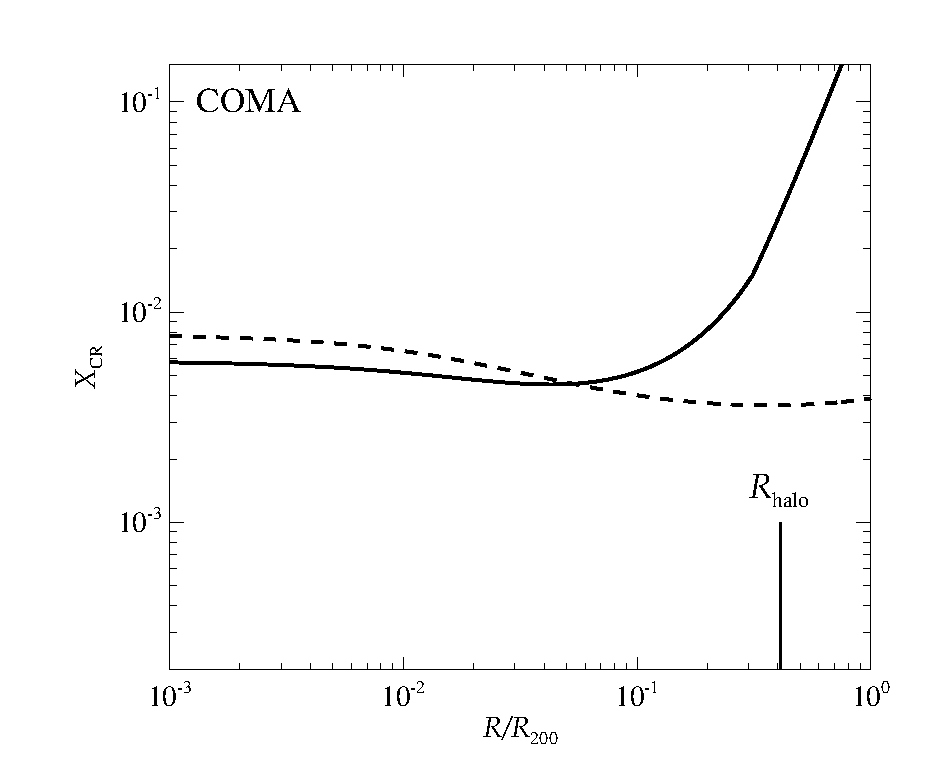
\includegraphics[width=5.6cm,height=5.6cm,keepaspectratio]{figures/XCR_Coma.eps}
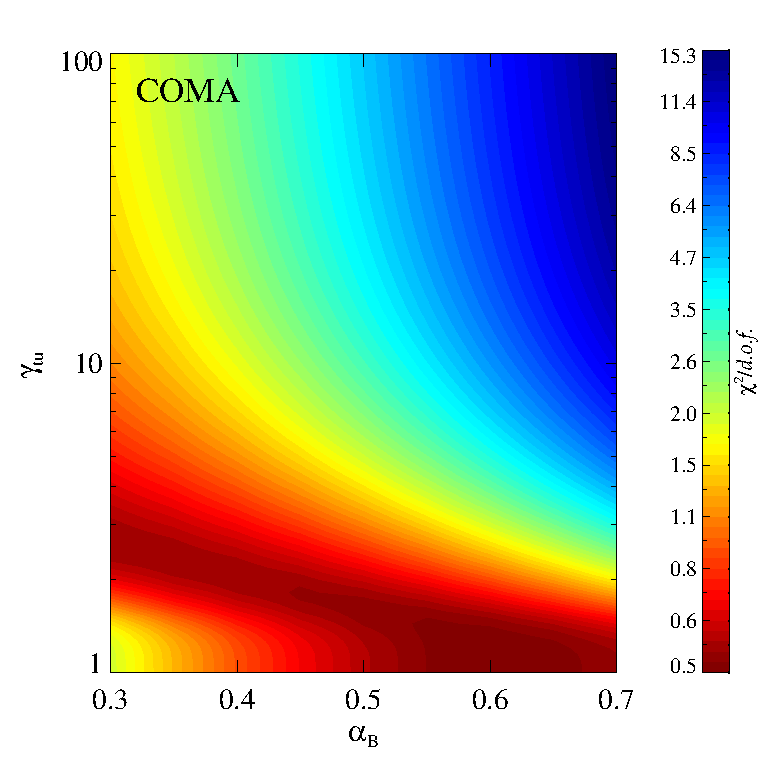
\includegraphics[width=5cm,height=4.6cm]{figures/ProbComa.eps}
%%
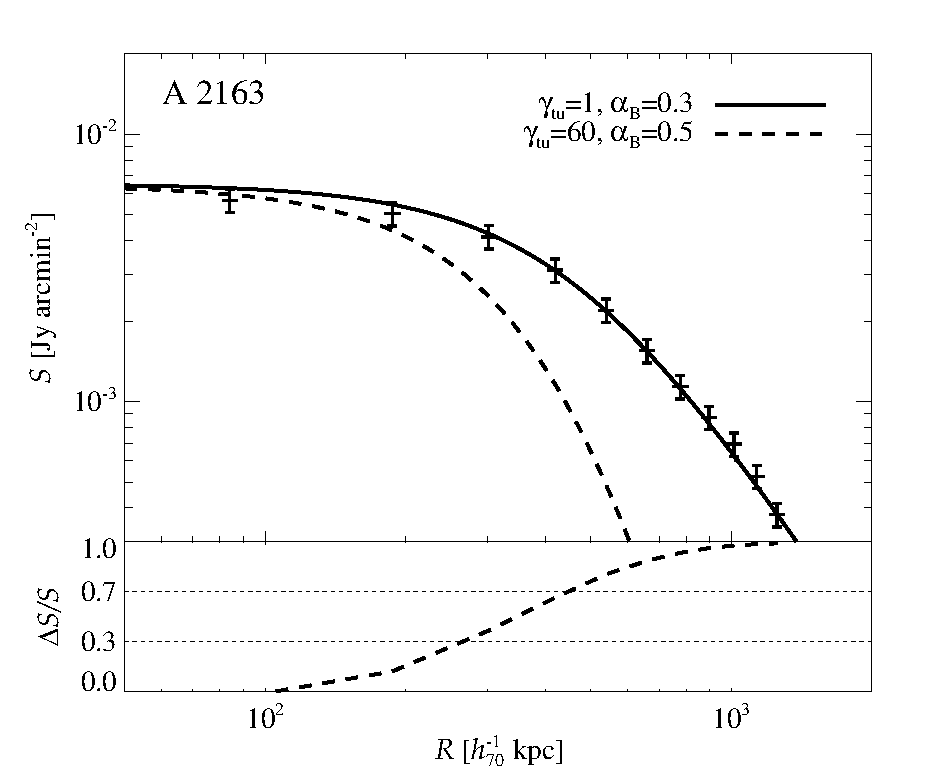
\includegraphics[width=5.5cm,height=5.5cm,keepaspectratio]{figures/SB_A2163.eps}
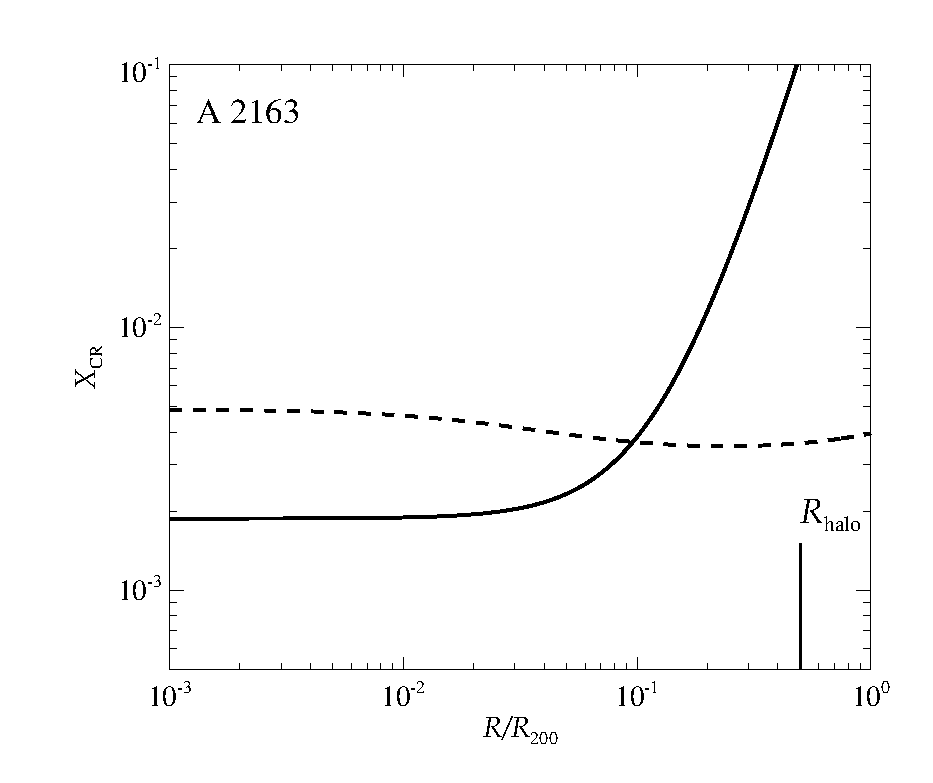
\includegraphics[width=5.6cm,height=5.6cm,keepaspectratio]{figures/XCR_A2163.eps}
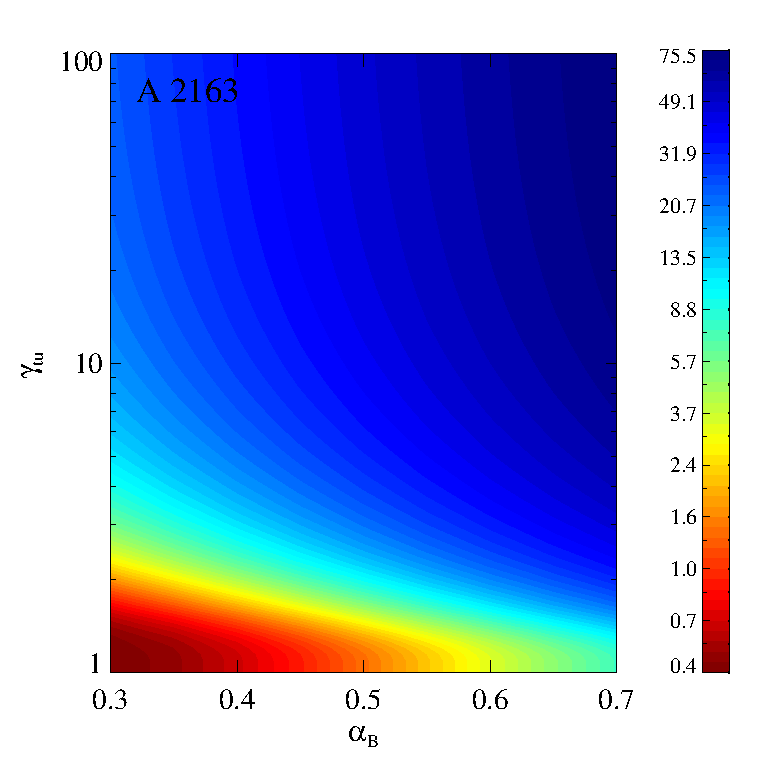
\includegraphics[width=5cm,height=4.6cm]{figures/ProbA2163.eps}
%%
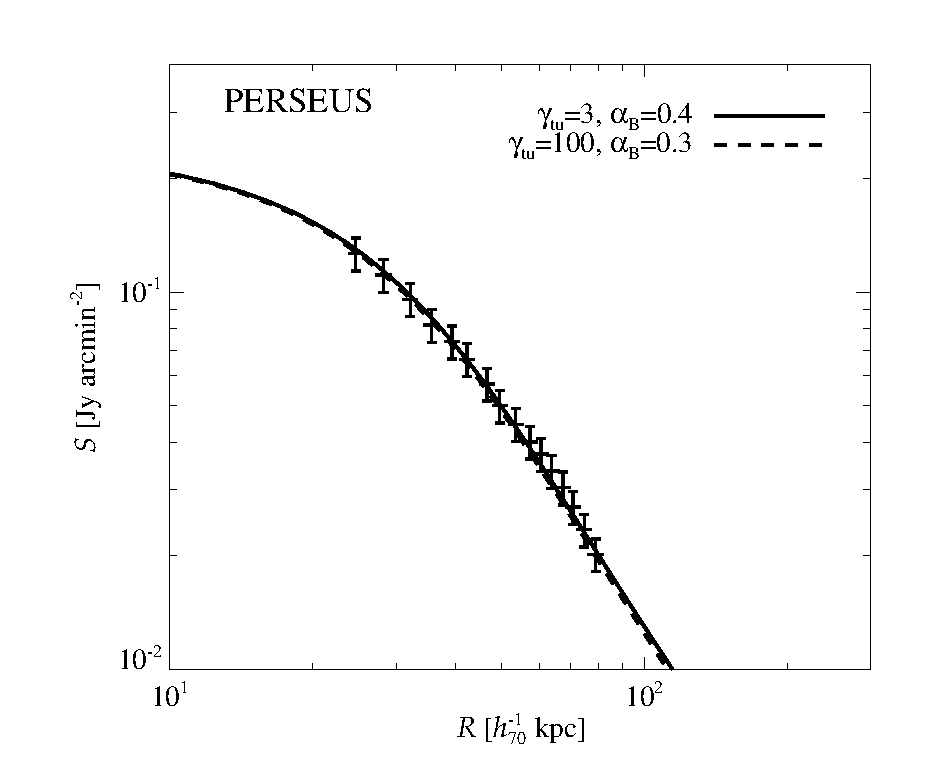
\includegraphics[width=5.6cm,height=5.6cm,keepaspectratio]{figures/SB_Perseus.eps}
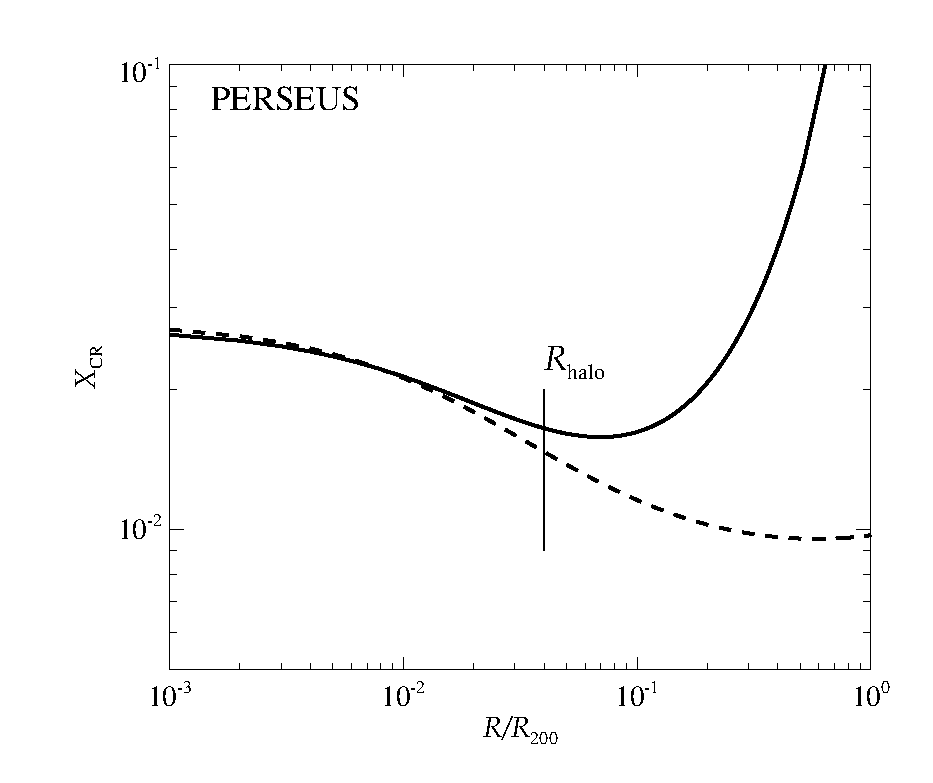
\includegraphics[width=5.6cm,height=5.6cm,keepaspectratio]{figures/XCR_Perseus.eps}
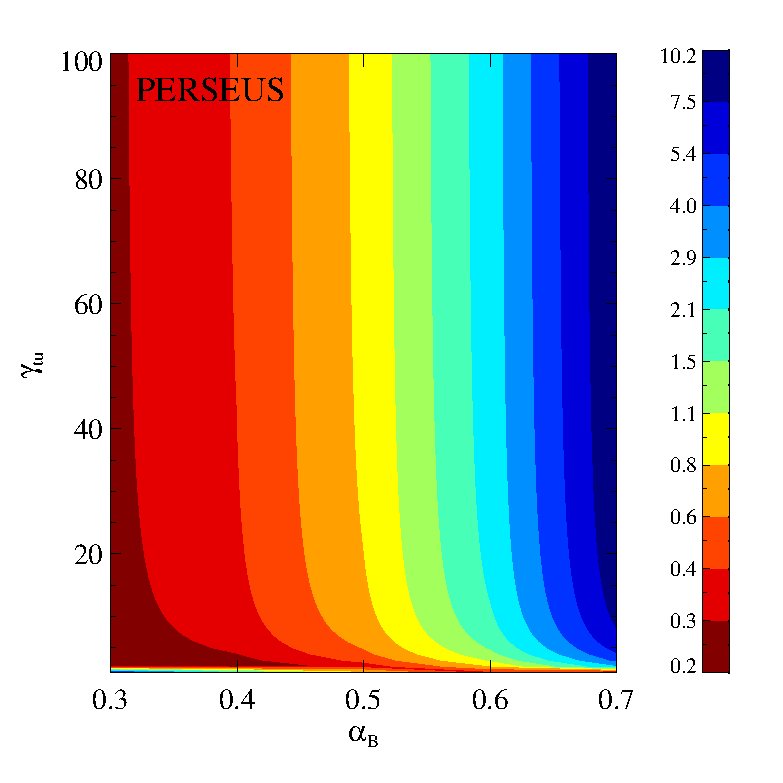
\includegraphics[width=5cm,height=4.6cm]{figures/ProbPerseus.eps}
%%
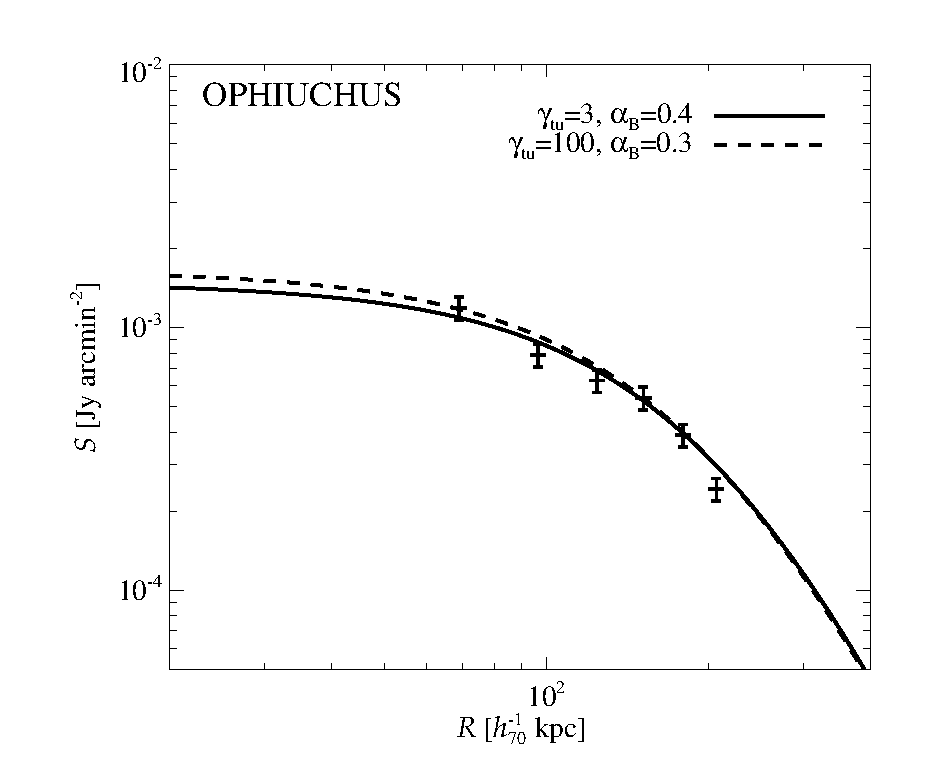
\includegraphics[width=5.6cm,height=5.6cm,keepaspectratio]{figures/SB_Ophiuchus.eps}
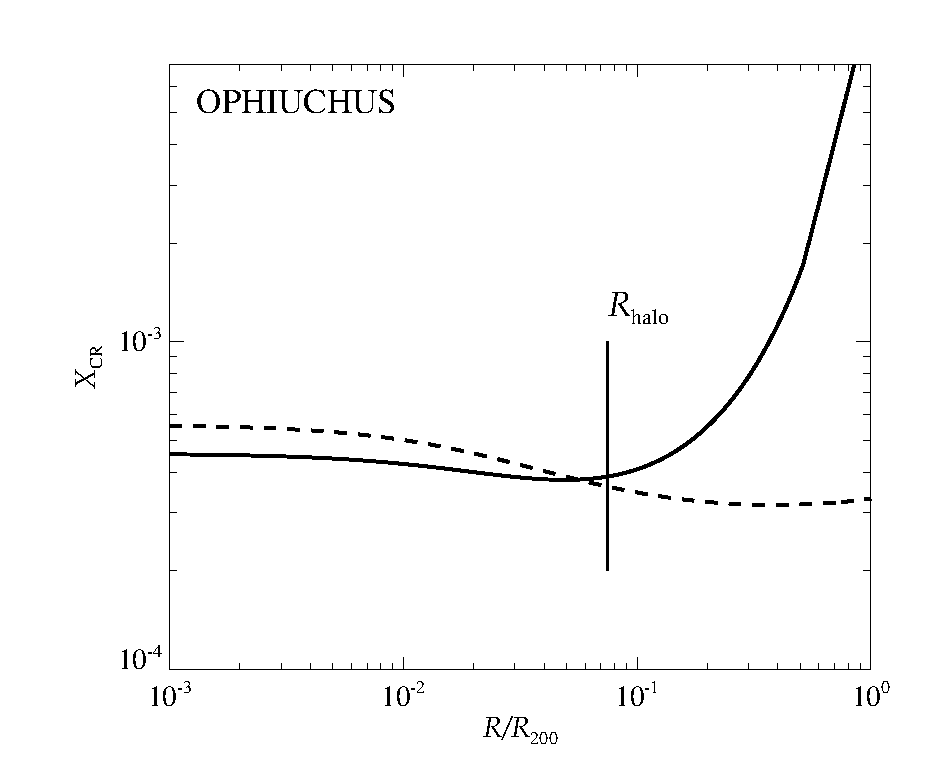
\includegraphics[width=5.6cm,height=5.6cm,keepaspectratio]{figures/XCR_Ophiuchus.eps}
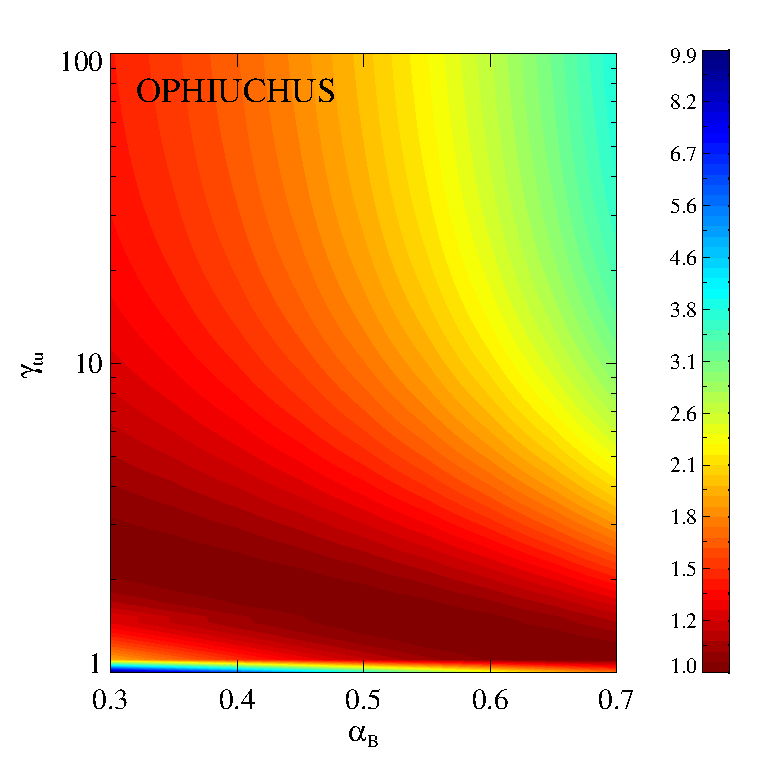
\includegraphics[width=5cm,height=4.6cm]{figures/ProbOphiuchus.eps}
%
\caption{Surface brightness modeling of the RHs in Coma, Abell~2163, Perseus and
  Ophiuchus. The left and middle panels show the RHs' azimuthally averaged
  surface brightness profiles and the corresponding CR-to-thermal pressure
  profiles $X_{\rmn{CR}}(r)$, respectively. Representative hadronic model
  parameters that fit the data well (solid) are compared to parameter choices
  that will be used in the second part of the paper (dashed, Sects.~\ref{sec:4}
  and \ref{sec:5}), which addresses RH statistics. While radio mini-halos can be
  fit by either set of parameters, for the latter choice of parameters, the
  hadronic model is not able to explain the emission in the outer parts of giant
  radio halos and would need a secondary, leptonic component (see text for
  details). This is exemplified in the lower left panels for Coma and Abell~2163
  that show the fraction of missing surface brightness for these parameter
  choices. In the middle panels, we additionally mark the RHs' radial extension
  by a vertical line. The panels on the right show the reduced-$\chi^2$ values
  of our model fits to the data in the $\gamma_{\rmn{tu}}-\alpha_{B}$ parameter
  space. (For Coma, it refers to the 1.4~GHz case only.)  Regions of parameter
  space with reduced-$\chi^2$ values substantially larger than unity are
  excluded by the data while values much smaller than unity may point to an
  overestimate of the uncertainty intervals. Note that different parameter
  values that yield almost the same surface brightness profile may result in
  very different $X_{\rmn{CR}}$ profiles. In the case of Abell~2163 and
  Ophiuchus, we adopt a $10\%$ uncertainty range instead of the errors reported
  by \citet{2009A&A...499..679M} to account for additional systematic
  uncertainties, e.g., residual point source contamination. For Perseus, we show
  the mini-halo data only for the range that is unaffected by residual point
  sources \citep{1990MNRAS.246..477P} and adopt $10\%$ uncertainty budget.}
\label{fig:SBmodeling}
\end{figure*}


\del{ We adopt a $10\%$ uncertainty range for the inner points of the Coma
  $352$~MHz data.}

\subsection{The Coma radio halo}

The giant radio halo in Coma has a morphology remarkably similar to the extended
X-ray thermal bremsstrahlung emission, although the radio emission declines more
slowly towards the cluster outskirts \citep{1992A&A...259L..31B,
  1997A&A...321...55D}. The morphology is non-spherical, showing an elongation
in the East-West direction.  The full-width half maximum (FWHM) of the radio
beam is $0.156$~deg \citep{1997A&A...321...55D}, almost two orders of magnitude
larger than the X-ray observation of \cite{1992A&A...259L..31B}.\footnote{The
  apparent displacement of the radio and X-ray peak of about $0.05$~deg is well
  within the angular resolution of the radio observation and hence negligible
  for the modeling.}  Thus, we apply a Gaussian smoothing to our theoretical
surface brightness of equation~(\ref{eq:surf}) with $\sigma_{\rmn{smoothing}} =
FWHM_{\rmn{radio}}/2.355$.

We investigate different values for $\alpha_{\rmn{B}}\in [0.3,0.7]$ and
$\gamma_{\rmn{tu}}\in [1,100]$. First, we determine the CR number for
$\gamma_{\rmn{tu}}=100$ using equation~(36) of \cite{2011A&A...527A..99E} while
integrating the cluster volume within $R_{200}$. Then, we require CR number
conservation during CR streaming (for CR energies $E>$~GeV where Coulomb cooling
is negligible for CR protons), which is realized in our model by lowering the
values of $\gamma_{\rmn{tu}}$. Fixing the central magnetic field
$B_{0}=5$~$\mu$G \citep{2010A&A...513A..30B}, we use $g_{\rmn{CR}}$ as
normalization factor to match the radio observations.  The study of the
$\gamma_{\rmn{tu}}-\alpha_{B}$ parameter space shown in
Fig.~\ref{fig:SBmodeling} (top right panel) demonstrates the necessity of low
values of $\gamma_{\rmn{tu}}$ to match the data, i.e., very flat CR profiles. An
example of such a good match to the data is obtained for $\gamma_{\rmn{tu}}=2$
and $\alpha_{\rmn{B}}=0.5$ (top left panel). Values as high as
$\gamma_{\rmn{tu}} \approx 4$ still provide a good fit, however, at the expense
of a shallower decline of the magnetic field profile (smaller $ \alpha_{\rmn{B}}$) as a
function of cluster-centric radius. With such values, we can recover the shape
of the radio surface brightness as well as the total radio luminosity with a
maximal relative deviation of about $25\%$.

The gamma-ray flux (Appendix~\ref{app:C}) within $R_{200}$ for the parameter
combination $\gamma_{\rmn{tu}} = 2$ and $\alpha_{\rmn{B}}=0.5$ and for energies
above 100~MeV (100~GeV) is $F_{\gamma} = 2.4 \times 10^{-9}$ ($8.7 \times
10^{-13}$) cm$^{-2}$~s$^{-1}$. This is below the the gamma-ray limit recently
set with the \emph{Fermi} data of $F_{\gamma, UL} (>100~\rmn{MeV}) \approx 3.2
\times 10^{-9}$~cm$^{-2}$~s$^{-1}$ \citep{2012...VERITAS}.  Note that for
slightly higher values of $\gamma_{\rmn{tu}}$, i.e., a more centrally
concentrated CR distribution, the radio and gamma-ray yield would be increased
(assuming CR number conservation). However, in order to match the observed radio
synchrotron profiles, we have to decrease the CR normalization (parametrized by
$g_{\rmn{CR}}$). This causes the associated gamma-ray flux also to be reduced to
a level that is low enough to easily circumvent the gamma-ray constraints. E.g.,
for the parameter combination $\gamma_{\rmn{tu}} = 3$ and
$\alpha_{\rmn{B}}=0.4$, we obtain $F_{\gamma} (>100~\rmn{MeV}) = 1.3 \times
10^{-9}$~cm$^{-2}$~s$^{-1}$ (and $F_{\gamma} (>100~\rmn{GeV}) = 4.9 \times
10^{-13}$~cm$^{-2}$~s$^{-1}$).  We caution that in principle, CR streaming
should cause the CR spectrum to steepen.  This may then considerably weaken
these constraints as a result of the convex spectral curvature since the
gamma-ray emission probes the high-energy tail of the CR distribution that is
suppressed in this picture in comparison to the lower-energy protons that the
radio emission is sensitive to \citep[see][for an extended discussion of this
point]{2011arXiv1111.5544M}.

However, such low values of $\gamma_{\rmn{tu}}$ challenge the emerging picture
that only clusters that are characterized by a highly turbulent state can host
giant radio halos. For illustration, in Fig.~\ref{fig:SBmodeling}, we
additionally show the radio surface brightness for $\gamma_{\rmn{tu}} = 60$ and
$\alpha_{\rmn{B}}=0.5$ Clearly, the hadronic model is not able to explain the
emission in the outer halo parts and would need a secondary component to fill in
the `missing' hadronic radio emission.  This is exemplified in the lower plot of
the top left panel of Fig.~\ref{fig:SBmodeling}, which shows the fraction of
missing surface brightness as a function of radius and accumulates to a total
missing power of about 35\%.

Recently, \citet{2012arXiv1207.3025B} point out problems of the hadronic model
for the {\em limited} parameter space $\alpha\gtrsim2.6$, while adopting a much
broader azimuthally averaged radio halo profile at 352 MHz
\citep{2011MNRAS.412....2B} than the one used in the present study so far
\citep{1997A&A...321...55D}. The problem is only somewhat mitigated when
considering the entire parameter space of $\alpha$. In fact, harder CR spectra
of $2.1\lesssim \alpha\lesssim2.5$ provide a good description of the radio
emission after taking into account the negative flux bowl due to the SZ effect
that causes the measured radio halo spectrum to experience a sharp cutoff
towards high frequencies \citep{2004A&A...413...17P}. Hence, we complement our
RH modeling at high frequencies (1.4 GHz) with modeling of the new data at 352
MHz \citep{2011MNRAS.412....2B}. To this end, we use a {\em novel} $352$~MHz
surface brightness profile that was corrected for residual point-source
contamination by applying adaptive filtering techniques as well as adopting the
X-ray center (Rudnick, priv.{\ }comm.). The resulting profile is shown in dark
blue in the top left panel of Fig.~\ref{fig:SBmodeling} and declines somewhat
faster towards the outskirts that the profile used by
\citet{2012arXiv1207.3025B} that was not fully corrected for point-source
contamination. Nevertheless, the point-source corrected profile at 352 MHz
\citep{2011MNRAS.412....2B} is still considerably more extended than the 1.4 GHz
profile \citep{1997A&A...321...55D}.  As shown in Fig.~\ref{fig:SB_Coma}, the
1.4-GHz profile can be brought into agreement with the low-frequency profile by
choosing a lower zero level (Rudnick, priv. comm.), however at the expense of
emerging super cluster emission from the Coma region on scales much more
extended than the radio halo \citep{2007ApJ...659..267K}. Conversely, by
increasing the zero level of the 352 MHz data \citep{2011MNRAS.412....2B}
reconciles that profile with the narrower profile of \citet{1997A&A...321...55D}
(Fig.~\ref{fig:SB_Coma}), possibly at the expense of an implausibly high zero
level, judging from the more sensitive 352 MHz data (Rudnick, priv.{\ }comm.).
Assuming for a moment that the choices of zero level at both frequencies were
indeed correct, this would imply a larger extent of the radio halo at lower
frequencies. A combination of better data at 1.4 GHz, careful cleaning of the
emission of tailed radio galaxies, and a full accounting of the resulting
systematic uncertainties into the total error budget are certainly needed to
fully clarify the observational situation.

\begin{figure} 
\centering
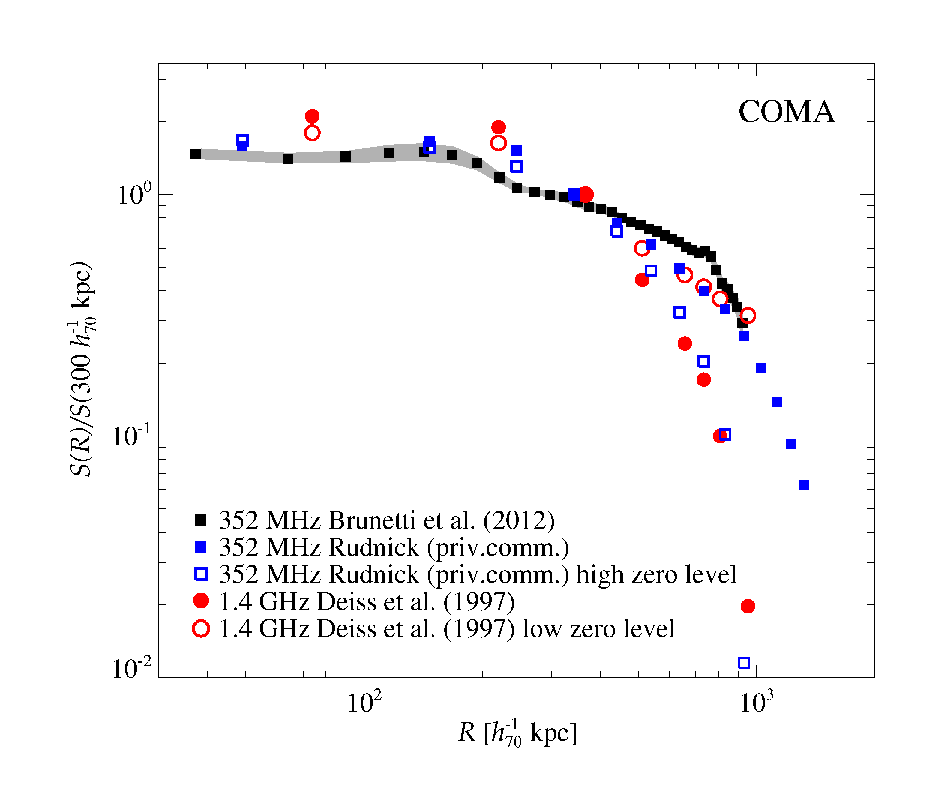
\includegraphics[width=\columnwidth]{figures/SB_Coma_norm_band.eps}
\caption{Surface brightness profiles of the Coma radio halo, normalized at 300
  kpc. We compare the 352 MHz profile of \citet{2012arXiv1207.3025B}, that is
  affected by residual point source contributions (black squares), to profiles
  where an adaptive filtering technique was applied to remove residual point
  sources (blue squares, Rudnick, priv. comm.). Increasing the zero level of the
  (more sensitive) 352 MHz data (blue open squares) to the level of 1.4 GHz halo
  data \citep[red filled circles,][]{1997A&A...321...55D} brings those data into
  agreement. Alternatively, lowering the zero level of the 1.4 GHz data (red
  open circles, Rudnick, priv. comm.) allows to match the much larger radial
  extend of the low-frequency data. Those systematic uncertainties need to be
  carefully addressed in future observations and accounted for in the error
  budget that currently only account for statistical uncertainties (grey shaded
  band, \citealp{2012arXiv1207.3025B}).}
\label{fig:SB_Coma}
\end{figure}

As shown by the 2 model realizations in Fig.~\ref{fig:SBmodeling}, the
(extended) hadronic model cannot account for the total emission at $352$~MHz for
any value in the ($\gamma_{\rmn{tu}}$, $\alpha_{\rmn{B}}$) parameter space; in
agreement with the findings of \citet{2012arXiv1207.3025B}. At the same time,
our analysis also confirms the result by \citet{2012...VERITAS} who also
conclude that the hadronic model for the Coma radio halo is a viable explanation
for magnetic field estimates inferred by Faraday rotation measure studies
\citep{2010A&A...513A..30B} and is not challenged by {\em Fermi} upper limits on
the gamma-ray emission. However, this model agreement is bought at the expense
of flat CR profiles (i.e., {\em low} $\gamma_{\rmn{tu}}$ values) that are
contrary to the expectation of turbulent clusters to host giant radio halos
(i.e., {\em high} $\gamma_{\rmn{tu}}$ values) as proposed by
\citet{2011A&A...527A..99E}. This finding hints at the necessity of a secondary,
leptonic component (within the general framework of the hadronic model) that
fills in the patchier emission in the peripheral, low-surface brightness regions
of the halo, in particular at low frequencies \cite[see Fig.~3
of][]{2011MNRAS.412....2B}. We will return to this point in
Section~\ref{sec:discussion_hadronic}.


\subsection{The radio halo in Abell~2163}

The morphology of the giant radio halo in Abell~2163 is also closely correlated
to the cluster's thermal X-ray structure. As in Coma, the radio emission declines
towards the cluster outskirts at a slower rate in comparison to the thermal
X-ray emission \citep{2001A&A...373..106F}. The morphological appearance is
non-spherical, with an elongation in the East-West direction. We use the surface
brightness map provided by \citet{2009A&A...499..679M} for which the synthesized
radio beam can be approximated by a circular Gaussian with
$FWHM_{\rmn{radio}}=62\arcsec$.  Again, $FWHM_{\rmn{radio}}$ is larger than the
resolution of the \emph{ROSAT} observation and the corresponding gas density
profile. Converted to physical scale, $\sigma_{\rmn{smoothing}}$ is of the order
of that in Coma because of the larger distance of Abell~2163. Hence, we also apply
Gaussian smoothing.

We follow the same procedure as in Coma, and adopt a central magnetic field
strength of $B_{0}=5~\mu$G. Similar to the case of Coma (in fact even more
extremely) only very low values of $\gamma_{\rmn{tu}}$ provide a good match to
the data.  In Fig.~\ref{fig:SBmodeling}, we show the case of
$\gamma_{\rmn{tu}}=1$ and $ \alpha_{\rmn{B}}=0.3$, i.e., the flattest possible surface
brightness. With this choice of parameters, we recover the emission shape and
the total luminosity within about $15\%$.  The corresponding gamma-ray flux
within $R_{200}$ is $F_{\gamma} (>100~\rmn{MeV}) = 4.2
\times10^{-10}$~cm$^{-2}$~s$^{-1}$, about two orders of magnitude lower than the
upper limit obtained by \emph{Fermi}-LAT \citep{2010ApJ...717L..71A}, and
$F_{\gamma} (>100~\rmn{GeV}) =1.5 \times10^{-13}$~cm$^{-2}$~s$^{-1}$.

As for Coma, such low values of $\gamma_{\rmn{tu}}$ appear to be in conflict
with our understanding of giant radio halos that are expected to be
turbulent. In Fig.~\ref{fig:SBmodeling}, we show the model surface brightness
for the parameter combination $\gamma_{\rmn{tu}} = 60$ and
$\alpha_{\rmn{B}}=0.5$. The corresponding lower panel shows the fraction
of missing surface brightness of our model to explain the data as a function of
radius. That fraction accumulates to a total missing power of about 80\% for the
giant radio halo.


\subsection{The Perseus radio mini-halo}

The diffuse radio emission in Perseus is the best known example of a radio
mini-halo \citep{1990MNRAS.246..477P}\footnote{We make use of the
  \citet{1990MNRAS.246..477P} data instead of \citet{Sijbring1993} as the latter
  may be affected by residual point-source contamination.}  and Perseus itself
is among the best studied clusters in X-rays
(e.g.,~\citealp{2003ApJ...590..225C,2006MNRAS.366..417F,2011arXiv1105.5025F}). Also
the Perseus radio morphology resembles that in the X-rays. We proceed as before,
but now adopt a higher central magnetic field strength of
$B_{0}=10$~$\mu$G. Such a larger $B_0$ is expected in a CCC with its higher
central gas density, implying a larger adiabatic compression factor of the
magnetic field during the condensation of the cool core
(\citealp{2010ApJ...710..634A,2011arXiv1111.5544M} for a discussion on the
Perseus magnetic field).

Our parameter space study of $\gamma_{\rmn{tu}}$ and $\alpha_{\rmn{B}}$ favors
low $\gamma_{\rmn{tu}}$ values---in accordance with our expectation for
mini-halos. However, a large region of that parameter space, up to
$\gamma_{\rmn{tu}} = 100$, can equally well fit the data. The coloring of the
goodness of fit (reduced $\chi^2$) in the $\gamma_{\rmn{tu}}-\alpha_{\rmn{B}}$
plane shows the anti-correlation of $\gamma_{\rmn{tu}}$ and $\alpha_{\rmn{B}}$:
large $\gamma_{\rmn{tu}}$ values (peaked CR profiles) and low $\alpha_{\rmn{B}}$
values (flat magnetic profiles) combine to match the observed surface brightness
profile and vice versa.

In Fig.~\ref{fig:SBmodeling}, we show the two parameter combinations
($\gamma_{\rmn{tu}}=3$, $\alpha_{\rmn{B}}=0.4$) and ($\gamma_{\rmn{tu}}=100$,
$\alpha_{\rmn{B}}=0.3$). Both model realizations nicely recover the surface
brightness profile and the total luminosity within $10\%$.  The gamma-ray flux
within $R_{200}$ for the $\gamma_{\rmn{tu}}=3$ case and for energies above
100~MeV (100~GeV) is $F_{\gamma} = 1.4 \times 10^{-8}$ ($5.1 \times 10^{-12}$)
cm$^{-2}$~s$^{-1}$. Adopting $\gamma_{\rmn{tu}}=100$ and $ \alpha_{\rmn{B}}=0.3$, the
corresponding gamma-ray flux above 100~MeV (100~GeV) is $F_{\gamma} = 4.9 \times
10^{-9}$ ($1.8 \times 10^{-12}$) cm$^{-2}$~s$^{-1}$. Note that the gamma-ray
flux above 100~MeV of the central galaxy NGC~1275 as measured by \emph{Fermi} is
$2 \times 10^{-7}$~cm$^{-2}$~s$^{-1}$ \citep{2009arXiv0904.1904T}, well above
our model predictions due to hadronically produced diffuse gamma-ray emission
that is expected to mostly glow from the core region of the cluster.

We can compare these predictions with the upper limit above 1~TeV, and for a
region within $0.15$~deg around the cluster center, recently obtained by
\cite{2011arXiv1111.5544M}. For $\gamma_{\rmn{tu}}=3$ ($\gamma_{\rmn{tu}}=100$),
we obtain a flux of $F_{\gamma}(>1~\rmn{TeV},<0.15~\rmn{deg}) = 7.3 \times
10^{-14}$ ($5.5 \times 10^{-14}$) cm$^{-2}$~s$^{-1}$, which is well below the
upper limit of the MAGIC collaboration,
$F_{\gamma,\rmn{UL}}(>1~\rmn{TeV},<0.15~\rmn{deg}) \approx 1.4 \times
10^{-13}$~cm$^{-2}$~s$^{-1}$. Note also that, in the case of $\gamma_{\rmn{tu}}
= 100$, we obtain a maximum CR acceleration efficiency multiplier of
$g(\zeta_{\rmn{p,max}})=0.52$, about half of the value adopted by
\cite{2010MNRAS.409..449P}. Note that adopting $g(\zeta_{\rmn{p,max}})=1$
results in slightly smaller gamma-ray luminosities in comparison to those
predicted by \cite{2010MNRAS.409..449P} and \cite{2011arXiv1105.3240P} because
we additionally account for the central temperature dip and as well as the
decrease towards larger radii.


\subsection{The Ophiuchus radio mini-halo}

The Ophiuchus cluster has been widely studied both in radio and X-rays in the
last few years because of the claimed presence of a non-thermal hard X-ray tail
\citep{2008A&A...479...27E,2008PASJ...60.1133F,2009A&A...499..371G,
  2009A&A...499..679M,2009MNRAS.396.2237P,2009A&A...508.1161N,2010A&A...514A..76M,
  2010MNRAS.405.1624M}.  It was classified as a merging cluster by
\cite{2001PASJ...53..605W}, but more recently \cite{2008PASJ...60.1133F} did not
find any evidence of merging and, on the contrary, classified it as one of the
hottest clusters with a cool-core (see also \citealp{2010MNRAS.405.1624M}).  To
simplify modeling, we neglect the small central temperature dip for radii
$r<30\,h_{70}^{-1}$~kpc and adopt a constant central temperature (due to its
small size, the cool core region has no influence on the resulting radio surface
brightness).  The radio mini-halo morphology displays similarities with the
thermal X-ray emission. For our modeling we use the surface brightness profile
provided by \cite{2009A&A...499..679M}.

We proceed as before, adopting a central magnetic field value of
$B_{0}=10$~$\mu$G. Similarly to Perseus, low $\gamma_{\rmn{tu}}$ values are
favored, as expected for mini-halos. However, large regions of the parameter
space provide nice fits to the data.  In Fig.~\ref{fig:SBmodeling}, we show the
two parameter combinations ($\gamma_{\rmn{tu}}=3$, $ \alpha_{\rmn{B}}=0.4$) and
($\gamma_{\rmn{tu}}=100$, $ \alpha_{\rmn{B}}=0.3$).  For those, we recover the surface
brightness profile and the total luminosity within $20\%$. The gamma-ray flux
within $R_{200}$ for the $\gamma_{\rmn{tu}}=3$ case and for energies above
100~MeV (100~GeV) is $F_{\gamma} = 1.3 \times 10^{-10}$ ($4.9 \times 10^{-14}$)
cm$^{-2}$~s$^{-1}$. Adopting $\gamma_{\rmn{tu}}=100$ and $ \alpha_{\rmn{B}}=0.3$, the
corresponding gamma-ray flux above 100~MeV (100~GeV) is $F_{\gamma} = 8.3 \times
10^{-11}$ ($3.1 \times 10^{-14}$) cm$^{-2}$~s$^{-1}$. The gamma-ray flux is, in
both cases, about two orders of magnitude lower than the upper limit obtained by
\emph{Fermi}-LAT \citep{2010ApJ...717L..71A}. Note also that in the case of
$\gamma_{\rmn{tu}} = 100$ we obtain a maximum CR acceleration efficiency
multiplier of $g(\zeta_{\rmn{p,max}})=0.014$.


\subsection{Possible biases in the modeling of individual radio halos}

In order to cleanly assess the possibility of the hadronic model to explain the
radio halo data, we only considered the hadronically-induced radio emission
component in the preceding (sub-)sections. Hence, by construction, we neglect
other (leptonic) emission components such as re-accelerated electrons. We are
now discussing possible biases that may effect the previous conclusions:

\begin{enumerate} 
\item Merging clusters are not spherically symmetric as can be seen in Coma and
  Abell~2163, requiring inherently non-spherical modelling. In order to
  reproduce the more extended radio emission relative to the thermal X-ray
  emission, the non-thermal clumping factor, $C_{\rmn{non-th}}$, needs to be
  larger than its thermal analogue, $C_{\rmn{th}}$, in concentric spherical
  shells, where we defined those statistics by
  \begin{eqnarray}
    \label{eq:clumping}
    C_{\rmn{non-th}} &=&
    \expval{\rho_\rmn{gas} C}/\expval{\sqrt{\rho_\rmn{gas} C}}^2,\\
    C_{\rmn{th}} &=& 
    \expval{\rho_\rmn{gas}^2}/\expval{\rho_\rmn{gas}}^2.
  \end{eqnarray}
  This manifests itself, e.g., in the large-scale morphology of the radio
  surface brightness emission, which is more elongated than its counterpart in
  thermal X-rays, but also on scales smaller than the radio beam. In our
  phenomenological modeling, we allow for those deviations by means of the
  parameters $\gamma_{\rmn{tu}}$ and $ \alpha_{\rmn{B}}$ for the CRs and magnetic fields,
  respectively. While this approach is well suited to describe large-scale
  anisotropies, it may be inadequate to model small-scale inhomogeneities such
  as CR trapping in magnetic mirrors through the second adiabatic invariant and
  needs to be carefully quantified in future work.
\item Adopting the simulation-derived $\tilde{C}$ profile
  \citep{2010MNRAS.409..449P} for our extended model may have biased the inner
  slope of the CR density profile to become too steep due to the overcooling
  problem of purely radiative simulations. This produces cluster cores that are
  too dense (in comparison to observations), which also should overestimate the
  rate of adiabatic compression that is experienced by the CR population during
  the formation of the cooling core. Hence, the resulting values of
  $\gamma_{\rmn{tu}}$ are then biased low in comparison to a potentially
  shallower slope of the inner CR profile. To quantify the last point, we try to
  reproduce the Coma surface brightness at 1.4 GHz using a model without
  $\tilde{C}$. We find that values as high as $\gamma_{\rmn{tu}} \approx 8$ can
  be accommodated. However, $\gamma_{\rmn{tu}}=1$ still represents the best
  match to the data, demonstrating that the problem can be weakened but not
  circumvented even in this case of a cored CR profile. 
\item Considering the case of advection-dominated CR transport
  ($\gamma_{\rmn{tu}}\gtrsim100$), which only allows for a good match to the
  mini-halo data of Perseus and Ophiuchus, the $g_{\rmn{CR}}$ parameter can be
  interpreted as the maximum CR acceleration efficiency used in
  \cite{2010MNRAS.409..449P}. If the cluster CR population is mainly accelerated
  in cosmological structure formation shocks, then this value should depend on
  the mass accretion history and should be approximately universal, i.e.,
  similar for all clusters. We find $g_{\rmn{CR, Perseus}} = 0.52$ and
  $g_{\rmn{CR, Ophiuchus}} = 0.014$, because we fixed $B_{0}=10$~$\mu$G in both
  cases and used $g_{\rmn{CR}}$ as normalization. This discrepancy can be
  resolved by increasing/lowering the central magnetic field in
  Perseus/Ophiuchus to $B_{0,\rmn{Perseus}}\approx20$~$\mu$G and
  $B_{0,\rmn{Ophiuchus}}\approx1$~$\mu$G. We note, however, that without the
  guidance of cosmological cluster simulations that include CR streaming, the
  data does not yet constrain $\gamma_{\rmn{tu}}$.
\item The small cluster sample analysed here was only meant to serve as a proof
  of concept and to demonstrate the viability of matching observed
  representative RH data with our extended hadronic model. This is in especially
  true because of the comparably large parameter space that the physics modeled
  here demands and which encompasses our parametrization of the magnetic field
  ($B_0$, $ \alpha_{\rmn{B}}$), $\gamma_{\rmn{tu}}$, and the CR acceleration efficiency
  function. Particularly, a large region of the ($\gamma_{\rmn{tu}}$,
  $\alpha_{\rmn{B}}$) parameter space is available for the analyzed radio
  mini-halos (note also that the parameters $\gamma_{\rmn{tu}}$ and
  $\alpha_{\rmn{B}}$ are degenerate). Future work on all known RHs may provide
  better insight, but is beyond the scope of this work.
\end{enumerate}

Summarizing, it seems unlikely that these biases severely affect our findings
that the extended hadronic model successfully reproduces the main morphological
characteristics of radio mini-halos with a wide range of possible values for
$\gamma_{\rmn{tu}}$ and without violating gamma-ray constraints. In contrast, it
appears to fail in the outskirts of the Coma radio halo at low frequencies and
would require a flat CR distribution and very extended magnetic profile in
A2163---in contradiction to the expectation of peaked CR profiles in turbulent
clusters \citep{2011A&A...527A..99E}. This motivates us to propose a
modification of this purely hadronic model in explaining RHs, which we will then
scrutinize statistically in the following Sections, namely by investigating the
radio-to-X-ray and radio-to-SZ scaling relations as well as radio halo
luminosity functions.


\del{
\item Gamma-ray and radio emission are complementary tools in constraining the
  CR population. While gamma-ray emission is a direct way to constrain the CR
  pressure, it is also critical in disentangling between the hadronic and
  re-acceleration model. In contrast, the information derived from the radio
  window is degenerate with the assumptions on the magnetic field
  strengths. Nevertheless, we find that RH measurements allow tighter constraints
  on the CR pressure (except for the case of Coma). 
\item The magnetic field values adopted here are perfectly in agreement with
  other observational constraints, solving previous tensions of the
  \emph{classical} hadronic model (e.g.,
  \citealp{2011ApJ...728...53J}). Indeed, different values of $B_{0}$ could be
  adopted without violating other observational constraints. The exception to
  this is again Coma, for which a higher $B_{0}$ value would be in contradiction
  with Faraday rotation measure data \citep{2010A&A...513A..30B}, leaving room
  for central magnetic field strengths around 1--5~$\mu$G that are in agreement
  with the data \citep{2012...VERITAS}. Only a value much lower would imply a
  level of the gamma-ray emission that challenges the most recent {\em Fermi}
  limit \citep{2012...VERITAS}.}


\section{A Model for Giant and Mini Radio Halos}
\label{sec:discussion_hadronic}

\subsection{Hybrid hadronic-leptonic halo model}

Within the hadronic scenario, there emerges a plausible physical solution to
this observational challenge. We suggest that the rich phenomenology of RHs is a
consequence of two different radio emission components---one of which is induced
by hadronic interactions and the other is of leptonic origin. While we leave the
origin of the leptonic component unspecified, there are a number of plausible
processes. These includes turbulent reacceleration of primary or secondary (hadronic)
electrons \citep{2010arXiv1008.0184B} or reacceleration of fossil electrons by
means of diffusive shock acceleration \citep{kang11,kang12,pinzke13}.
The fossil electron population may stem from the time-integrated and successively
cooled population of directly injected electrons at strong structure formation
shocks trough the Lagrangian history. Alternatively, a seed population of
relativistic electrons could be provided by the time-integrated action of AGN
feedback or by supernova-driven galactic winds. Depending on relative strength of
the different components, this model suggests various halo phenomena:
\begin{enumerate}
\item A dominating hadronic component  manifests in form of radio mini-halos in
  CCCs \citep{2004A&A...413...17P}.
\item When the leptonic component dominates, we should have steep spectrum halo
  sources \citep[such as A520,][]{2008Natur.455..944B}, some of which could be
  produced by giant radio relic sources projected onto the main cluster
  \citep{2012arXiv1211.3122S}.
\item The case of both components significantly contributing to the diffuse
  radio emission results in giant radio halos, with the hadronic component
  dominating in the center and the leptonic emission taking over in the outer
  parts. The peripheral regions of merging clusters experience an especially
  high level of kinetic pressure contribution \citep{2009ApJ...705.1129L,
    2012ApJ...758...74B} that manifests in form of subsonic turbulence (as
  suggested observationally by \citealp{2004A&A...426..387S} or theoretically by
  \citealp{2006MNRAS.366.1437S,2005MNRAS.364..753D, 2008Sci...320..909R}) and a
  complex network of shocks \citep{2003ApJ...593..599R, 2006MNRAS.367..113P,
    2008MNRAS.385.1211P, 2008ApJ...689.1063S, 2009MNRAS.395.1333V}. Depending on
  the merger geometry and dynamical stage, as well as the electron acceleration
  efficiencies at these non-equilibrium processes and realized CR streaming
  speeds, we expect the development of a (fuzzy) transition region between
  hadronic and leptonic component. This generalizes the simulation-inspired
  model by \cite{2008MNRAS.385.1211P} who propose that primary electron
  substantially contribute to the peripheral radio halo emission.
\end{enumerate}

\subsection{What are the observational implications of this picture?}

\begin{enumerate}
\item {\em Spectral and morphological variability.} In mini-halos and in the
  centers of giant halos, where the hadronic component dominates in our picture,
  we would naively expect at most modest spectral variations. This is because
  these regions average over sufficiently many fluid elements that each
  experienced its characteristic shock history during the cluster assembly, but
  which produces a CR population that has on average a nearly universal spectrum
  \citep{2010MNRAS.409..449P}. However, CR streaming and diffusive transport may
  cause a possible spectral steepening in the cluster core region. This would
  then imply spatial variations of the CR spectral index and, hence, spatially
  varying radio emission throughout the cluster (core region) when taking the CR
  advection effects into account, which would mix regions of different CR
  spectral properties. In regions where the leptonic component dominates (such
  as the outer regions of giant halos or steep spectrum halo sources), we expect
  substantial spectral and morphological variations in the radio maps. This is
  because of the intermittency of the acceleration process (acceleration at
  discrete weak shocks or turbulent acceleration), the expected distribution of
  Mach numbers or CR momentum diffusion coefficient, respectively, and the
  comparably short electron cooling time ($\sim100$~Myr). Interestingly, this
  compares well with the large azimuthal scatter of different sector profiles of
  the Coma halo \citep[Fig.~4 of][]{2011MNRAS.412....2B} and fronts (primarily
  towards the West) in their high-resolution surface brightness map, which may
  indicate the transition from the hadronic to the leptonic emission
  component. In particular, the relative inefficiency of shock acceleration at
  weak shocks or turbulent acceleration generates steeper radio spectra in the
  leptonically dominated regions. Hence, this would naturally imply a radial
  spectral steepening and cause substantial morphological and spectral variation
  in the outer regions of giant halos. The increasing fraction of the leptonic
  component towards lower frequencies may then even imply a larger halo size
  with decreasing observational frequency.
\item {\em Halo switch-on/-off mechanism and the radio-X-ray bimodality.}
  Clearly, a cluster merger injects turbulence and shocks that could both
  accelerate fossil electrons and switch the leptonic component on. On the other
  hand, CR advection produces centrally enhanced CR profiles because of adiabatic
  compression of CRs for radial eddies. The CR energetization and transport of
  CRs to the central halo regions implies a lightening up of the hadronic
  emission component \citep{2011A&A...527A..99E}. For the leptonic component,
  the halo switch off is faster or comparable to the dynamical time scale,
  $t_{\rm dyn} \sim t_{\rm H}/\sqrt{\Delta} \sim 1 \,\rmn{Gyr}
  \Delta_{100}^{-1/2}$, where $t_{\rm H}=10$~Gyr,
  $\Delta_{100}=\rho/(100\bar{\rho})$. In case of diffusive shock acceleration
  of fossil electrons, the radio emission will be shut off within a CR electron
  cooling time ($t_\rmn{cool}\sim100$~Myr) if the acceleration source ceases,
  i.e., when shocks have dissipated all the energy. In the case of the turbulent
  re-acceleration model, the turbulence decays on a few eddy turnover time
  scales on the injection scale which should take only somewhat longer. The
  hadronic emission component is also expected to decrease substantially once
  turbulent pumping of CRs ceases and CRs are set free to stream, which results
  in a net CR flux towards the external cluster regions. The accompanying
  flattening of the CR profile implies a lowering of the hadronic radio emission
  because the CRs see a smaller target density in the outer parts. This should
  lead naturally to a bimodality of radio synchrotron emissivities due to
  hadronic and leptonic halo components.
\end{enumerate}




%%%%%%%%%%%%%%%%%%%%%%%%%%%%%%%%%%%%%%%%%%%%%%%%%%%%%%%%%%%%%%%%%%%
%%%%%%%%%%%%%%%%%%%%%%%%%%%%%%%%%%%%%%%%%%%%%%%%%%%%%%%%%%%%%%%%%%%
\begin{figure*} 
\centering
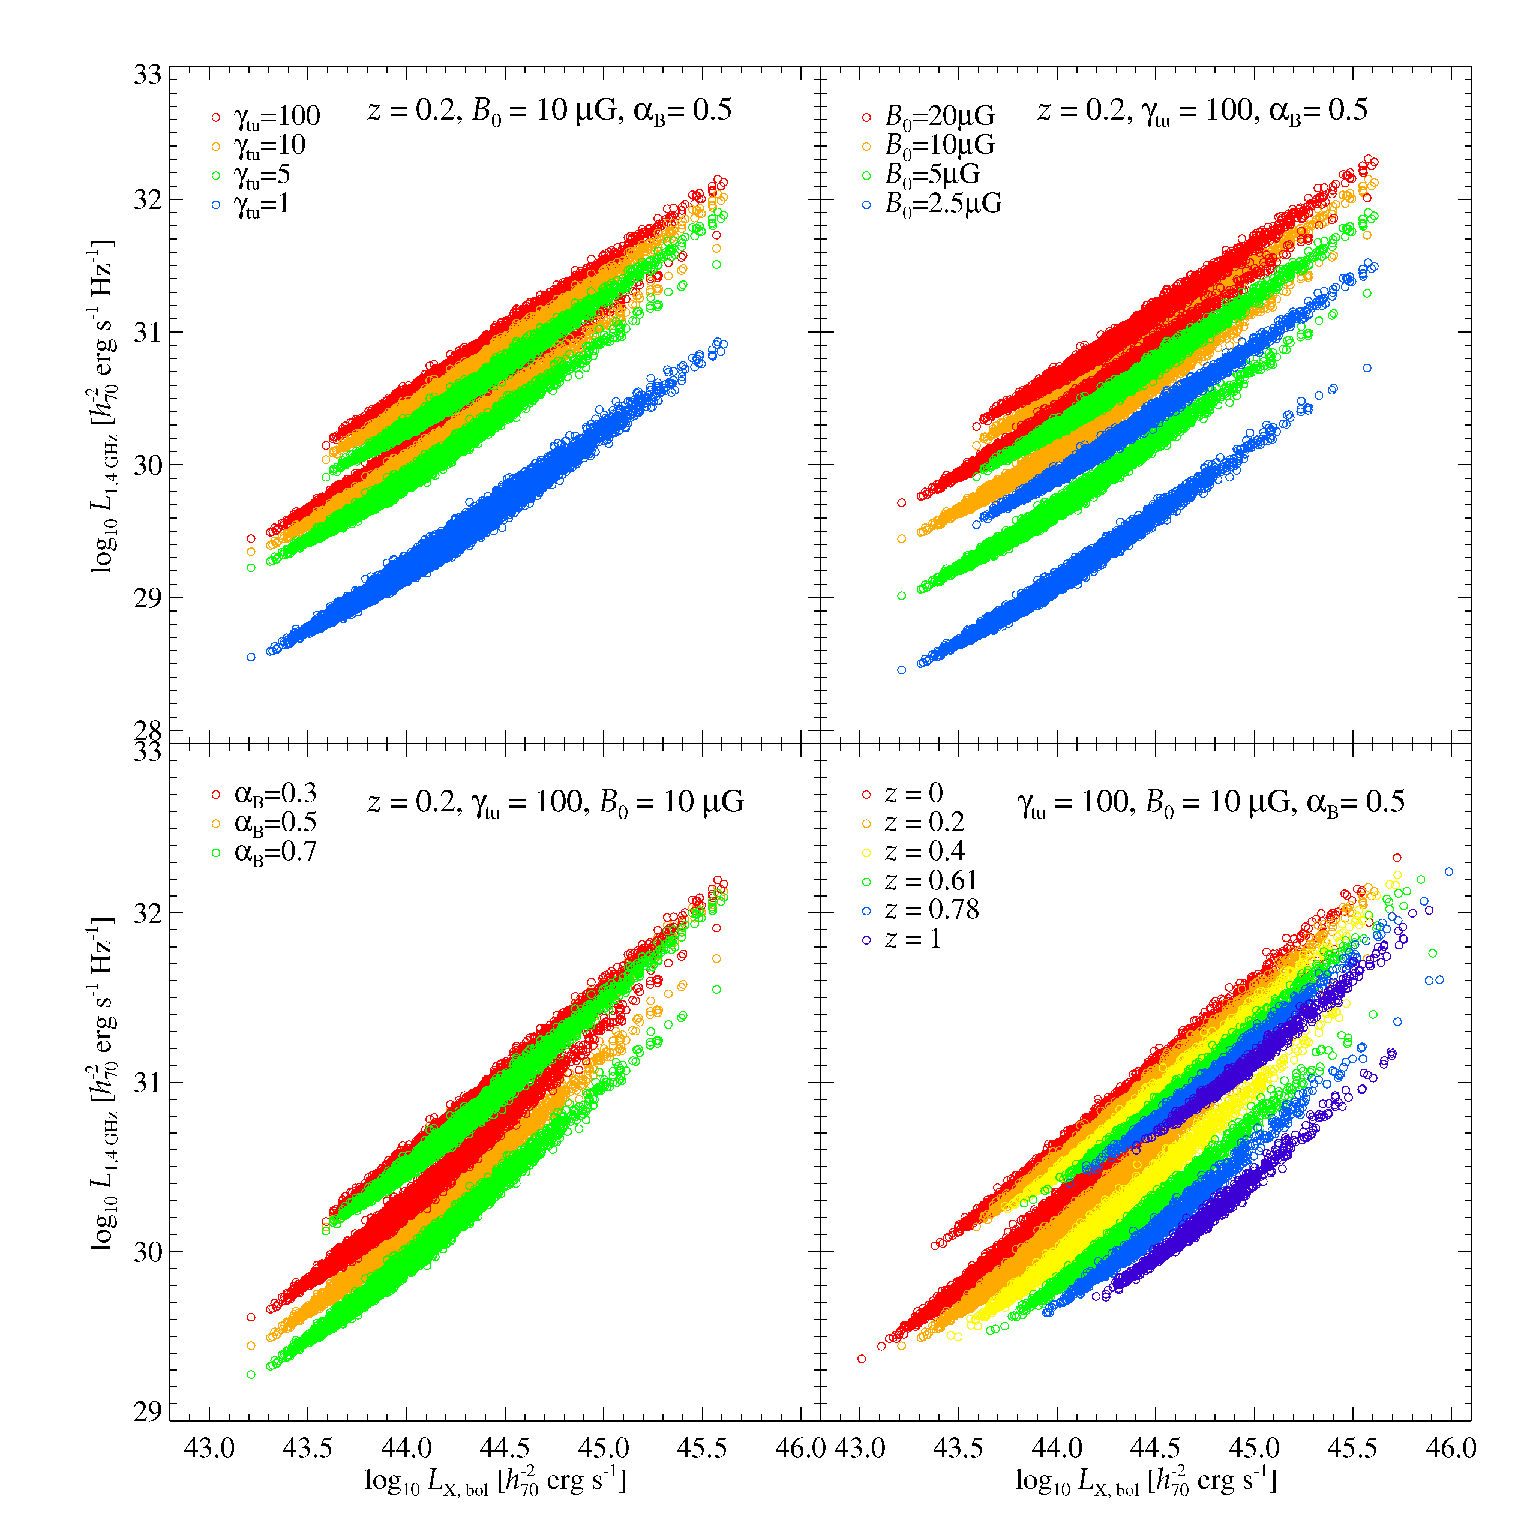
\includegraphics[width=0.49\textwidth]{figures/PL_relation_testing_gimp.eps}
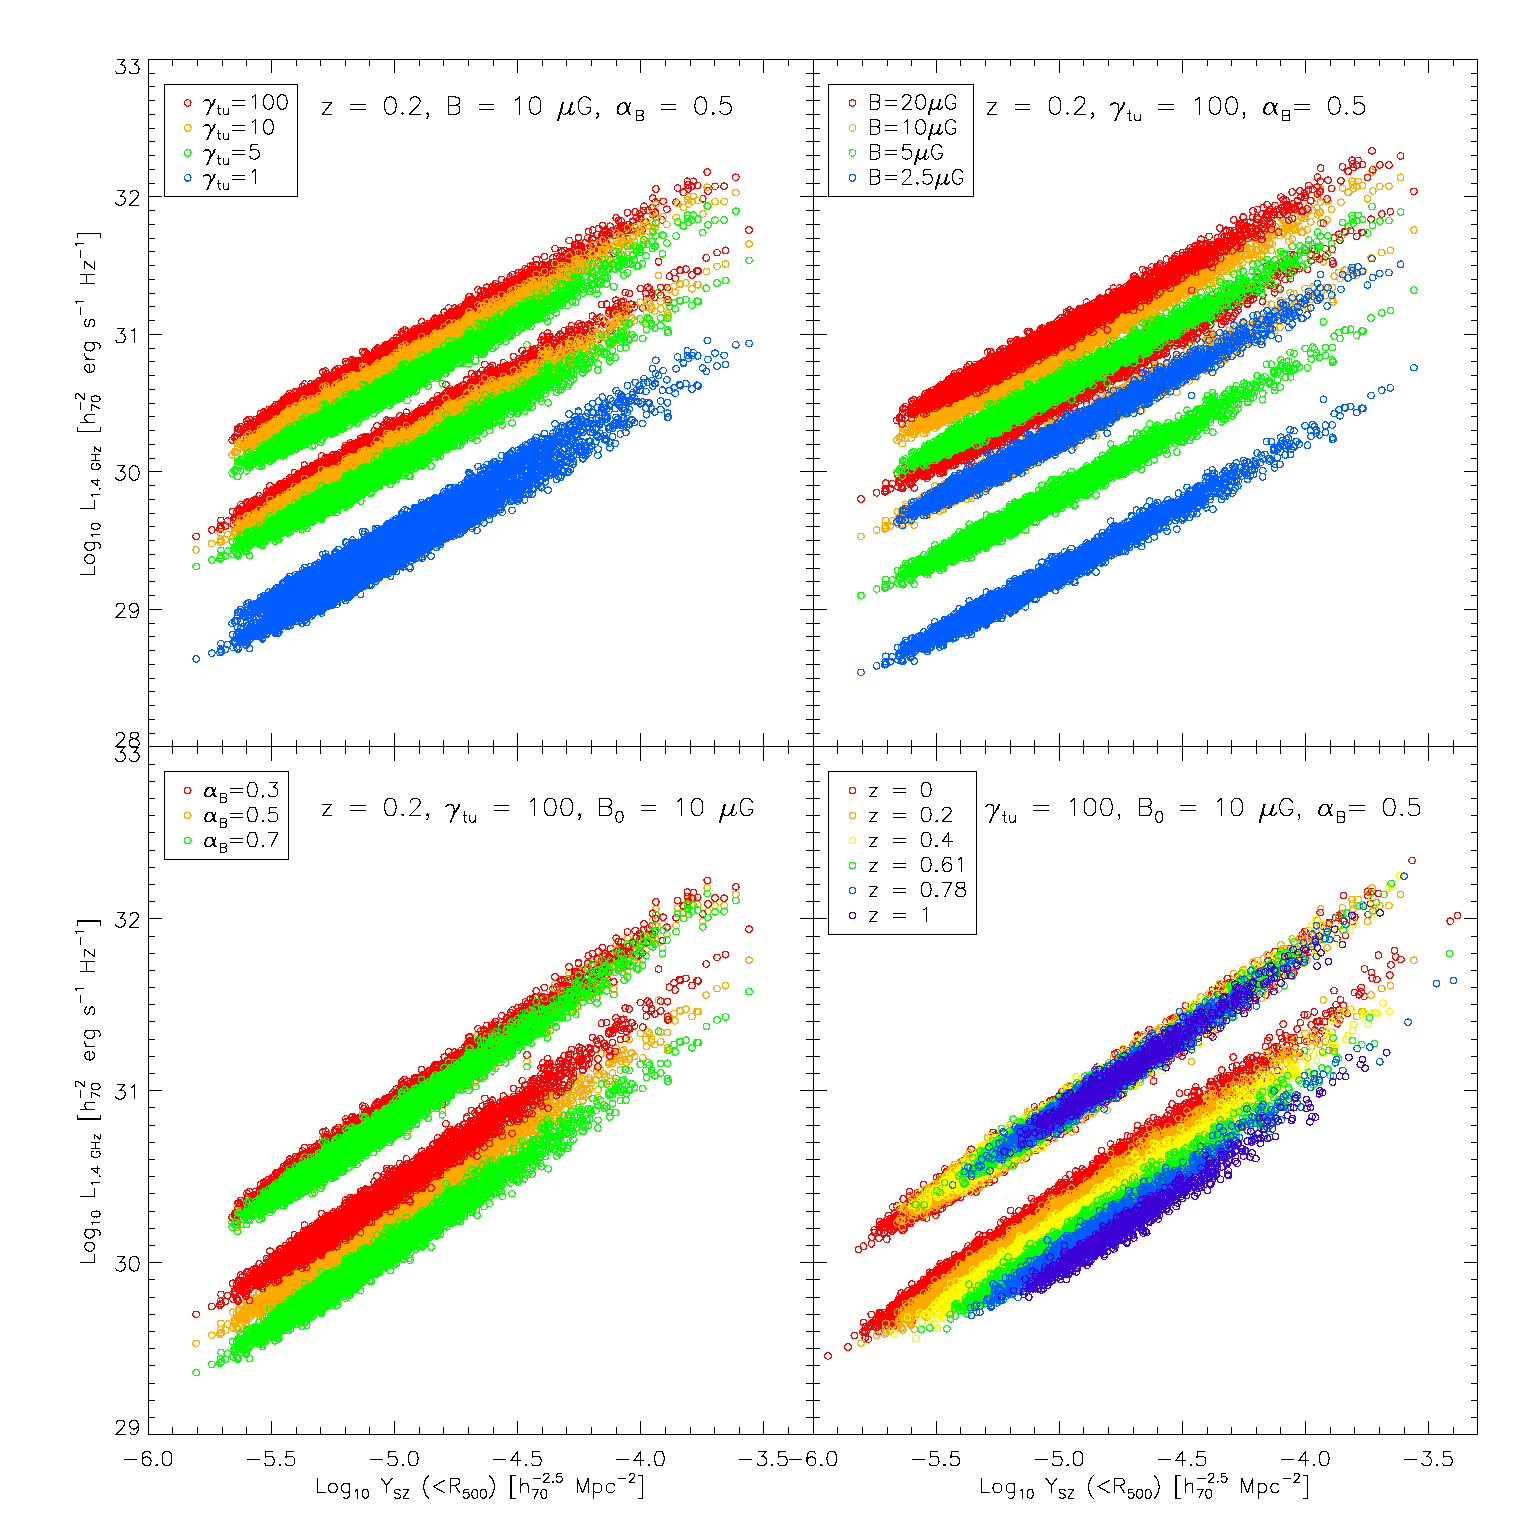
\includegraphics[width=0.49\textwidth]{figures/PSZ_relation_testing_gimp.eps}
\caption{Radio-to-X-ray and radio-to-SZ scaling relations as predicted by our
  extended CR model. In the left panel, we show how the
  $L_{1.4~\rmn{GHz}}-L_{\rmn{X,bol}}$ relation varies upon changing different
  parameters. In the right panel, we show the same, but for the
  $L_{1.4~\rmn{GHz}}-Y_{\rmn{SZ},500}$ relation. Note that in each plot there
  are two separated populations for each model realization, shown with the same
  color. The upper sets of points correspond to the CCC population while the
  lower sets correspond to NCCCs. The plot labels indicate those parameters
  which are kept fixed. We fix the $g_{\rmn{CR}}$-normalization parameter to 0.5
  for all cases. See main text for details.}
\label{fig:SR}
\end{figure*}


\section{Radio Scaling Relations}
\label{sec:4}
As introduced in Section~\ref{sec:1}, there exist an apparent bimodality between
the radio and X-ray cluster emission. Clusters with a given X-ray luminosity can
either host RHs or show an absence of diffuse radio emission (e.g.,
\citealp{2009A&A...507..661B,2011A&A...527A..99E}). More recently, a study of
the radio-to-SZ scaling relation revealed the absence of a strong bimodality
dividing the cluster population into radio-loud and radio-quiet clusters
\citep{2012MNRAS.421L.112B}. Since $Y_{\rmn{SZ}}$ correlates more tightly with
cluster mass than $L_{\rmn{X}}$, this may indicate that the larger scatter of
$L_{\rmn{X}}$ correlates with the scatter of the radio luminosity in such a way
that it produces a bimodality; but as a result of a second (hidden parameter)
rather than the fundamental cluster parameter---its mass. 

In this section, we investigate these two scaling relations in the framework of
our extended hadronic scenario. We refrain from modeling the leptonic emission
component, which we expect to be particularly important in radio-loud, high-mass
NCCCs because the dissipated energy that is available for energizing fossil
electrons should be a fraction of the thermal energy which scales with cluster
mass as $E_\rmn{th}\propto M_{200}^{5/3}$ \citep[][for magneto-turbulent
reacceleration models]{2005MNRAS.357.1313C}. For want of a better model, we
could boost the radio flux by some factor drawn from an ab initio unknown
distribution of leptonic luminosities. However, we refrain from such an approach
and defer the study of the physical details of this component and its
correlation to the hadronic component to future work. Additionally, the high-mass 
range where the leptonic emission component would have a decisive impact 
is affected by incompleteness of the simulation. Hence for a given set of
parameter choices, our radio halo fluxes are conservative lower limits; in
particular for the subsample of radio loud NCCCs.


\subsection{Exploring the parameter space of scaling relations}

In Fig.~\ref{fig:SR}, we show the general scaling relations of our extended CR
model of Section~\ref{sec:2.3} applied to the MultiDark sample. We show how both
the radio-to-X-ray and the radio-to-SZ scaling relations differ upon varying the
parameters $\gamma_{\rmn{tu}}$, $B_{0}$, $\alpha_{\rmn{B}}$ and redshift. We fix
the CR-normalization parameter $g_{\rmn{CR}}$ to 0.5 in all cases, ensuring an
average CR-to-thermal pressure of $2\%$ ($0.05\%$) within $R_{500}$
($R_{500}/2$). Here, the radio luminosity is calculated at $1.4$~GHz within
$R_{500}.$\footnote{The mean (median) difference between calculating $L_{\nu}$
  within $R_{200}$ or $R_{500}$ is 5.3\% (5.6\%).}  In our CR model, we fix the
CR number for $\gamma_{\rmn{tu}}=100$ using equation~(36) of
\cite{2011A&A...527A..99E}, integrating up to $R_{500}$. To compute the radio
luminosity for different values of $\gamma_{\rmn{tu}}$, we employ CR number
conservation (for CR energies $E>$~GeV where Coulomb cooling is negligible for CR
protons).

In each panel in Fig.~\ref{fig:SR} there are two separated populations for
each model realization (i.e., for a given set of parameters). Each upper set of
points corresponds to the CCC population while the lower set corresponds to
NCCCs, respectively. In our model, the radio and X-ray emissivities scale with
the square of the gas density so that $L_{1.4~\rmn{GHz}}$ and $L_{\rmn{X,bol}}$
are significantly higher for CCCs in comparison to NCCCs. In contrast,
$Y_{\rmn{SZ}}$ only depends weakly on the central gas density as explained in
Section~\ref{sec:X-SZ-scaling}. This explains the relative location of the NCCC and
CCC populations in the $L_{1.4~\rmn{GHz}}-L_{\rmn{X,bol}}$ and
$L_{1.4~\rmn{GHz}}-Y_{\rmn{SZ}}$ planes. In particular, CCCs are shifted to the
upper right in the $L_{1.4~\rmn{GHz}}-L_{\rmn{X,bol}}$ plane while they are
shifted vertically upward in the plane spanned by
$L_{1.4~\rmn{GHz}}-Y_{\rmn{SZ}}$. In reality, we expect an (ab initio unknown)
distribution of these parameters which would substantially increase the scatter
in the scaling relations and possibly lead to a bimodality, depending on
correlations among the different parameters.

Most interestingly, the slope of the radio scaling relations does not differ
when varying parameter values because we do not include any cluster
mass-dependence in our parametrizations which is neither required nor
constrained by current data. Closely inspecting Fig.~\ref{fig:SR}, we see that
we obtain the largest changes in $L_{1.4~\rmn{GHz}}$ for variations in
$1<\gamma_{\rmn{tu}}<5$ and $B_0$ over the parameter range probed, albeit with a
stronger dependence for weaker field strengths (as expected from
equation~(\ref{eq:jnu})).


\subsection{Comparison to observations}
\label{sec:scaling-obs}
 
After collecting the X-ray luminosity and the SZ flux of known RHs, we compare
the resulting scaling relations to a phenomenological model realization that was
chosen to additionally obey other observational constraints (e.g., from Faraday
rotation measure studies) as well as theoretical considerations on CR transport
presented in Section~\ref{sec:discussion_hadronic}.


\subsubsection{Observational samples}

In Appendix~\ref{app:D} we construct a sample of giant radio halos (black) and
radio mini-halos (red), as well as upper limits on the radio emission
\citep{2009A&A...499..371G,2009A&A...507..661B, 2011A&A...527A..99E}, and show
this in the left panel of Fig.~\ref{fig:PLSZ}. The median redshift of this
sample is $z\approx0.18$. The corresponding observational scaling relation is
well fit by $\log_{10} L_{1.4~\rmn{GHz}} = A + B~\log_{10} L_{\rmn{X,bol}}$ with
$A=-37.204\pm1.838$ and $B=1.512\pm0.041$, and a scatter of $\sigma_{yx} \approx
0.52$ (we do not include upper limits in the fit; units are as in
Fig.~\ref{fig:PLSZ}). We refer the reader to \cite{2009A&A...507..661B} and
\cite{2011A&A...527A..99E} for an extensive discussion on this topic. We
emphasize that in contrast to giant radio halos, mini-halos span a wider range
in radio luminosity (as also pointed out by \citealp{2009A&A...499..679M}). The
Perseus mini-halo (highest radio mini-halo luminosity in the left panel of
Fig.~\ref{fig:PLSZ}), e.g., has a radio luminosity that is almost an order of
magnitude higher than in giant radio halos at the same X-ray luminosity. In
contrast, the Ophiuchus mini-halo (lowest radio mini-halo luminosity in the left
panel of Fig.~\ref{fig:PLSZ}), which is representative of a few other similar
examples recently detected in CCCs (such as A2029 and A1835), has a radio
luminosity which is much lower than giant radio halos in merging clusters and is
even below the upper limits.

We caution that the determination of the slope of the observational
$L_{1.4}-L_{\rmn{X,bol}}$ relation is not very robust because of the small
sample size of RHs, selection biases of extended low-surface brightness objects,
and systematic uncertainties in the measurements of $L_{1.4}$ and
$L_{\rmn{X,bol}}$. The recently detected low-luminosity mini-halos exemplify
those uncertainties and the large intrinsic scatter of this relation. On the
other hand, X-ray luminosities for the same object as derived by,
e.g.,~\emph{ROSAT} and \emph{Chandra} can easily differ by a factor of a
few.\footnote{For example, the bolometric X-ray luminosity of A2163 as measured
  by \emph{ROSAT} is $8.65\times10^{45}$~$h_{70}^{-1}$~erg~s$^{-1}$
  \citep{2009A&A...507..661B} while the \emph{Chandra} measurement is
  $4.93\times10^{45}$~$h_{70}^{-1}$~erg~s$^{-1}$ (\citealp{2009ApJS..182...12C};
  ACCEPT: Archive of Chandra Cluster Entropy Profile Tables;
  http://www.pa.msu.edu/astro/MC2/accept/).}  In the left panel of
Fig.~\ref{fig:PLSZ}, we additionally show the model of
\citet{2009JCAP...09..024K} with a slope of $\approx1.2$, arbitrarily normalized
for visual purposes, from their simple analytical hadronic model.

In order to compare our model to the observed 1.4~GHz radio-to-SZ scaling
relation, we use the result by \cite{2012MNRAS.421L.112B} that is based on the
radio halo sample from \cite{2007MNRAS.378.1565C} (hereafter C07), which has a
median redshift of $z \approx 0.18$ and excludes radio mini-halos. For this
sample, \cite{2012MNRAS.421L.112B} computes $Y_{\rmn{SZ}}$ within the radio-halo
radii given by \cite{2007MNRAS.378.1565C}. These radii have a median of about
$0.5$~$h_{70}^{-1}$~Mpc which compares favourably with the median of $R_{500}
\approx 0.4$~$h_{70}^{-1}$~Mpc in our MultiDark $z = 0.2$ snapshot. For the C07
sample, \cite{2012MNRAS.421L.112B} obtains a scaling relation in the form of
$\log_{10} L_{1.4~\rmn{GHz}} = A + B~\log_{10} Y_{\rmn{SZ}}$ with $A=29.7\pm0.8$
and $B=1.17\pm0.18$, and a scatter of $\sigma_{yx} \approx 0.28$ (units are as
in Fig.~\ref{fig:PLSZ}). The same comments regarding the small sample size of
RHs, selection biases, and systematic uncertainties in the luminosity
measurements also apply here.


\subsubsection{Model realization}

\begin{figure*} 
\centering
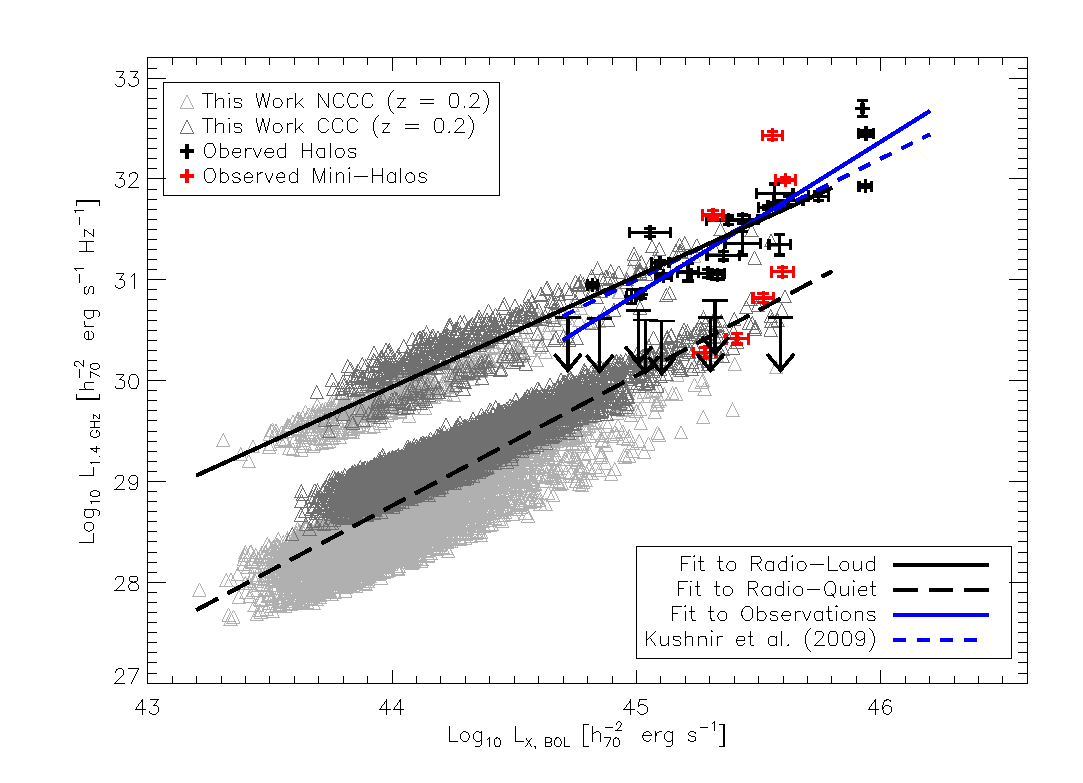
\includegraphics[width=0.49\textwidth]{figures/PL_relation.eps}
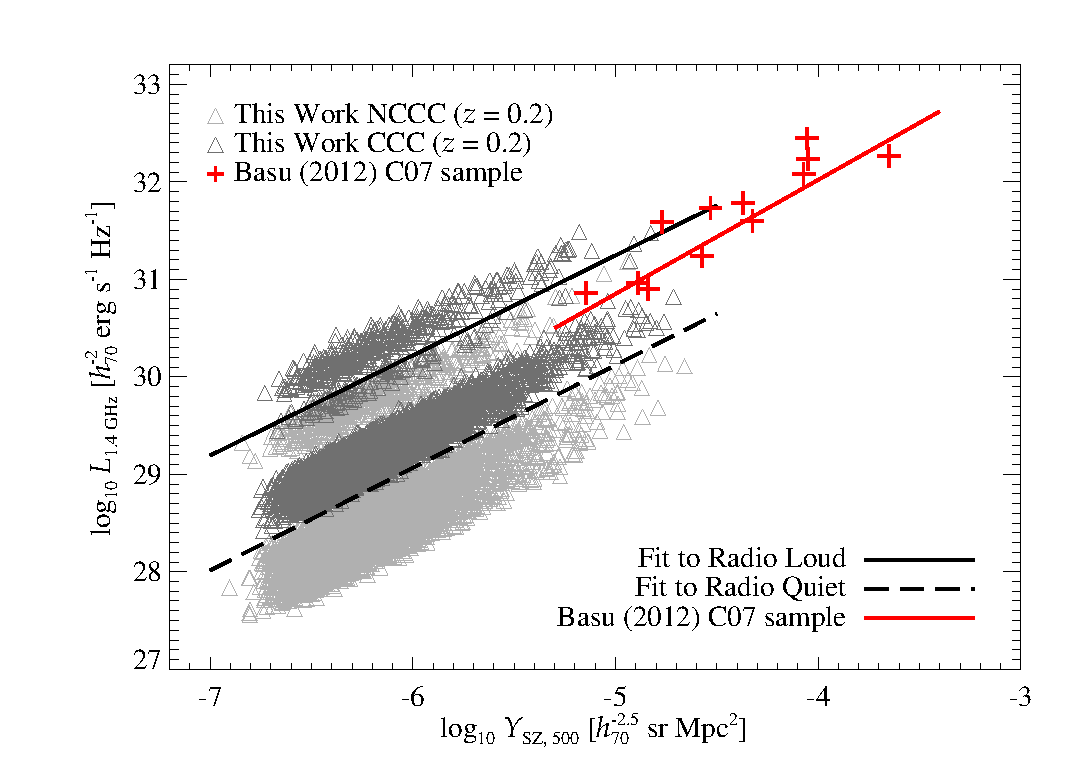
\includegraphics[width=0.49\textwidth]{figures/PSZ_relation.eps}
\caption{Radio-to-X-ray and radio-to-SZ scaling relations in our extended CR model
  (see main text for the details of the chosen parameters) compared with
  observations.  \emph{Left.} $L_{1.4~\rmn{GHz}}-L_{\rmn{X,bol}}$ relation in
  comparison to the observational sample taken from the literature and detailed
  in Appendix~\ref{app:D}. \emph{Right.} $L_{1.4~\rmn{GHz}}-Y_{\rmn{SZ}}$
  relation in comparison to the observational sample C07 from
  \protect\cite{2012MNRAS.421L.112B}.}
\label{fig:PLSZ}
\end{figure*} 

In order to compare our model prediction with observations, we select a
particular realization of our model. To this end, we use the MultiDark cluster
sample at $z=0.2$, which compares well with the redshift of the observational
samples; see above and Appendix~\ref{app:D}. We divide our cluster sample
randomly into radio-quiet and radio-loud clusters, assuming a ratio of $10\%$ of
the latter. We use the turbulent propagation parameter $\gamma_{\rmn{tu}}$ to
separate both populations. In radio-quiet clusters, we assign
$\gamma_{\rmn{tu}}=1$, and in radio-loud clusters, we adopt randomly and
uniformly $\gamma_{\rmn{tu}}$ values in the intervals $[40,80]$ and $[1,5]$ for
NCCCs and CCCs, respectively. As eluded before, we only model the hadronic
emission component and neglect the possible leptonic component which could
result in an under-prediction of radio halo fluxes of radio loud NCCCs.

Our modeling of magnetic fields is inspired by Faraday rotation studies that
point to higher field values in the core region of CCCs compared to NCCCs
\citep{2011A&A...529A..13K, 2010A&A...513A..30B}, presumably due to the higher
adiabatic compression factor during the formation of the cooling core. Hence,
for radio-quiet clusters, we adopt randomly and uniformly distributed values of
the central magnetic field $B_0$ in the intervals $[2.5,5.5]$~$\mu$G and
$[5,10]$~$\mu$G for NCCCs and CCCs, respectively. To account for the potential
turbulent dynamo in radio-loud objects (characterized by a higher turbulent
transport parameter in our model), we slightly increase $B_0$ in those objects
and chose $B_0$ intervals of $[4.5,7.5]$~$\mu$G and $[7.5,12.5]$~$\mu$G for
NCCCs and CCCs, respectively.

We fix $\alpha_{\rmn{B}}=0.5$ and $g_{\rmn{CR}}=0.5$ for all clusters. We note
that our parameter choices are mostly phenomenologically driven with the aim to
reproduce observations. The parameter study in Fig.~\ref{fig:SR} exemplifies
considerable degeneracies so that different combinations of parameters can
potentially result in very similar distributions. We emphasize the need of more
detailed observations of radio halos and in particular of multi-frequency
correlation studies to constrain the interplay of some of these parameters.

In Fig.~\ref{fig:PLSZ}, we show our model in comparison to the observed
radio-to-X-ray and radio-to-SZ scaling relations. The normalization of our model
can be arbitrarily varied by changing $g_{\rmn{CR}}$ as long as the resulting
$X_{\rmn{CR}}$ respects the current observational constraints
(e.g., \citealp{2011arXiv1111.5544M}) and remains below a few percents. As
explained above, our choice of $g_{CR}=0.5$ ensures an average CR-to-thermal
pressure of $2\%$ within $R_{500}$, allowing for plenty of available parameter
space to match the observational constraints.  Our model is sufficiently
flexible to either mimic a cluster radio bimodality or not, depending on the
parameters adopted for the populations of radio-loud and radio-quiet
objects. 

However, with the given model realization as in Fig.~\ref{fig:PLSZ}, the
separation of the radio-loud and radio-quiet populations is substantially larger in
the $L_{1.4~\rmn{GHz}}-L_{\rmn{X,bol}}$ plane than in the
$L_{1.4~\rmn{GHz}}-Y_{\rmn{SZ}}$ plane, which exhibits almost a continuum
distribution from radio-loud CCCs to the radio-quiet NCCCs. This is mainly
because the bolometric X-ray emissivity scales with $\rho_{\rmn{gas}}^2$ while
$Y_{\rmn{SZ}}\propto\rho_{\rmn{gas}}$ (which is only strictly valid for an
isothermal gas distribution). As a consequence, the highly peaked gas profiles
of CCCs have less impact on $Y_{\rmn{SZ}}$ than on $L_{\rmn{X,bol}}$. This is
one plausible explanation for the observed discrepancy of the presence of a
bimodality in $L_{1.4~\rmn{GHz}}-L_{\rmn{X,bol}}$ and the apparent absence of it
in $L_{1.4~\rmn{GHz}}-Y_{\rmn{SZ}}$. 

The slope of our model depends on the different parameter choices and,
particularly, on the relative differences introduced for the NCCC/CCC and the
radio-loud/quiet populations. However, we note that our
$L_{1.4~\rmn{GHz}}-L_{\rmn{X,bol}}$ is slightly shallower than the observed
relation, more similar to the \cite{2009JCAP...09..024K} prediction.
Potentially this may hint at the contribution of a second, leptonic component
that would steepen the slope of our model scaling relation and which we
neglected here for simplicity. In contrast, the slope of our
$L_{1.4~\rmn{GHz}}-Y_{\rmn{SZ}}$ compares well with the observed slope. Owing to
the many uncertainties and lack of robustness both in the observations and
modeling at this stage, we do not attempt to fine-tune our model to the
observations.



%%%%%%%%%%%%%%%%%%%%%%%%%%%%%%%%%%%%%%%%%%%%%%%%%%%%%%%%%%%%%%%%%%%
%%%%%%%%%%%%%%%%%%%%%%%%%%%%%%%%%%%%%%%%%%%%%%%%%%%%%%%%%%%%%%%%%%%
\section{Radio Luminosity Function}
\label{sec:5}

\begin{figure*} 
\centering
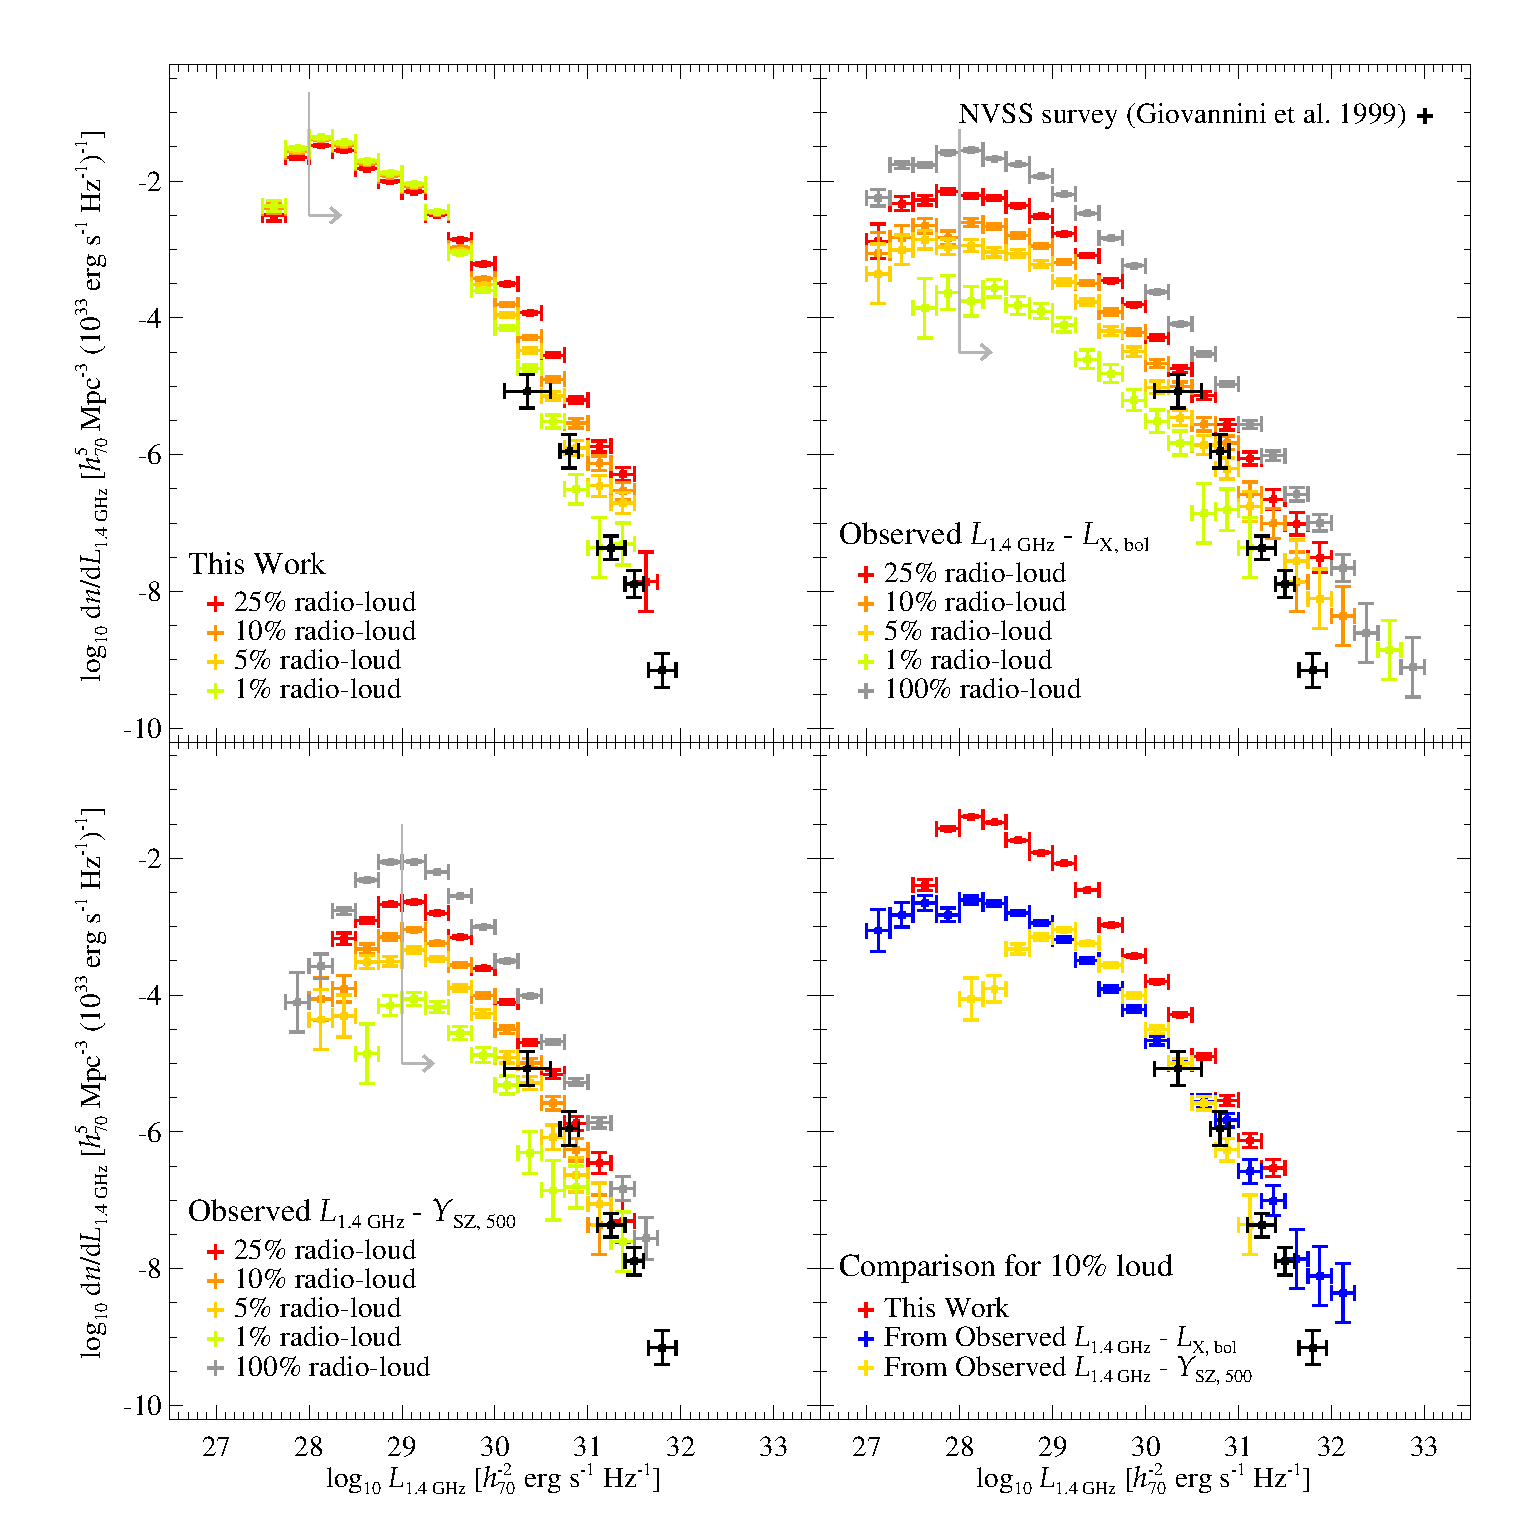
\includegraphics[width=0.85\textwidth]{figures/RLFs_1.4.eps}
\caption{RH luminosity function (RLF) at 1.4~GHz. The top left panel shows
  the RLF of our extended CR model (see main text for the details of the chosen
  parameters) for different fractions of radio-loud clusters. Additionally shown
  is the contribution of radio-quiet and radio-loud populations to the total RLF
  (assuming a fraction of $25\%$ and $1\%$ of radio-loud objects). The top right
  panel shows the RLF obtained by applying the observed
  $L_{1.4~\rmn{GHz}}-L_{\rmn{X,bol}}$ relation to the MultiDark clusters at $z =
  0.2$, using our phenomenological gas model for $L_{\rmn{X,bol}}$ of each
  cluster; again for different percentages of radio-loud clusters.  The bottom
  left panel shows the RLF obtained by applying the observed
  $L_{1.4~\rmn{GHz}}-Y_{\rmn{SZ}, 500}$ relation to the MultiDark clusters at $z
  = 0.2$, using $Y_{\rmn{SZ}, 500}$ of our our phenomenological gas model
  for each cluster. The bottom right panel shows the comparison between the
  three approaches for 10\% of radio-loud clusters. In all panels, we show the
  NVSS survey RLF \citep{1999NewA....4..141G} with a median redshift of 
  $z\approx 0.18$, corrected for the sample incompleteness and survey sky coverage. 
  Horizontal error bars represent the mass bins while the vertical error bars are Poissonian 
  uncertainties. The light gray line marked by the arrow estimates the incompleteness limit owing
  to the adopted low-mass cut (Section~\ref{sec:2}) and the scatter in the
  halo luminosities.}
\label{fig:RLF_1.4}
\end{figure*}


\subsection{Comparison with observations at 1.4~GHz}

In Fig.~\ref{fig:RLF_1.4}, we show the RH luminosity function (RLF) at 1.4~GHz
for a representative realization of our extended CR model (as in
Section~\ref{sec:4}), and compare it with observational results. As for the XLF,
the RLF is completely determined by the cluster mass function and the radio
luminosity-to-mass relation, through $L_{1.4~\rmn{GHz}}-L_{ \rmn{X,bol}}$ or
$L_{1.4~\rmn{GHz}}-Y_{\rmn{SZ}}$ in combination with our phenomenological gas
model. However, in the radio band there is the additional uncertainty of the
fraction of radio-loud clusters. Thus, in Fig.~\ref{fig:RLF_1.4}, we also show
the RLFs obtained by applying the $L_{1.4~\rmn{GHz}}-L_{\rmn{X,bol}}$ and
$L_{1.4~\rmn{GHz}}-Y_{\rmn{SZ}}$ relations to simulated clusters of the
MultiDark snapshot at $z = 0.2$, using our phenomenological gas model for
$L_{\rmn{X,bol}}$ and $Y_{\rmn{SZ}, 500}$ of each cluster, respectively. Note
that this procedure is {\em only} applied to halos defined as radio-loud
clusters (which are by definition accounted for in the $L_{1.4~\rmn{GHz}}$
scaling relations) and we assume a fraction of 100\%, 25\%, 10\%, 5\% and 1\% of
radio-loud clusters. As evident from Fig.~\ref{fig:RLF_1.4}, this is different
from our model for the radio luminosity, where we also define a fraction of
radio-loud clusters. However, the radio-quiet population also contributes to the
RLF with an increasing fraction at low luminosities. This is exemplified in the
top left plot of Fig.~\ref{fig:RLF_1.4}, which shows the contribution of
radio-quiet and loud populations to the total RLF, assuming a fraction of $25\%$
and $1\%$ of radio-loud objects.

In Appendix~\ref{app:D}, we make an attempt to construct an RLF from existing
X-ray flux-limited radio surveys. There exist two such studies, the cluster
radio survey done with the National Radio Astronomy Observatory (NRAO) Very
Large Array (VLA) sky survey (NVSS) at $1.4$~GHz of \cite{1999NewA....4..141G}
and the survey with the Giant Metrewave Radio Telescope (GMRT) at $610$~MHz by
\cite{VenturiGMRT_1,VenturiGMRT_2}. For the latter, one can also construct an RLF
at 1.4~GHz using the corresponding RH follow-up measurements. The fractions of
radio-loud clusters are about 6\%, 18\% and 24\% for the NVSS 1.4~GHz, GMRT
610~MHz and GMRT 1.4~GHz samples, respectively. As explained in
Appendix~\ref{app:D}, we use the 1.4~GHz NVSS RLF (with a median redshift of $z
\approx 0.18$) as observational reference for our comparisons. We conclude that
the observational determinations of the RLF is not very robust at this stage;
the very different fractions of radio-loud clusters found in the different
studies is one indicator of this.
  
Generally, there is fair agreement between the NVSS RLF and both our modeled RLF
and the RLFs based on observational scaling relations, particularly for
radio-loud fractions between 10\% and 1\%. In particular, we verified that the
cumulative number of RHs above a certain flux limit of the NVSS survey is well
matched by our 10\%-loud fraction case, which will be used in the following
section.  The RLF obtained from the $L_{1.4~\rmn{GHz}}-L_{\rmn{X,bol}}$ relation
differs from the NVSS RLF at high luminosities, presumably caused by the large
observed scatter.  On the other side, the RLF obtained from the
$L_{1.4~\rmn{GHz}}-Y_{\rmn{SZ}}$ relation matches the NVSS result better. These
results need to be consolidated by RLFs corrected for flux-incompleteness and
simulations of larger cosmological volumes that are more complete at the
high-mass end. Figure~\ref{fig:RLF_1.4} shows that it will be difficult to
discriminate between different scenarios at high radio luminosities (or
equivalently masses). Indeed, in the bottom right panel of
Fig.~\ref{fig:RLF_1.4} we compare our RLF and the RLFs based on observational
scaling relations for a 10\% fraction of radio-loud clusters to the NVSS
RLF. This suggests that the low-luminosity (low-mass) clusters will be the most
useful in disentangling between different models. This emphasizes the importance
of conducting homogeneous, well controlled surveys of radio halos with the
Jansky VLA, ASKAP \citep{2011PASA...28..215N} and APERTIF
\citep{2012JApA..tmp...34R} at 1.4 GHz and LOFAR at lower frequencies. Since the
latter has already started to take data, it is extremely timely to present RLF
predictions for this wavelength regime in our model, which we will do next.


\subsection{Low-frequency predictions at 120~MHz}

In Fig.~\ref{fig:RLF_120}, we show our model predictions at 120~MHz obtained
with the same representative realization of our model as in Section~\ref{sec:4},
with 10\% radio-loud clusters. We show both the differential RLF (top left
panel) and the cumulative number density (bottom left panel) at different
redshifts (corresponding to different MultiDark snapshots of Table~1).  We note
that the redshift evolution is almost entirely due to the
$1/(\epsilon_{\rmn{B}}+\epsilon_{\rmn{CMB}})$ factor of equation~(\ref{eq:jnu})
since $\epsilon_\rmn{CMB}\propto (1+z)^4$.  Our imposed mass cutoff of
$M_{200}=10^{14}\,h^{-1}\,M_\odot$, which has been adopted to reliably model the
cluster gas distribution, translates into a luminosity cutoff. This causes the
differential luminosity function to turn over at the low-luminosity end and may
artificially flatten the slope already at sightly higher luminosities than the
luminosity maximum that indicates our formal incompleteness limit.  Note that
calibrating our model to 1.4~GHz observations may cause an overestimate of the
number of low-frequency halos since we are neither considering any spectral
steepening due to CR transport nor a variation of the fractional hadronic
contribution to the radio-loud NCCC population with decreasing frequencies.

\begin{figure*} 
\centering
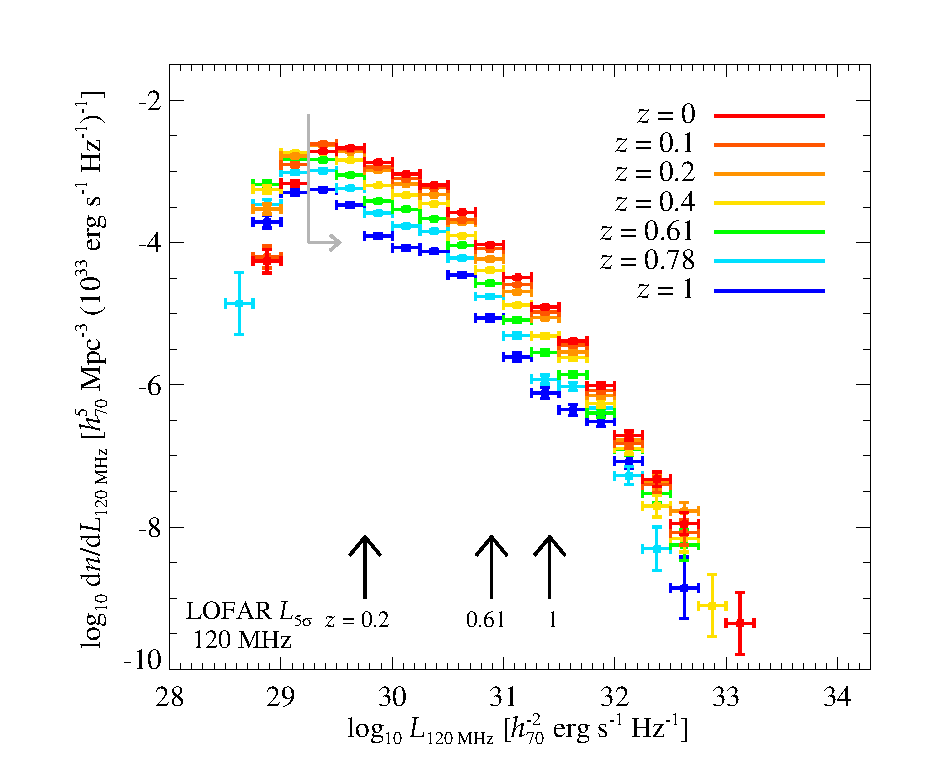
\includegraphics[width=0.5\textwidth,height=0.305\textheight]{figures/RLF_LOFAR.eps}
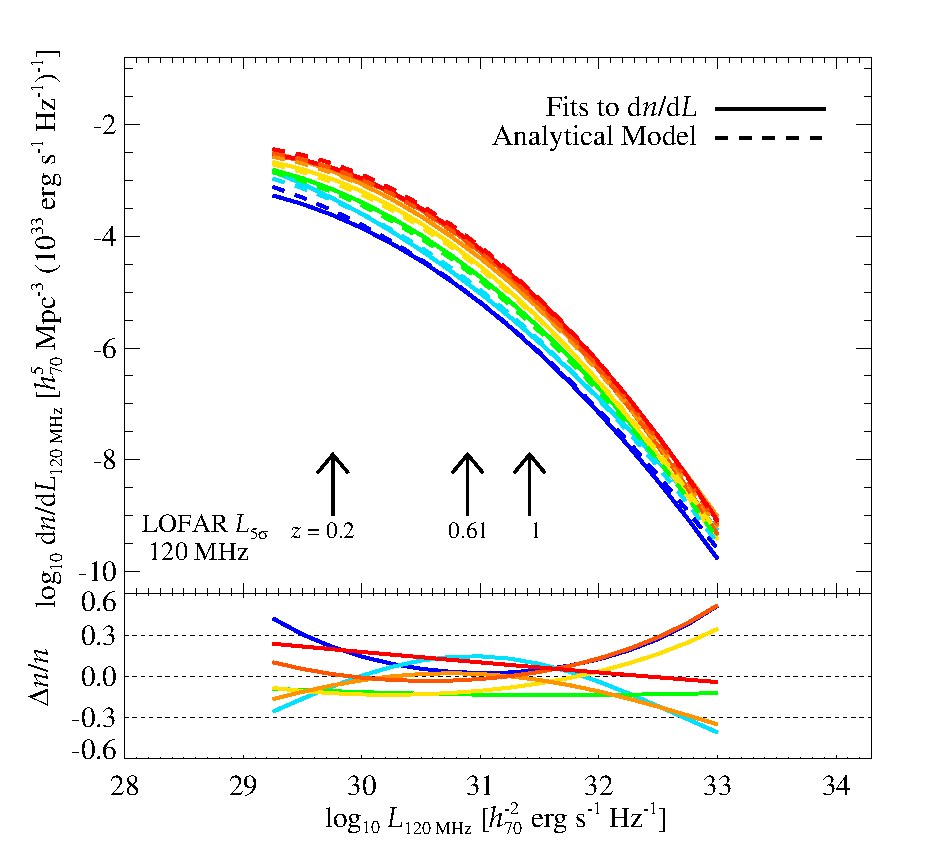
\includegraphics[width=0.47\textwidth,height=0.3\textheight]{figures/RLF_LOFAR_analytical_1.eps}
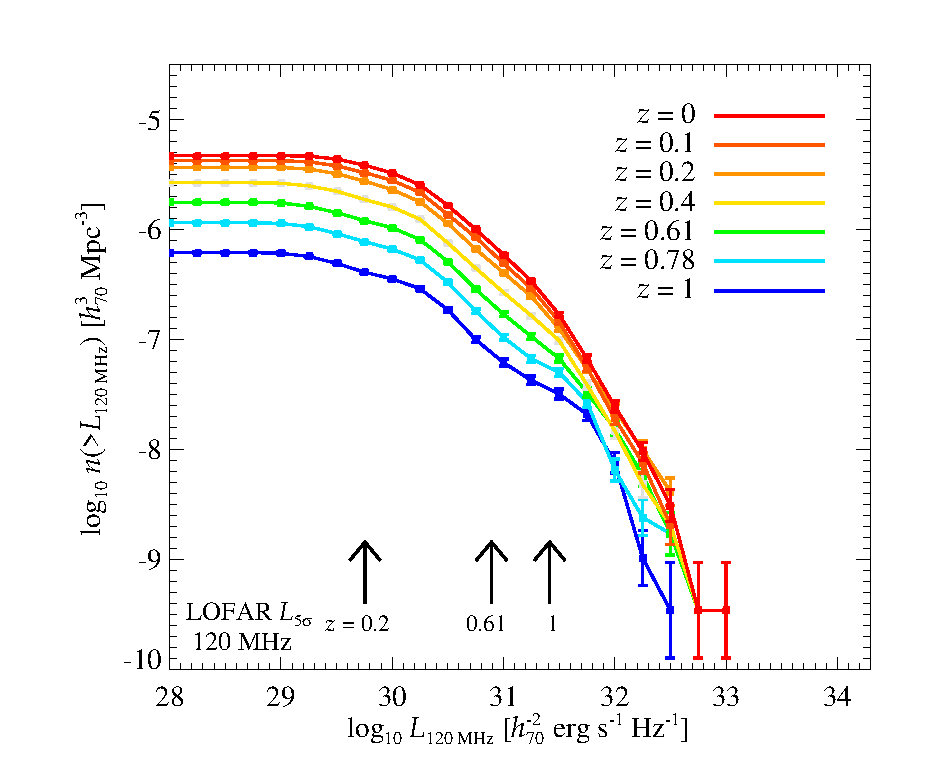
\includegraphics[width=0.5\textwidth,height=0.305\textheight]{figures/CumDensityL_LOFAR.eps}
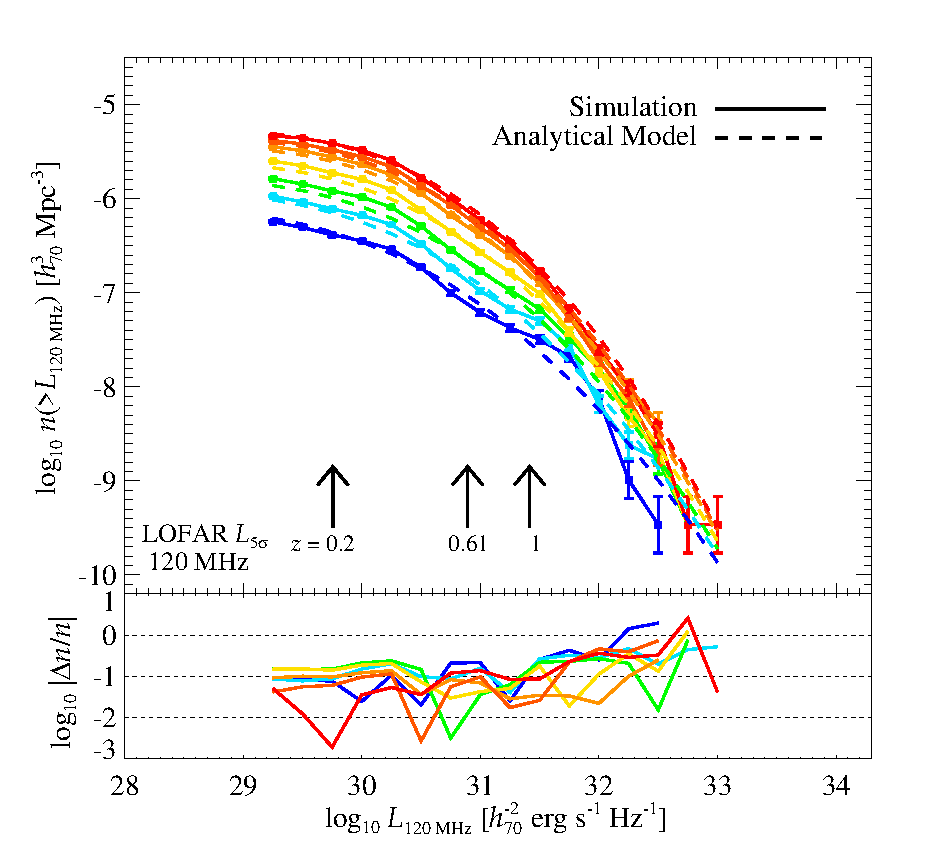
\includegraphics[width=0.47\textwidth,height=0.3\textheight]{figures/CumDensityL_LOFAR_1.eps}
\caption{RH luminosity function $n(L,z)$ at 120~MHz (top left panel) and cumulative
  number density of RHs  $n(>L,z)$ (bottom left panel) at different redshifts $z$ (color
  coded) for the model realization described in Section~\ref{sec:4} with a 10\%
  fraction of radio-loud clusters. To obtain an analytical model for $n(L,z)$,
  we fit the logarithm of the RLF at each $z$ with a second-order polynomial and
  constrain the evolution of the three free parameters to follow a linear
  function in $1+z$ (see main text for details). The right panels show the
  comparison of the RLF fits (top) and the cumulative number density of the
  MultiDark samples (bottom) to the constrained analytical model. The bottom panels of these
  two panels show the relative differences $\Delta n / n =
  (n_{\rmn{analytical}} - n_{\rmn{fit}})/n_{\rmn{fit}}$. Additionally shown is
  the LOFAR Tier~1 \emph{point-source} flux limit of
  $F_{5\sigma}^{\rmn{PS}}=0.5$~mJy \citep{2012JApA..tmp...34R} converted to a
  luminosity limit at a given redshift. Horizontal error bars represent the mass
  bins while the vertical error bars are Poissonian uncertainties.  The light
  gray line marked by the arrow estimates the incompleteness limit owing to the
  adopted low-mass cut (Section~\ref{sec:2}) and the scatter in the halo
  luminosities.}
\label{fig:RLF_120}
\end{figure*} 

Additionally shown in Fig.~\ref{fig:RLF_120} is the expected LOFAR Tier~1
\emph{point-source} flux limit of $F_{5\sigma}^{\rmn{PS}}=0.5$~mJy
\citep{2012JApA..tmp...34R} converted to a luminosity limit at a few representative
redshifts. This flux limit is clearly an underestimate for nearby RHs, which
extend over angular scales $\sim1$~deg, as e.g., in the case of the Coma radio
halo. In order to make more reliable predictions, in the following, we will
calculate the RH flux limit with equation~(10) of \cite{2010A&A...509A..68C},
approximating the halo extension by $R_{500}$ and requiring the mean flux within
the RH half-radius to be higher than $F_{5\sigma}^{\rmn{PS}}$. This may result
in an overestimation of the flux limit for CCCs, whose radio emission is more
centrally concentrated than in NCCCs. The median $R_{500}$ of our sample is
about $0.4$~$h_{70}^{-1}$~Mpc at all redshifts. This translates to a flux limit
of about $30$~mJy at $z = 0.1$, $7$~mJy at $z = 0.2$ and $0.5$~mJy (equal to the
point-source value) at $z \approx 0.6$.

\begin{figure*} 
\centering
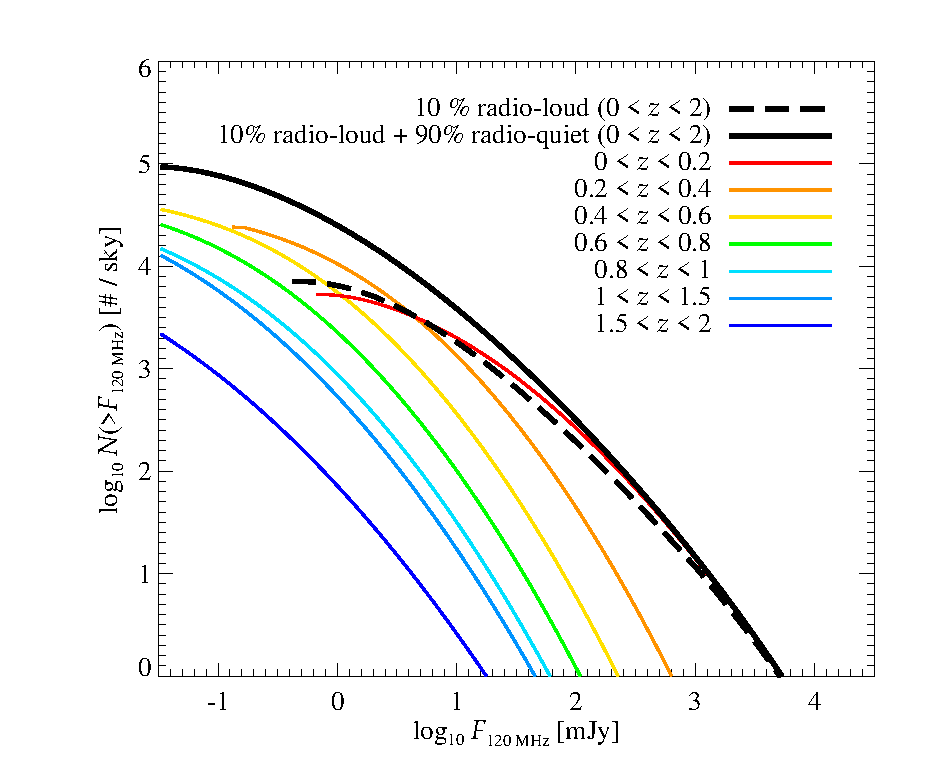
\includegraphics[width=0.48\textwidth]{figures/RLF_LOFAR_flux.eps}
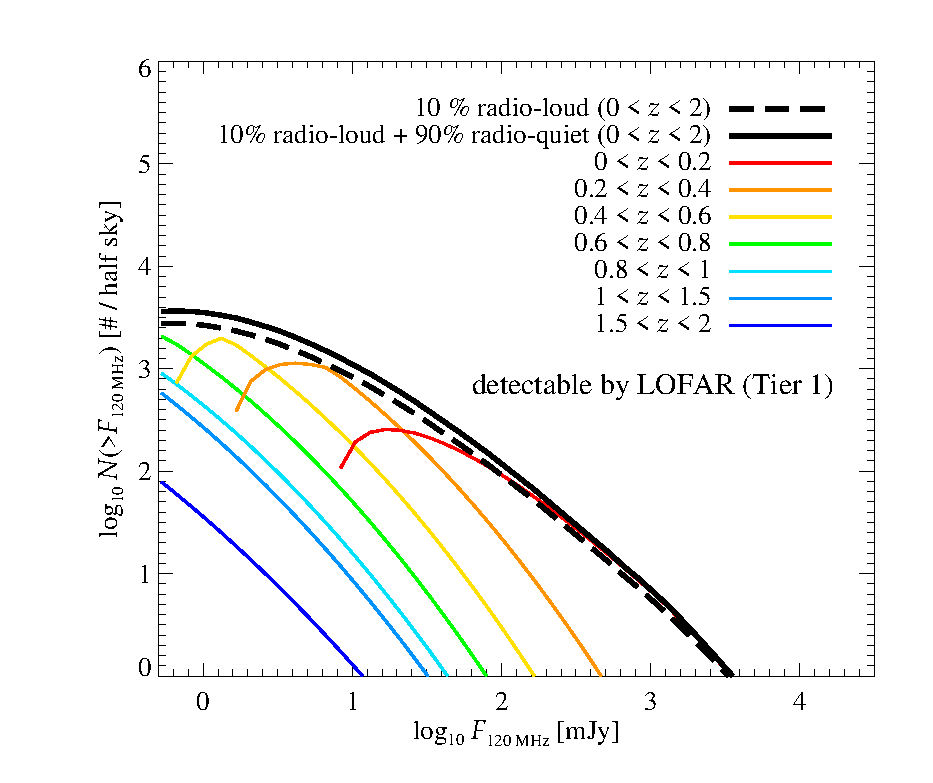
\includegraphics[width=0.48\textwidth]{figures/RLF_LOFAR_flux_detectable.eps}
\caption{Cumulative number of RHs above a certain flux limit in an all-sky
  survey at 120~MHz. We show the result of the model realization described in
  Section~\ref{sec:4} using all clusters and adopting a fraction of 10\% of
  radio-loud clusters (black solid line). Additionally, we show the result
  obtained by using the 10\% radio-loud clusters \emph{only} (black dashed
  line). We also show the differential contribution to the RLF in redshift
  slices. Note that the number of (detectable) RHs would be dramatically reduced
  by the presence of a break in the model at some low luminosity-scale, or a
  mass-dependence of the model parameters causing the RH luminosities to
  decrease at low masses.  \emph{Left.} Total number of RHs in the sky.
  \emph{Right.} Number of detectable RHs by the LOFAR Tier~1 survey considering
  its sky coverage (half sky) and adopting a realistic flux limit corresponding
  to different angular source extensions at different redshifts. The
  point-source flux limit, which applies to distant clusters with $z\gtrsim0.6$,
  is taken to be $F_{5\sigma}^{\rmn{PS}}=0.5$~mJy (see main text for details).
}
\label{fig:RLF_120_flux}
\end{figure*}

To derive low-frequency flux functions, we construct an analytical model for the
evolving RLF. We fit the 120~MHz RLF at different redshifts with a second-order
polynomial of the form $\log_{10} \rmn{d}n/\rmn{d}L_{120~\rmn{MHz}} = A_{0} +
A_{1}~\log_{10} L_{120~\rmn{MHz}} + A_{2}~(\log_{10} L_{120~\rmn{MHz}})^{2}$.
All luminosities are measured in units of $h_{70}^{-2}
\rmn{erg~s}^{-1}\,\rmn{Hz}^{-1}$ and (comoving) number densities in units of
$h_{70}^{3}\,\rmn{Mpc}^{-3}$. We consider only luminosities with $\log_{10}
L_{120~\rmn{MHz}} \geq 29.25$ to exclude the turn-over at low luminosities
caused by incompleteness. To obtain an analytical model for $n(L,z)$, we
constrain the evolution of the three free parameters $A_i$ to follow a linear
function in $1+z$, i.e., $A_{i} = A_{i,0} + A_{i,1}~(1+z)$.\footnote{The values
  of these parameters are $A_{0,0} = -436.79$, $A_{0,1} = 109.75$, $A_{1,0} =
  29.68$, $A_{1,1} = -7.17$, $A_{2,0} = -0.51$ and $A_{2,1}$ = 0.12.} In the
right panels of Fig.~\ref{fig:RLF_120}, we compare the RLF fits (top) and the
cumulative number density in the simulation (bottom) to the analytical model. In
particular the analytics matches the simulation well except for high
luminosities and high redshifts where small number statistics explains the
deviations.

This analytical model describes the number of RHs expected in our model per unit
luminosity and per unit comoving volume $V_{\rmn{c}}$, i.e., $\rmn{d}^2N(L,z)
/\rmn{d}V_{\rmn{c}}\rmn{d}L$. Hence the cumulative number of RHs above a given flux
limit $F$ is given by the integral
\begin{equation}
N(>F)  =  \int_{z_1}^{z_2} \int_{L(F)}^{\infty} 
\frac{\rmn{d}^2N(L,z)}{\rmn{d}V_{\rmn{c}}\rmn{d}L}\,
\frac{\rmn{d}V_{\rmn{c}}}{\rmn{d}z}\, \rmn{d}z\, \rmn{d}L ,
\label{eq:NtotRH}
\end{equation}
where $L(F) = 4 \pi D(z)^2 F$ and $D(z)$ is the luminosity distance to an RH at
redshift $z$.  The result is shown in the left panel of
Fig.~\ref{fig:RLF_120_flux} for the model realization described in
Section~\ref{sec:4} with a 10\% fraction of radio-loud clusters (black solid
line). We limit the integral to luminosities $\log_{10} L_{120~\rmn{MHz}}
\geq 29.25$. Our redshift integration extends from $z_{1} = 0.018$, the redshift
of the closest known RH in Perseus, to $z_{2} = 2$. As shown in
Fig.~\ref{fig:RLF_120_flux}, already redshifts $z\gtrsim1$ do not
significantly contribute to the flux function. Additionally, there are large
theoretical uncertainties since our gas model is not calibrated for these
redshifts (and implied low-mass range) and very little is observationally known
about diffuse radio emission on group scales in particularly at these redshifts,
which motivates our upper redshift limit.

Figure~\ref{fig:RLF_120_flux} shows the contribution of different redshift
slices to the total flux function. We contrast this to the flux function using
\emph{only} the subsample of 10\% radio-loud clusters (black dashed line). This
was obtained by constructing the corresponding RLF and repeating the steps above
in building an analytical model, however, discarding luminosities $\log_{10}
L_{120~\rmn{MHz}} \leq 30.75$ in the integration.

In the right panel of Fig.~\ref{fig:RLF_120_flux}, we show the total number of
RHs that would be \emph{detectable} by the LOFAR Tier~1 survey, where its sky
coverage (of about half the entire sky) and the signal degradation due to source
extensions of close-by RHs is taken into account. The latter is calculated with
equation~(\ref{eq:NtotRH}) and adopting $F = F_{\rmn{min}}$ where
$F_{\rmn{min}}$ is given by equation~(10) of \cite{2010A&A...509A..68C} as
explained above. We clip the flux limit for sufficiently distant RHs at the
point-source flux limit $F_{5\sigma}^{\rmn{PS}}$, i.e., for RHs at $z > 0.6$ we
fix $F_{\rmn{min}} = 0.5$~mJy.

The LOFAR Tier~1 survey at 120~MHz should be able to detect a total of about
$3500$ clusters hosting RHs above 0.5~mJy. The precise number of detections
depends strongly on the underlying assumptions. There are two main uncertainties
in our model: the fraction of radio-loud to radio-quiet clusters and the
corresponding luminosities as well as our assumed RH modeling in low-mass
clusters (which are not yet known to host RHs). The fraction of radio-loud to
radio-quiet clusters is determined from a given (degenerate) set of model
parameters that include $\gamma_{\rmn{th}}$, $B_{0}$, $\alpha_{B}$,
$g_{\rmn{CR}}$, or equivalently $X_{CR}$. The fraction of radio-loud clusters
mostly affects the number of medium-to-high luminosity RHs (as can be seen from
the 1.4~GHz RLFs in the top left panel of Fig.~\ref{fig:RLF_1.4}). The total
number of RHs is dominated by low-luminosity RHs. While this may suggest that
the radio-loud fraction is of minor importance for the detectable numbers,
instead the opposite is the case. Because of the fixed flux limit, only the most
luminous clusters at each redshift are observable so that the total number of
detectable RHs scales almost linearly with the radio-loud fraction.

%We asses the second uncertainty by comparing
%the total result of our model (black solid line) with the RLF obtained only from
%the radio-loud population (black dashed line). Their difference somehow shows
%the uncertainty in the modeling for a fixed fraction of radio-loud clusters as
%all the configuration between the solid and dashed lines can be virtually
%realized changing the relative normalization of the loud and quiet populations.

We caution that our predicted total number of (detectable) RHs depends on the
ability to extrapolate the observed and modeled scalings down to our adopted
mass limit of $M_{200}\approx1.4\times10^{14}$~$h_{70}^{-1}$~M$_{\odot}$. If the
underlying physics imprinted a characteristic scale into the CR transport or
magnetic field distribution, this would manifest itself as a break in the radio
luminosity scaling relations and dramatically reduce (or even increase) the
number of expected RHs.  While this does not interfere with previous
(high-frequency) measurements at high luminosities, this may of critical
importance for future, more sensitive (low-frequency) measurements of
low-redshift clusters that probe the uncertain regime of diffuse radio emission
in low-mass clusters.

The reason for this lies in the steep halo mass function which ensures that that
clusters above a given cutoff (that is either physically motivated or
observationally realized through a survey flux limit) dominate the total number
of (detectable) RHs. Only if the radio luminosity scaling remains unaltered
below the survey flux limit, the steepness of the mass function ensures that
there will be more RHs scattered above the flux limit then below it. This is the
so-called Eddington bias that causes the inferred luminosities based on only the
detected sources to end up as an overestimate. Hence the presence of any
hypothetical break in the radio luminosity scaling, which is unconstrained by
current data, explains the largely varying model predictions in the recent
literature, which vary from a few to hundreds observable RHs
\citep{2010A&A...509A..68C,2012arXiv1210.1020C,2011arXiv1110.2786S} to thousands 
of detectable RHs in future surveys \citep{2002A&A...396...83E}. 

Another relevant issue in such surveys is the identification of RHs and their
hosting clusters (see also \citealp{2010A&A...509A..68C}). RHs constitute a
small part of the entire (diffuse as well as apparent point-like) radio source
population and therefore need to be distinguished from the emission produced by
other sources. A good approach will be to cross-correlate the radio maps with
high-sensitivity X-ray surveys such as that by the future \emph{e}ROSITA mission, which
is expected to detect around $10^{5}$ clusters up to redshift $z \approx 1.3$
(e.g., \citealp{2011MSAIS..17..159C}).

Our results show the prospects of the LOFAR survey and other future radio
instruments in determining the properties over a broad range of RH luminosities.
In particular, it should permit a robust determination of the number of clusters
hosting RHs at a given luminosity (mass) and to carefully asses completeness
issues.  This will be extremely helpful in elucidating the RH generation
mechanism, in determining the viable parameter space for the hadronic model and
in establishing the precise role of the hadronic contribution to the total radio
emission of merging clusters.

%We additionally shown the two total results scaled down by a $50\%$ to roughly mimic an eventual RH redshift evolution as a consequence of a higher inverse Compton energy loss on the CMB for higher redshift (\citealp{2002A&A...396...83E}; this is somehow conservative as most of our cluster magnetic fields are comparable or higher than the CMB magnetic field). 


%%%%%%%%%%%%%%%%%%%%%%%%%%%%%%%%%%%%%%%%%%%%%%%%%%%%%%%%%%%%%%%%%%%
%%%%%%%%%%%%%%%%%%%%%%%%%%%%%%%%%%%%%%%%%%%%%%%%%%%%%%%%%%%%%%%%%%%
\section{Conclusions}
\label{sec:6}
This paper aims at scrutinizing the hadronic model for giant and mini radio
halos. Our phenomenological modeling of the CR distribution is guided by
cosmological cluster simulations and theoretical considerations of microscopic
CR transport. It is designed to efficiently and simultaneously model the RH
surface brightness emission, RH scaling relations and luminosity
functions. Within the hadronic scenario, the interplay of CR advection and
streaming appears to be crucial to match observed RH distributions as a function
of SZ flux as well as to explain the bimodality of radio-loud and radio-quiet
clusters at a fixed X-ray luminosity. However, the spatial extend of giant radio
halos is difficult to accomplish within the hadronic framework, especially for
the Coma halo at low frequencies \citep{2012arXiv1207.3025B}; provided that the
zero point of the radio data has been correctly chosen. This calls for a
revision of purely hadronic models for giant radio halos that we propose in this
work.

To this end, we use a complete cosmological sample of galaxy clusters selected
from the MultiDark $N$-body simulation with redshifts ranging from $z = 0$ to
1. In a next step, we construct a \emph{phenomenological} model for the
cluster-gas distribution. This is characterized by X-ray-inferred (CCC and NCCC)
gas profiles (taken from the REXCESS sample) and a cluster-mass-dependent gas
fraction. We assign such a (cluster mass-dependent) gas density profile to each
DM halo in our sample and sort it into the NCCC/CCC populations according to a
dynamical disturbance parameter that is calculated from the DM distribution.
With this model, we obtain a cosmologically complete mock catalog of galaxy
clusters that matches the observed $L_{\rmn{X, bol}}$-to-$M_{500}$,
$Y_{\rmn{X}}$-to-$M_{500}$, and $Y_{\rmn{SZ}}$-to-$M_{500}$ relations, as well
as the X-ray luminosity function.

To construct an \emph{extended} model for the CR distribution in clusters, we
adopt the universal spatial and spectral CR distribution found in hydrodynamic
cosmological simulations of cluster formation \citep{2010MNRAS.409..449P}. Since
these simulations only follow the macroscopic, advective CR transport, we
additionally account for microscopic CR transport processes
\citep{2011A&A...527A..99E}. While turbulently-driven CR advection can lead to
centrally enhanced CR profiles, CR propagation in the form of CR streaming and
diffusion produces flatter CR profiles, which should be realized for decaying
cluster turbulence. In our model, we introduce a CR propagation parameter
$\gamma_{\rmn{tu}}$ that is the ratio of the CR streaming-to-advection time
scale. This parameter allows us to effectively switch the regimes where either
process dominates the CR transport and to explore different turbulent states of
clusters.

This enables us to model the radio surface brightness profiles of giant radio
halos (as exemplified in Coma and Abell~2163) as well as of radio mini-halos (in
Perseus and Ophiuchus) at 1.4~GHz. We find an excellent match to mini halos over
a wide range of parameter choices, rendering the hadronic model as an attractive
explanation for mini halos. However, in order to match the extended surface
brightness profiles of giant halos at {\em high} frequencies (1.4 GHz), the
hadronic model would require flat CR profiles for magnetic field configurations
favored by Faraday rotation measurements.  These flat CR profiles can only be
realized through CR streaming transport in {\em relaxed} clusters, which appears
to be in conflict with the observation that radio halos are hosted by merging
{\em turbulent} clusters. Moreover, the hadronic model fails to explain the
emission in the outer parts of the Coma halo at 352 MHz, which is even more
extended than the high-frequency halo emission; provided that the zero point of
the radio data has been correctly chosen. This motivates us to propose the
following new {bf \emph{hybrid}} hadronic-leptonic halo model.
\begin{enumerate}
\item Radio mini halos are primarily of hadronic origin.  
\item Giant radio halos experience a transition from the central hadronic
  emission component to a dominantly leptonic emission component in the outer
  halo that is due to Fermi I or II reacceleration of fossil or hadronically
  produced electrons.
\item Steep spectrum radio sources are mainly of leptonic origin.
\end{enumerate}
This scenario implies an increased spectral and morphological variability in
leptonically dominated emission regions because of the intermittency and
relative inefficiency of the corresponding reacceleration processes (Fermi I
acceleration at weak intra-cluster shocks or Fermi II acceleration at plasma
waves). In particular, it implies a spectral steepening from the hadronic to the
leptonic component, since the long-lived CR protons are dominantly accelerated
by stronger formation shocks during the gas assembling history onto a cluster,
which causes a harder spectrum in comparison to the softer leptonic component.
We checked that for parameter ranges that provide acceptable matches to the
radio profiles, the resulting gamma-ray emission from the decay of neutral
pions---an inevitable by-product in hadronic CR interactions---is well below
observational gamma-ray upper limits provided by {\em Fermi} and imaging
atmospheric Cherenkov telescopes.

To address the RH statistics, we refrain from modeling the leptonic emission
component that we only expect to be important in radio-loud, high-mass NCCCs,
thereby rendering the RH fluxes for that subsample as conservative lower
limits. We select a representative realization of our CR model and compare it
with existing radio scaling relations.  Because of CR streaming transport and
the different gas-density scalings of the X-ray luminosity,
$L_{\rmn{X}}\propto\int \rho_\rmn{gas}^2 \dd V$, and the Sunyaev-Zel'dovich
flux, $Y\propto\int \rho_{\rmn{gas}} k_{\rmn{B}} T \dd V$, our model is able to
simultaneously reproduce the observed bimodality of radio-loud and radio-quiet
clusters at the same $L_{\rmn{X}}$ as well as the unimodal distribution of
radio-halo luminosity versus $Y$; thereby suggesting a physical solution to this
apparent contradiction. We caution however, that some parameters in our model
are degenerate with respect to the resulting radio luminosity and radio emission
profiles, in particular $\gamma_{\rmn{tu}}$ and $ \alpha_{\rmn{B}}$ (our rate of decline
of the magnetic field toward the cluster outskirts). Multi-frequency data will
be needed to better constrain these parameters and to break these degeneracies.

Assuming a fraction of 10\% radio-loud clusters, we demonstrate that our model
matches the NVSS radio halo luminosity function (RLF). However, the
high-luminosity tail of our model RLF is subject to cosmic variance because of
the comparably small simulation volume of $1
h^{-3}\,\rmn{Gpc}^3$. Interestingly, the RLF derived from the
$L_{1.4~\rmn{GHz}}-L_{\rmn{X,bol}}$ relation differs at high radio luminosities
from the NVSS RLF; possibly because of selection and incompleteness effects that
are not fully taken into account. The comparison between different RLFs suggests
that the low-luminosity (low-mass) regime is the most promising place to
differentiate between various models.

It is expected that the next-generation of low-frequency radio surveys will
probe this regime. Hence, we we make prediction for the LOFAR cluster survey, in
particular, we compute the 120~MHz RLF and the cumulative RH number
density. Given our assumption, we would expect the LOFAR Tier~1 survey at
120~MHz to detect about $\sim$3500 RHs above the flux limit of 0.5~mJy. Since
the detectable number of RHs is approximately proportional to the (uncertain)
radio-loud fraction, we caution that the precise number depends strongly on the
underling assumptions. In particular, we assume that the model parameters can be
extrapolated down to cluster masses of about
$M_{200}\approx1.4\times10^{14}$~$h_{70}^{-1}$~M$_{\odot}$ without any break in
the radio scaling relation that would indicate additional scales in the physics.
Most of the RHs in our sample lie at low masses and thus at low luminosities
that are unconstrained by current observations. If, e.g., the magnetic field
and/or the CR distribution in clusters are not statistically self-similar and
would exhibit much reduced strength/number density on group scales, our
predictions for the detectable number of RHs would be dramatically reduced.

This demonstrates the potential of LOFAR, and other next-generation
low-sensitivity radio instruments such as APERTIF, ASKAP, EVLA and SKA, in
determining the RLF properties. In combination with future X-ray missions like
\emph{e}ROSITA, this should yield a robust determination of the number of
clusters hosting RHs at a given luminosity (mass) and thus elucidate the
relation of the radio emission with the dynamical state of a cluster and
possibly the RH generation mechanism.

To summarize, we have constructed a model for the ICM and CR distributions in
galaxy clusters that enables us to provide a cosmologically complete
multi-frequency mock catalog for the \mbox{(non-)thermal} cluster emission at different
redshifts. We will make these catalogs publicly and freely available on-line
through the MultiDark database (www.multidark.org). Those contain the quantities
$\rho_{\rmn{gas}}$, $L_{\rmn{X, bol}}$, $Y_{\rmn{X}}$, $Y_{\rmn{SZ}}$,
$L_{120~\rmn{MHz}}$, $L_{1.4~\rmn{GHz}}$ and $L_{\gamma}$ (among many
others). We hope that the community can make valuable use of these catalogues in
synergy with the future radio, X-ray and gamma-ray data.


%%%%%%%%%%%%%%%%%%%%%%%%%%%%%%%%%%%%%%%%%%%%%%%%%%%%%%%%%%%%%%%%%%%
%%%%%%%%%%%%%%%%%%%%%%%%%%%%%%%%%%%%%%%%%%%%%%%%%%%%%%%%%%%%%%%%%%%
%\begin{acknowledgements}
\section*{Acknowledgments}
We thank Anders Pinzke for many useful discussions. We thank Lawrence Rudnick
and Shea Brown for a reanalysis of residual point-source contamination of their
352~MHz radio map of Coma, and for useful discussions. We thank Matteo
Murgia for kindly providing the radio surface brightness profiles of Ophiuchucs
and Abell~2163 that have been recomputed with respect to the Reiprich \&
B\"{o}ringher (2002) cluster positions, and Wolfgang Reich for providing the
1.4~GHz radio map of Coma.  We also thank Harald Ebeling, Stefan Gottl{\"o}berg,
Anatoly Klypin, Andrey Kravtsov, Adam Mantz, Frazer Pearce, Miguel-Angel Perez
Torres, Huub R{\"o}ttgering, Jos\'e Alberto Rubi\~no, and Gustavo Yepes, for the
useful discussions and advices.  Finally, we thank the MultiDark database
people, in particular Adrian Partl and Kristin Riebe. F.Z.{\ }acknowledges the
CSIC financial support as a JAE-Predoc grant of the program ``Junta para la
Ampliaci\'on de Estudios'' co-financed by the FSE. F.Z.{\ }and F.P.{\ } thank
the support of the Spanish MICINN's Consolider-Ingenio 2010 Programme under
grant MultiDark CSD2009-00064. C.P.{\ }gratefully acknowledges financial support
of the Klaus Tschira Foundation. The MultiDark Database used in this paper and
the web application providing online access to it were constructed as part of
the activities of the German Astrophysical Virtual Observatory as result of a
collaboration between the Leibniz-Institute for Astrophysics Potsdam (AIP) and
the Spanish MultiDark Consolider Project CSD2009-00064. The Bolshoi and
MultiDark simulations were run on the NASA's Pleiades supercomputer at the NASA
Ames Research Center.
%\end{acknowledgements}


%%%%%%%%%%%%%%%%%%%%%%%%%%%%%%%%%%%%%%%%%%%%%%%%%%%%%%%%%%%%%%%%%%%
%%%%%%%%%%%%%%%%%%%%%%%%%%%%%%%%%%%%%%%%%%%%%%%%%%%%%%%%%%%%%%%%%%%
\bibliographystyle{mn2e}
%\bibliographystyle{aa}
\bibliography{bib_file}


%%%%%%%%%%%%%%%%%%%%%%%%%%%%%%%%%%%%%%%%%%%%%%%%%%%%%%%%%%%%%%%%%%%
%%%%%%%%%%%%%%%%%%%%%%%%%%%%%%%%%%%%%%%%%%%%%%%%%%%%%%%%%%%%%%%%%%%
\begin{appendix}

\section{Cosmic Ray Modeling Details}
\label{app:B}

Here, we describe in detail how our \emph{extended} model for the CR distribution
in galaxy clusters of Section~\ref{sec:2.3} is constructed by generalizing the
analytical results by \cite{2011A&A...527A..99E}.

As anticipated in Section~\ref{sec:2.3}, when advection dominates the CR
transport, the CR normalization can be expressed as in
equation~(\ref{eq:Csimple_1}). However, when CR streaming and diffusion
dominates, the CR distribution is modified and flattens considerably. This can
be shown analytically by solving the continuity equation for CRs and obtaining
the CR density profile, $\rho_{\rmn{CR}}$, of
equation~(\ref{eg:rhoCR_1}). Assuming $P(R)/P_{0}=n_{\rmn{e}}(R)/n_{0}$, i.e.,
neglecting the temperature dependence, and adopting a standard $\beta$-profile
for the electron density,
%
\begin{equation}
n_{\rmn{e}} = n_{0} \left( 1+\frac{R^{2}}{R_{\rmn{c}}^{2}} \right)^{-\frac{3\beta_{\rmn{cl}}}{2}} \, ,
\label{eq:beta_profile}
\end{equation}
% 
\cite{2011A&A...527A..99E} find that the solution of equation~(\ref{eg:rhoCR_1}) is physical only 
for $\rho_{\rmn{CR}}$ within the radial range $R_{-} < R < R_{+}$ with
%
\begin{equation}
R_{\pm} = \frac{3\beta_{\rmn{cl}}}{2\gamma}R_{*}\left(1\pm\sqrt{1-\left(\frac{2R_{\rmn{c}}\gamma}{3\beta_{\rmn{cl}}R_{*}}\right)^{2}}\right) \, ;
\label{eq:Rpm}
\end{equation} 
%
while it is non-stationary outside these radii. In these regions, the authors
suggest to set $\rho_{\rmn{CR}}(R) = \rho_{\rm{CR}}(R_{\pm})$ for $R > R_{+}$
and $R < R_{-}$, respectively. \cite{2011A&A...527A..99E} obtain the profile for
the CR normalization,
$C(R)=C_{0}(\rho_{\rmn{CR}}(R)/\rho_{\rmn{CR},0})^{\beta_{\rmn{CR}}}$, as
%
\begin{equation}
C(R) = C_{0}\left( 1+ \frac{R^{2}}{R_{C}^{2}} \right)^{-\beta_{\rmn{c}}} \rmn{exp}\left( {\frac{R}{R_{*}}\beta_{\rmn{CR}}} \right)
\label{eq:Ctransport}
\end{equation} 
%
for $R_{-}<R<R_{+}$, where
$\beta_{\rmn{c}}=3\beta_{\rmn{cl}}~\beta_{\rmn{CR}}/2\gamma$, and $C(R) =
C(R_{\pm})$ for $R<R_{-}$ and $R>R_{+}$, respectively. In this way, different CR
transport cases are parametrized through $\gamma_{\rmn{tu}}$.  A high value of
$\gamma_{\rmn{tu}}$ characterizes the advection-dominated case, while the CR
profile is flat for $\gamma_{\rmn{tu}} \sim1$. We refer the reader to
\cite{2011A&A...527A..99E} for an extensive discussion.

\begin{figure}
\centering
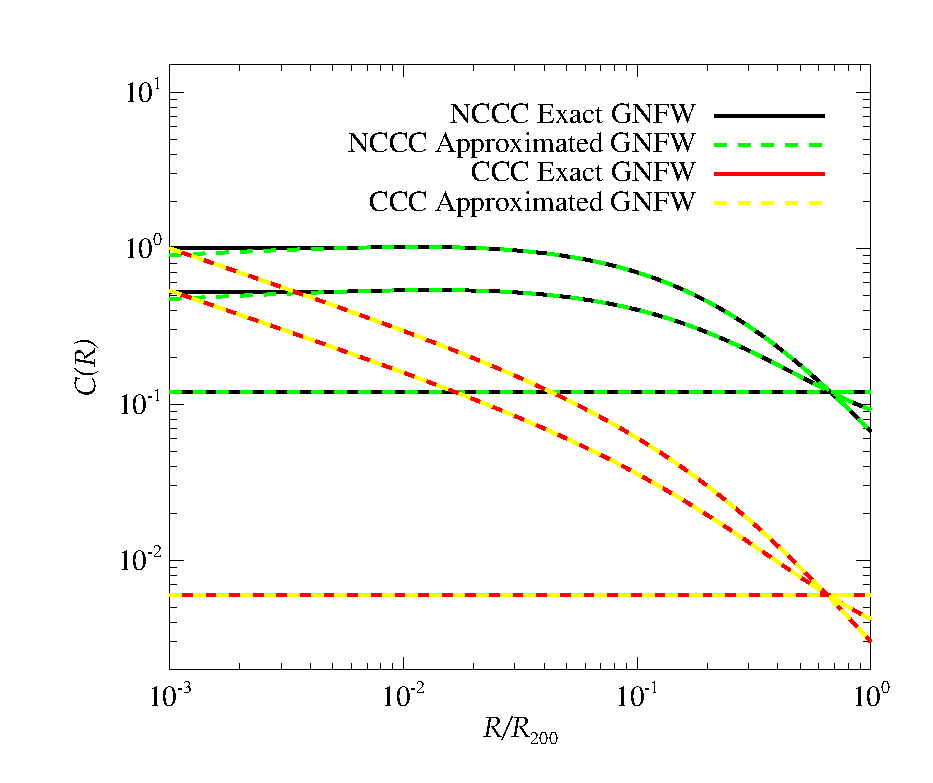
\includegraphics[width=0.5\textwidth]{figures/CR_profiles_REXexactVSfake.eps}
\caption{Comparison of the exact and approximate solutions for $C(R)$ in the
  case of our GNFW profile. In the latter case, we use the formulae by
  \protect\cite{2011A&A...527A..99E} but adopt $P(R)/P_{0}=n_{\rmn{e,GNFW}}(R)/n_{0}$
  for this comparison only, i.e., we assume here an isothermal ICM. We show the GNFW
  profiles for NCCCs and CCCs, as derived in Section~\ref{sec:2.2}. For each of
  these profile classes, we show three different cases of
  $\gamma_{\rmn{tu}}=100$, 10, and 1 (top to bottom). We normalize $C(R)$ for
  the advection dominated case ($\gamma_{\rmn{tu}}=100$) at $R=10^{-3}R_{200}$
  and and require CR number conservation during CR streaming. Note that the
  value for $C(10^{-3}R_{200},\gamma_{\rmn{tu}}=100)$ in the CCC case is
  identical for the exact solution and its approximation, while there is a small
  difference of about 9\% in the NCCC case. We adopt $\alpha=2.3$.}
\label{fig:REXexactVSfake}
\end{figure}

We want to extend this result to account for (i) our GNFW gas profiles of
Section~\ref{sec:2.2}, (ii) the universal temperature drop in the cluster
outskirts, and (iii) merge it with the universal cluster mass-scaling of the CR
normalization, $\tilde{C}$, obtained from hydrodynamical simulations
\citep{2010MNRAS.409..449P}.  Therefore, we adopt the extended profile,
$C_{\rm{extended}} = \tilde{C}(R) (\rho_{\rmn{gas}}(R)/m_\rmn{p}) (T(R)/T_0)$, of
equation~(\ref{eq:Cf}). We note that for such a choice, there does not any more
exist an analytical solution to equation~(\ref{eg:rhoCR_1}) as in
\cite{2011A&A...527A..99E}. This results in a 5-order equation and a numerical
solution would not be of practical use for every cluster in our large MultiDark
sample. For simplicity, we adopt the formulae above also for our extended
model. I.e., we adopt
$C(R)=C_{0}(\rho_{\rmn{CR}}(R)/\rho_{\rmn{CR},0})^{\beta_{\rmn{CR}}}$ within
$R_{\pm}$ of equation~(\ref{eq:Rpm}), with $\rho_{\rmn{CR}}$ defined by
equation~(\ref{eg:rhoCR_1}) where $C_{\rmn{extended}}$ enters through the
advective CR profile, $\eta(R)$, of equation~(\ref{eq:eta}), and $C(R) =
C(R_{\pm})$ for $R > R_{+}$ and $R < R_{-}$, respectively.  Note that, in our
formalism, $R_{\rmn{c}}$ of equation~(\ref{eq:Rpm}) becomes the characteristic
radius of our GNFW gas profile of Section~\ref{sec:2.2}, i.e., $R_{\rmn{c}} =
0.2 R_{500}$, and $\beta_{\rmn{cl}}=0.8$ (we checked that varying the value of
$\beta_{\rmn{cl}}$ between 0.4 and 1.2 has no impact).  The relevant factors are
$\gamma_{\rmn{tu}}$ and the exponential factor of
equation~(\ref{eg:rhoCR_1}). As we will see in the following, the two radii
$R_{\pm}$ are not critically affected by the form of $\eta(R)$. Therefore,
despite the approximation, this approach captures the main CR transport effects.

Assuming our GNFW gas profile instead of a standard $\beta$-profile for the
electron density, so adopting $P(R)/P_{0}=n_{\rmn{e,GNFW}}(R)/n_{0}$, there
exist an exact analytical solution to equation~(\ref{eg:rhoCR_1}) as in
\cite{2011A&A...527A..99E}. In order to evaluate the systematic error that we
are introducing with the approach described above, in
Fig.~\ref{fig:REXexactVSfake}, we compare the \emph{exact} solution for $C(R)$
in the case of our GNFW profile with the \emph{approximate} solution where we
use the formulae by \cite{2011A&A...527A..99E}, and only substitute the electron
$\beta$-profile for our GNFW profiles (with $R_{\rmn{c}} = 0.2 R_{500}$,
$\beta_{\rmn{cl}}=0.8$). In this last case, we fix $R_{-}=10^{-3}R/R_{200}$ to
mimic the typical $R_{-}$ value of the exact solution, otherwise an unphysical
step feature would appear at $\leq10^{-2}R/R_{200}$. This latter approximation
is kept in our extended model, which however has no impact on the model surface
brightness and total luminosity. There is almost no difference between the two
cases, as shown by Fig.~\ref{fig:REXexactVSfake}. This shows that the approach
presented here to construct our extended model can be safely followed in order to
derive a fully working parametrization which captures the main CR transport
effects.

%\begin{figure*}[t!]
%\centering
%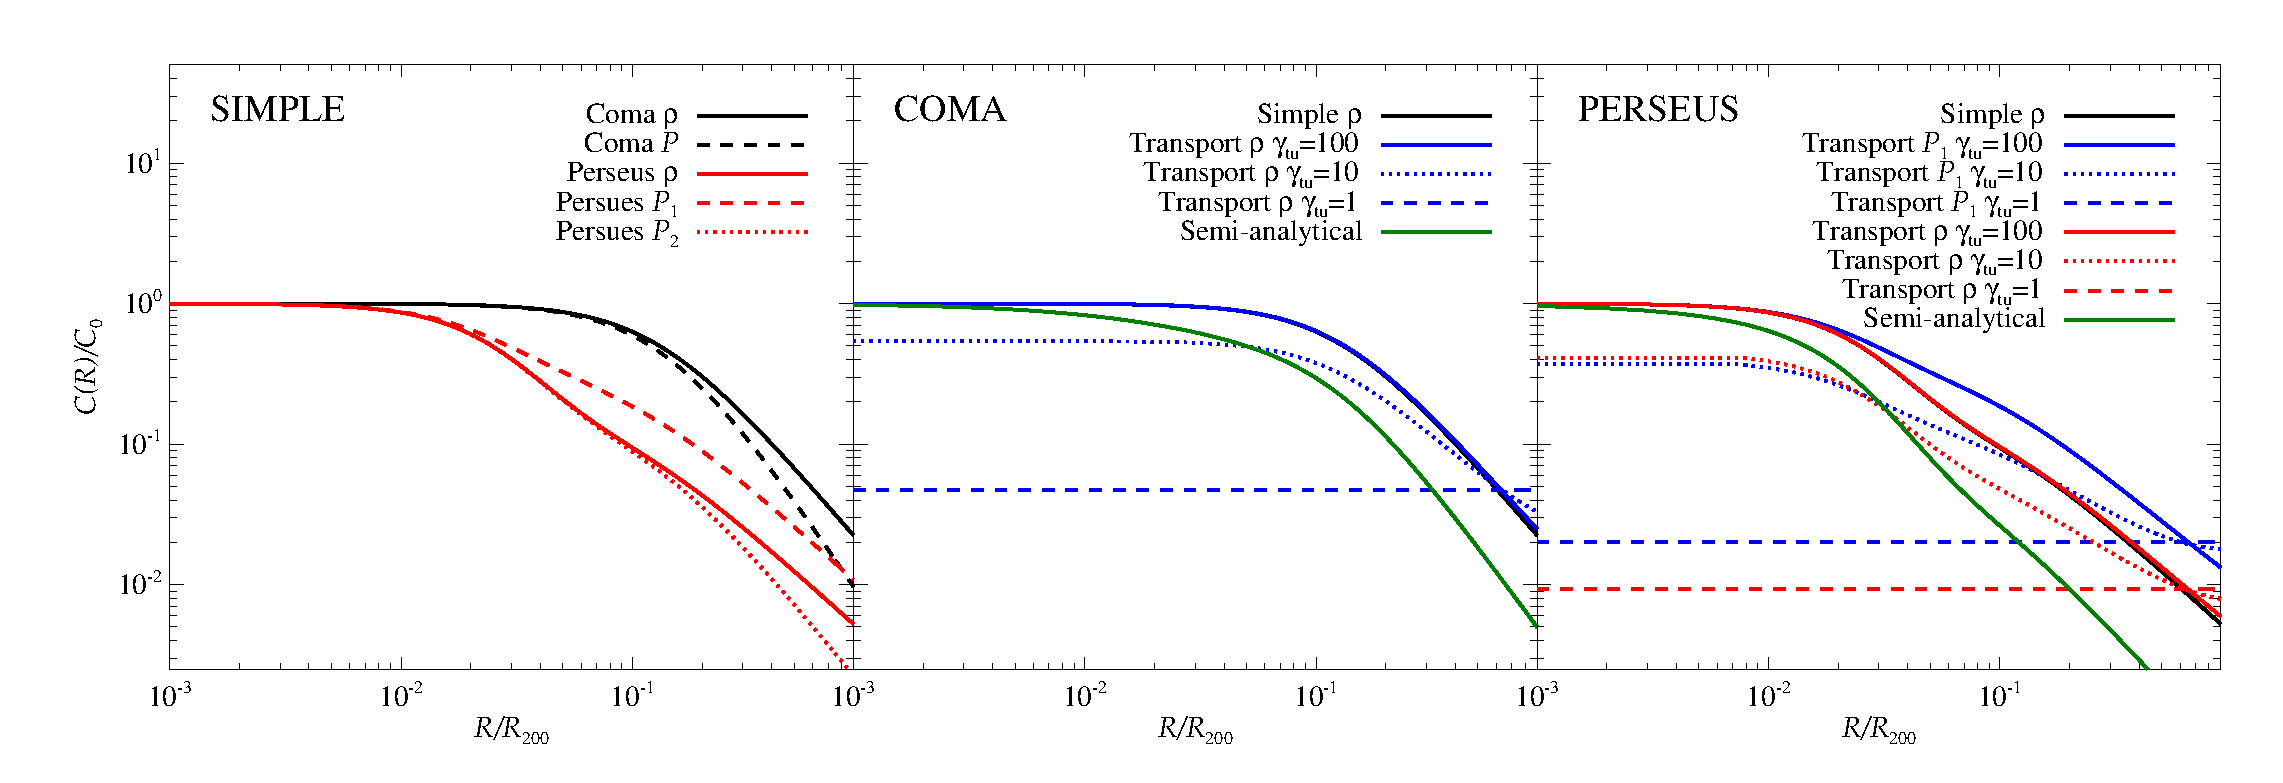
\includegraphics[width=0.99\textwidth]{figures/CR_profiles_simple_comparison.eps}
%\caption{Comparison of different CR profiles. The left plot shows the \emph{simple} advective $C_{\rmn{adv}}$ of equation~(\ref{eq:Csimple_1}) for the Coma and Perseus cases both neglecting the temperature dependence ($\rho$) and considering it ($P$). The temperature profile of Coma has been modified so that it follows the characteristic decline toward the cluster periphery. Perseus is a CCC and it is characterized by a central dip in the temperature profile which may importantly affect the final CR profile, so we adopt the temperature profile as given in \cite{2003ApJ...590..225C} ($P_{1}$). We also show the case where we only apply the characteristic decline toward the cluster periphery ($P_{2}$). The other two right plots show the \emph{transport} case of equation~(\ref{eq:Ctransport}) for Coma and Perseus for different values of $\gamma_{\rmn{tu}}$ in comparison with the \emph{simple} case. Additionally shown is the result in case of $C(R)=C_{\rmn{semi-analytical}}(R)=\tilde{C}(R)\rho_{\rmn{gas}}(R)/m_{\rmn{p}}$ where $\tilde{C}(R)$ is the mass-dependent universal normalization CR profile found in cosmological simulations \citep{2010MNRAS.409..449P}. The \emph{simple} and \emph{semi-analytical} profiles are normalized at $C_{0}=C(0)$. In the transport case, we fix the CR number for $\gamma_{\rmn{tu}}=100$ using equation~(36) of \cite{2011A&A...527A..99E}, while integrating the cluster volume within $R_{200}$, and require CR number conservation during CR streaming. We adopt $\alpha=2.3$.}
%\label{fig:simpleVStransport}
%\end{figure*}
%
%
%In Fig.~\ref{fig:simpleVStransport}, we show a comparison between $C_{\rmn{adv}}$ of 
%equation~(\ref{eq:Csimple_1}) and $C$ of equation~(\ref{eq:Ctransport}) considering the 
%NCCC Coma and CCC Perseus cases. While for Coma we adopt the $\beta$-profile of 
%\citet{1992A&A...259L..31B}, Perseus needs a double-$\beta$ profile. We adopt both the 
%approximation $P(R)/P_{0}=n_{\rmn{e}}(R)/n_{0}$ and the proper Perseus pressure profile 
%(X-ray data from \citealp{2003ApJ...590..225C}). Note that the \cite{2011A&A...527A..99E} 
%formalism is exact only for the approximation $P(R)/P_{0}=n_{\rmn{e}}(R)/n_{0}$ where $n_{\rmn{e}}$ 
%is a $\beta$-profile. Nevertheless, we adopt the above formulae also for Perseus as a good approximation, 
%i.e., we adopt $C(R)=C_{0}(\rho_{\rmn{CR}}(R)/\rho_{\rmn{CR},0})^{\beta_{\rmn{CR}}}$
%within $R_{\pm}$ of equation~(\ref{eq:Rpm}), and $C(R) = C(R_{\pm})$ for $R > R_{+}$ 
%and $R < R_{-}$, respectively; we take $R_{\rmn{c}}$ in equation~(\ref{eq:Rpm}) to be equal to the Perseus 
%double-$\beta$ profile outer core radius and fix $\beta_{\rmn{cl}}=0.8$. The relevant 
%parameters are $\gamma_{\rmn{tu}}$ and the exponential factor of equation~(\ref{eg:rhoCR_1}). 
%In fact, as we will see in the following, the two radii $R_{\pm}$ are not critically affected 
%by the detail of $\eta(R)$. Therefore, despite the approximation, this approach captures the 
%main CR transport effects also for the Perseus case. 
%
%In Fig.~\ref{fig:simpleVStransport}, we additionally show the result in case 
%$C(R)=C_{\rmn{semi-analytical}}(R)=\tilde{C}(R)\rho_{\rmn{\rmn{gas}}}(R)/m_{\rmn{p}}$ 
%where $\tilde{C}(R)$ is the universal normalization CR profile found in cosmological 
%simulations \citep{2010MNRAS.409..449P}. As expected, the CR profile driven by 
%simulations is characterized by a more centrally peaked profile with respect to the 
%analytical case. Note also the flatter profile of Coma with respect to Perseus, which 
%reflects their NCCC and CCC classification, respectively. Finally, the effect of varying 
%the turbulent cluster state by means of $\gamma_{\rmn{tu}}$ can be clearly appreciated.


%%%%%%%%%%%%%%%%%%%%%%%%%%%%%%%%%%%%%%%%%%%%%%%%%%%%%%%%%%%%%%%%%%%
%%%%%%%%%%%%%%%%%%%%%%%%%%%%%%%%%%%%%%%%%%%%%%%%%%%%%%%%%%%%%%%%%%%

\section{Radio Emission}
\label{app:A}

The factor $A_{\nu}$ in the equation for the radio synchrotron emissivity,
equation~(\ref{eq:jnu}), is given by (see also \citealp{2008MNRAS.385.1211P} and
\citealp{2011A&A...527A..99E})
%
\begin{equation}
A_{\nu} = A_{\rmn{E_{synch}}} \frac{16^{2-\alpha_{\rmn{e}}}\sigma_{\rmn{pp}}m_{\rmn{e}}c^{2}}{(\alpha_{\rmn{e}}-2)\sigma_{\rmn{T}}\epsilon_{B_{\rmn{C}}}m_{\rmn{p}}}\left(\frac{m_{\rmn{p}}
}{m_{\rmn{e}}}\right)^{\alpha_{\rmn{e}}-2} \left(\frac{m_{\rmn{e}}c^{2}}{\rmn{GeV}}\right)^{\alpha_{\rmn{e}}-1} \, ,
\end{equation}
%
with
%
\begin{equation}
A_{\rmn{E_{synch}}} = \frac{\sqrt{3\pi}}{32\pi}\frac{B_{\rmn{c}}e^{3}}{m_{\rmn{e}}c^{2}}\frac{\alpha_{\rmn{e}}+\frac{7}{3}}{\alpha_{\rmn{e}}+1}\frac{\Gamma\left(\frac{3\alpha_{\rmn{e}}-1}{12}\right)\Gamma\left(\frac{3\alpha_{\rmn{e}}+7}{12}\right)\Gamma\left(\frac{\alpha_{\rmn{e}}+5}{4}\right)}{\Gamma\left(\frac{\alpha_{\rmn{e}}+7}{4}\right)} \, ,
\end{equation}
%
where $\alpha_{\rmn{e}}=\alpha+1$, the effective inelastic cross-section for
proton-proton interactions is $\sigma_{\rmn{pp}} =
32~(0.96+\rmn{e}^{4.42-2.4\alpha})$, $B_{\rmn{c}} = \sqrt{ 8 \pi
  \epsilon_{B_{\rmn{c}}}} \simeq 31 \left( \nu/\rmn{GHz} \right)~\mu$G, and
$\Gamma$ is the Gamma-function
\citep{1965hmfw.book.....A}. $A_{\rmn{E_{synch}}}$ is given in units of erg, and
$A_{\nu}$ is given in units of erg~cm$^{3}$~g$^{-1}$~sr$^{-1}$.

The generalization of the radio emissivity, $j_{\nu}$, to account for three CR populations,
each characterized by different power-law spectra and the inclusion of the
normalization parameter $g_{\rmn{CR}}$, following \cite{2010MNRAS.409..449P}, is
straight forward. We obtain
%
\begin{eqnarray}
j_{\nu,\rmn{extended}} & = &g_{\rmn{CR}} C(R) \rho_{\rmn{gas}}(R) \frac{\epsilon_{\rmn{B}}(R)}{\epsilon_{\rmn{B}}(R)+\epsilon_{\rmn{CMB}}} \nonumber \\
& \times & \Sigma_{i=1}^{3} \Delta_{i} A_{\nu,i} \left( \frac{\epsilon_{\rmn{B}}(R)}{\epsilon_{B_{\rmn{c}}}} \right)^{\frac{\alpha_{i}-2}{4}}  \, ,
\end{eqnarray}
%
where the sum is over the three CR spectral indexes $\alpha_{i}=(2.55,2.3,2.15)$
with the corresponding factors $\Delta_{i} = (0.767, 0.143, 0.0975)$ found by
\cite{2010MNRAS.409..449P}.
 

%%%%%%%%%%%%%%%%%%%%%%%%%%%%%%%%%%%%%%%%%%%%%%%%%%%%%%%%%%%%%%%%%%%
%%%%%%%%%%%%%%%%%%%%%%%%%%%%%%%%%%%%%%%%%%%%%%%%%%%%%%%%%%%%%%%%%%%

\section{Gamma-ray Emission}
\label{app:C}

The gamma-ray flux above an energy $E_{\gamma}$ is given by (e.g.,
\citealp{2010MNRAS.409..449P})
%
\begin{equation}
F_{\gamma} (>E_{\gamma}) = \frac{1}{4\pi D^{2}} \int dV  \lambda_{\gamma}(R)\, ,
\end{equation}
%
where the omnidirectional (i.e., integrated over the $4\pi$ solid angle)
gamma-ray emissivity above $E_{\gamma}$ is $ \lambda_{\gamma}(R)=A_{\gamma} C(R)
\rho_{\rmn{gas}}(R)$. The parameter $A_{\gamma}$ is \citep{2010MNRAS.409..449P}
%
\begin{eqnarray}
A_{\gamma} = g_{\rmn{CR}} D_{\gamma,\rmn{break}} \frac{4 m_{\pi^{0}} c}{3 m_{\rmn{p}}^{2}} \Sigma_{i=1}^{3} \Delta_{i} \frac{\sigma_{\rmn{pp},i}}{\alpha_{i} \delta_{i}} \left( \frac{m_{\rmn{p}}}{2 m_{\pi^{0}}} \right)^{\alpha_{i}} \times \nonumber \\
\times \left[ \beta_{x} \left( \frac{\alpha_{i}+1}{2\delta_{i}}, \frac{\alpha_{i}-1}{2\delta_{i}} \right) \right]_{x_{1}}^{x_{2}} \, ,
\end{eqnarray}
%
where $x_{j}=\{ 1 + [ m_{\pi^{0}}c^2/(2E_{\gamma,j})]^{2\sigma_{i}} \}$, $\left[ \beta_{x}(a,b) \right]_{x_1}^{x_2} =
\beta_{x_2}(a,b)-\beta_{x_1}(a,b)$ where $\beta$ denotes the incomplete
Beta-function \citep{1965hmfw.book.....A}, and
$\delta_{i}=0.14\alpha_{i}^{-1.6}+0.44$. The term $D_{\gamma,
  \rmn{break}}=D_{\gamma}(E_{\gamma},E_{\gamma,\rmn{break}})$ represents
diffusive CR losses due to escaping protons from the cluster at the equivalent
photon energy for the break $E_{\gamma, \rmn{break}}$ (see
\citealp{2010MNRAS.409..449P} for details). $A_{\gamma}$ is given in units of
cm$^3$~s$^{-1}$~g$^{-1}$.



%%%%%%%%%%%%%%%%%%%%%%%%%%%%%%%%%%%%%%%%%%%%%%%%%%%%%%%%%%%%%%%%%%%
%%%%%%%%%%%%%%%%%%%%%%%%%%%%%%%%%%%%%%%%%%%%%%%%%%%%%%%%%%%%%%%%%%%

\section{Observational Radio-to-X-ray Scaling relation and Luminosity Function}
\label{app:D}

For comparison with the observed 1.4~GHz radio-to-X-ray scaling relation, we
include almost all RHs of the sample by \cite{2011A&A...527A..99E}. 
We exclude RXCJ1314.4-2515 and Z7160 because they lack bolometric X-ray measurements. 
%and A2626 because its X-ray luminosity is very low placing it as an extreme outlier. 
We add to our sample the clusters Ophiuchus, A2029 and A1835
\citep{2009A&A...499..371G}. The bolometric X-ray luminosities,
$L_{\rmn{X,bol}}$, of clusters hosting giant radio halos are taken from
\cite{2009A&A...507..661B}, while $L_{\rmn{X,bol}}$ values of cluster hosting
for mini-halos are taken from \cite{2002ApJ...567..716R},
\cite{Boehringer:1998vv} and ACCEPT. In the cases where measurement
uncertainties for X-ray and radio luminosities are not reported, we adopt a
$10\%$ uncertainty. Our final RH sample has a median redshift of
$z\approx0.18$. In the left panel of Fig.~\ref{fig:PLSZ}, we show the
corresponding radio-to-X-ray scaling relation which is well fit by $\log_{10}
(L_{1.4~\rmn{GHz}}/h_{70}^{-2}~\rmn{erg}~\rmn{s}^{-1}~\rmn{Hz}^{-1}) = A +
B~\log_{10} (L_{\rmn{X,bol}}/h_{70}^{-2}~\rmn{erg}~\rmn{s}^{-1})$, with
$A=-37.204\pm1.838$, $B=1.512\pm0.041$, and scatter $\sigma_{yx} \approx
0.52$. Regarding the clusters with upper limits on the diffuse radio emission in
the sample of \cite{2011A&A...527A..99E}, we select only those 8 clusters with
ACCEPT measurements to obtain a homogeneous data set in $L_{\rmn{X,bol}}$ (note
that there are a number of clusters with upper limits on $L_{1.4~\rmn{GHz}}$ for
which there are only soft-band X-ray luminosities available).

In Fig.~\ref{fig:RLFobs}, we make an attempt to construct an RLF from existing
X-ray flux-limited radio surveys. There exist two such studies: the
\cite{1999NewA....4..141G} survey with NVSS at $1.4$~GHz and the
\cite{VenturiGMRT_1,VenturiGMRT_2} survey with GMRT at $610$~MHz by. We only
select RHs, i.e., we do not consider radio relics or other diffuse radio
emissions of unclear classification. The 1.4~GHz NVSS survey contains 13~RHs out
of 205 analyzed clusters while the 610~MHz GMRT survey contains 6 RHs out of the
34 observed. The sample finally analyzed by \cite{VenturiGMRT_1,VenturiGMRT_2}
is composed by 50 clusters and we can also build a corresponding RLF at 1.4~GHz
using the 12 present RHs. The fraction of radio-loud clusters is about 6\%, 18\%
and 24\% for the NVSS 1.4~GHz, GMRT 610~MHz and GMRT 1.4~GHz sample,
respectively. The corresponding median redshift is 0.18, 0.26 and 0.25. We
calculate the RLF using the classical $V_{\rmn{max}}$ estimator (e.g.,
\citealp{1976ApJ...207..700F}) correcting for the sample incompleteness and
survey sky coverage. The most problematic aspect in obtaining these RLFs, apart
from the few available objects, is the calculation of a meaningful flux
limit. We obtain such a limit by fitting the upper envelope of the
luminosity-distance distribution of a given sample, as shown in the insets of
Fig.~\ref{fig:RLFobs}, following the procedure adopted by
\cite{2011arXiv1106.5494B}. Note that it is particularly ambiguous to calculate
a meaningful flux limit for the GMRT survey due to its poor luminosity-distance
distribution. We decide therefore to take the 1.4~GHz NVSS RLF as reference in
our comparisons with observation. However, we want to stress that several issues
can affect this result, such as the small sample size that impacts the resulting
flux limit, and the Malmquist and Eddington biases. Indeed, the very different
fraction of radio loud clusters obtained from different samples is one clear
indicator of the large uncertainty in the RLF.

\begin{figure} 
\centering
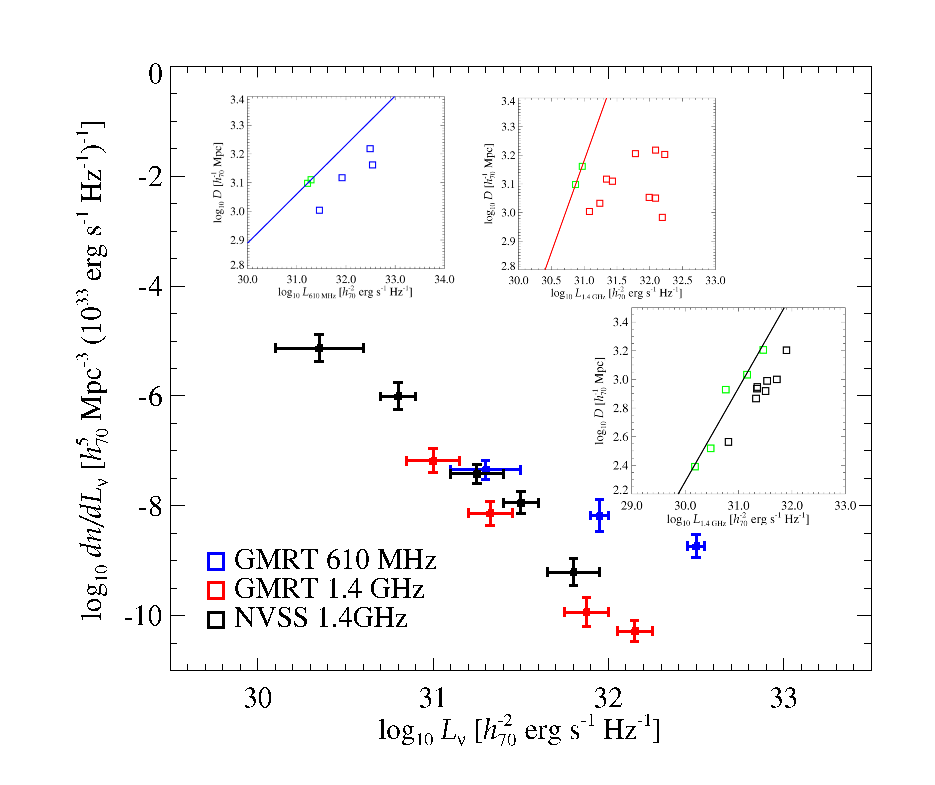
\includegraphics[width=0.48\textwidth]{figures/RLF_observations.eps}
\caption{RH luminosity function obtained from existent observations. The insets
  show the sample luminosity-distance distributions (see main text for details)
  where the solid line is the fit to the upper envelope population (indicated in
  green) employed to calculate the flux limit for the classical $V_{\rmn{max}}$
  estimator. The choice of the upper envelope population is somehow arbitrary,
  particularly in the GMRT cases due to the poor luminosity--distance
  distributions. The horizontal error bars represent the mass bins while the
  vertical error bars are Poissonian uncertainties.}
\label{fig:RLFobs}
\end{figure}

%Finally, in Fig.~\ref{fig:RLF1.4_fluxNVSS}, we compare the cumulative number of RHs above a certain flux limit at 1.4~GHz obtained by our model realization described in Section~\ref{sec:4}, adopting a fraction of 10\% of radio-loud clusters, with the NVSS survey result (data is taken from \citealp{2010A&A...509A..68C}). We repeat the steps done in Section~5.2 in order to obtain an analytical model describing the number of RHs expected in our model per unit luminosity and per unit comoving volume. We then use equationx~(\ref{eq:NtotRH}) to calculate the cumulative number of RHs above a given flux. The luminosity integration is limited to $\log_{10} L_{1.4~\rmn{120MHz}} \geq 28$ to exclude the turn-over at low luminosities caused by incompleteness, while the redshift integration is limited to the range covered by the NVSS survey of $0.044 \leq z \leq 0.2$ \citep{1999NewA....4..141G}. We find a agreement comparison between our model and the observational result of the NVSS survey.

%\begin{figure} 
%\centering
%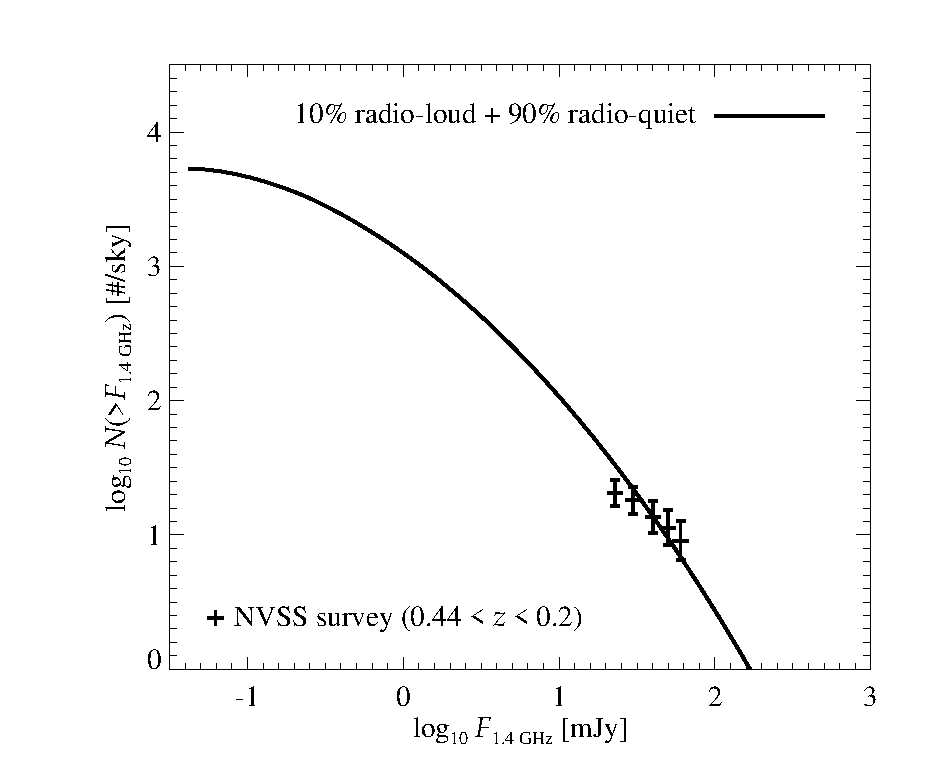
\includegraphics[width=0.48\textwidth]{figures/RLF_1.4_flux_NVSS.eps}
%\caption{Cumulative number of RHs above a certain flux limit in an all-sky
%  survey at 1.4~GHz for $0.044 \leq z \leq 0.2$. The black line shows the result 
%  obtained with the model realization described in Section~\ref{sec:4}, adopting 
%  a fraction of 10\% of radio-loud clusters, integrating within the redshift range covered 
%  by the NVSS survey (black data points).}
%\label{fig:RLF1.4_fluxNVSS}
%\end{figure}

\end{appendix}


%%%%%%%%%%%%%%%%%%%%%%%%%%%%%%%%%%%%%%%%%%%%%%%%%%%%%%%%%%%%%%%%%%
%%%%%%%%%%%%%%%%%%%%%%%%%%%%%%%%%%%%%%%%%%%%%%%%%%%%%%%%%%%%%%%%%%
\label{lastpage}

\end{document}

%\del{In comparing with observations, we take as reference
%  \cite{2010MNRAS.406.1773M}. There are however many other works on this scaling
%  relation, in particularly we recall the HIghest X-ray FLUx Galaxy Cluster
%  Sample (HIFLUGCS; \citealp{2002ApJ...567..716R}), the REXCESS
%  \citep{2009A&A...498..361P} sample, and the 115 \emph{Chandra} cluster sample
%  of \cite{2007ApJ...668..772M}. The results on the slopes of the $L-M$ relation
%  can vary significantly between different samples. While the slope of
%  \cite{2010MNRAS.406.1773M} is $1.63\pm0.06$,
%  \cite{2002ApJ...567..716R}\footnote[8]{Note that we are quoting the
%    $L_{\rmn{bol}}-M_{200}$ results of \cite{2002ApJ...567..716R}.} found values
%  between $1.72\pm0.09$ and $1.89\pm0.08$ (depending on the fit procedure, which
%  also can affect the final result), \cite{2009A&A...498..361P} found
%  $2.08\pm0.13$ and \cite{2007ApJ...668..772M} found
%  $1.96\pm0.10$. Discrepancies can come from many different sources but likely
%  are to be charged to the selection criteria of the different samples as
%  recently pointed out also by \cite{2011arXiv1109.3708R}. Samples which differ
%  in, e.g., redshift distribution, mass range, fitting procedure and biases
%  treatment, and, of course, the used instrument, can give and actually gave
%  different results. Therefore we decided to take as reference the
%  \cite{2010MNRAS.406.1773M} work because it is very recent, their sample is
%  composed by a high number (238) of objects, and, more importantly, their
%  analysis takes self-consistently into account all selection effects,
%  covariances, systematic uncertainties and the cluster mass function (see also
%  \citealp{2010MNRAS.406.1759M}).}
